\documentclass[aspectratio=169]{beamer}
\newcommand{\outlinecols}{1}
\newcommand{\monthyeardate}{\ifcase \month \or Jan.\or Feb.\or Mar.\or Apr.\or May \or Jun.\or Jul.\or Aug.\or Sept.\or Oct.\or Nov.\or Dec.\fi~\number\year}
\newcommand{\insertframetitle}{}
\date{\monthyeardate}

\setbeamertemplate{caption}[numbered]
\setbeamertemplate{frametitle continuation}{}
\setbeamertemplate{bibliography item}[text]
\mode<presentation> {
  \usetheme{Madrid}
  \usefonttheme{professionalfonts}
  \setbeamertemplate{headline}{}
  
  \renewcommand*\footnoterule{%
    \usebeamercolor[fg]{block title}%
    \usebeamerfont{block title}%    
    Refereces%
    \vskip.5\baselineskip%
  }
  
  \setbeamertemplate{footnote}
  {
    \parindent 1em\noindent%
    \raggedright
    \hbox to 0.4em{\hfil\insertfootnotemark}\insertfootnotetext\par%
  }
  \setbeamertemplate{footline}{
    % author: Ang, Li (ang.li.1997@icloud.com)
    \leavevmode%
    \hbox{%
      \begin{beamercolorbox}[wd=.18\paperwidth,ht=2.25ex,dp=1ex,center]{author in head/foot}%
        \usebeamerfont{author in head/foot}\insertshortauthor
      \end{beamercolorbox}%
      \begin{beamercolorbox}[wd=.64\paperwidth,ht=2.25ex,dp=1ex,center]{title in head/foot}%
        \usebeamerfont{title in head/foot}\insertshorttitle
        \ifdefempty{\insertsectionhead}{}{
          \hspace*{1em}$\blacktriangleright$\hspace*{1em}
          \usebeamerfont{section in head/foot}\insertsectionhead
        }
        \ifdefempty{\insertsubsectionhead}{}{
          \hspace*{1em}$\blacktriangleright$\hspace*{1em}
          \usebeamerfont{subsection in head/foot}\insertsubsectionhead
        }
        % \ifdefempty{\insertframetitle}{}{
        %   \hspace*{1em}$\blacktriangleright$\hspace*{1em}
        %   \usebeamerfont{section in head/foot}\insertframetitle
        % }
      \end{beamercolorbox}%
      \begin{beamercolorbox}[wd=0.18\paperwidth,ht=2.25ex,dp=1ex,right]{author in head/foot}%
        \usebeamerfont{date in head/foot}\insertshortdate \hspace*{2em}
        \insertframenumber{} / \inserttotalframenumber \hspace*{1em}
      \end{beamercolorbox}}%
    \vskip0pt%
  }
  \beamertemplatenavigationsymbolsempty
}

\RequirePackage{graphicx} % Allows including images
\RequirePackage{booktabs} % Allows the use of \toprule, \midrule and \bottomrule in tables
\RequirePackage{multirow}
\RequirePackage{color}
\RequirePackage{bm}
\RequirePackage{amsthm}
\RequirePackage{amsmath}
\RequirePackage{amssymb}
\RequirePackage{mathabx}
\RequirePackage{epstopdf}
\RequirePackage{animate}
\RequirePackage{multirow}
\RequirePackage{enumerate}
\RequirePackage{multicol}

\RequirePackage[style=authoryear,sorting=none]{biblatex}
\setbeamertemplate{bibliography item}{~~$\blacktriangleright $}
\definecolor{brightmaroon}{rgb}{0.76, 0.13, 0.28}
\definecolor{myblue}{rgb}{0.15, 0.29, 0.93}
\newcommand{\citep}[1]{{\color{myblue}(\cite{#1})}}
\renewcommand*{\nameyeardelim}{\addcomma\space}

\setbeamerfont{author}{size=\Large}
\setbeamerfont{institute}{size=\small}
\setbeamerfont{footnote}{size=\tiny}
\RequirePackage{siunitx}
\RequirePackage{xcolor}
\RequirePackage{listings}
\RequirePackage{algorithm}
\RequirePackage{algpseudocode}
\RequirePackage{subfigure}
\RequirePackage{cleveref}
\RequirePackage{tcolorbox}
\RequirePackage{tikz}
\RequirePackage{ctex}

\setbeamercovered{highly dynamic}

\makeatletter
% save the meaning of \@footnotetext
\let\BEAMER@footnotetext\@footnotetext
\makeatother

\RequirePackage{setspace}

\makeatletter
% restore the meaning of \@footnotetext
\let\@footnotetext\BEAMER@footnotetext
% patch the relevant command to do single spacing in footnotes
\expandafter\patchcmd\csname beamerx@\string\beamer@framefootnotetext\endcsname
{\reset@font}
{\def\baselinestretch{\setspace@singlespace}\reset@font}
{}{}
\makeatother

\newenvironment<>{varblock}[2][.9\textwidth]{%
  \setlength{\textwidth}{#1}
  \begin{actionenv}#3%
    \def\insertblocktitle{#2}%
    \par%
    \usebeamertemplate{block begin}}
    {\par%
    \usebeamertemplate{block end}%
  \end{actionenv}}

\setbeamertemplate{theorems}[numbered]

\renewcommand{\Call}{\textbf{Call~}}
\algnewcommand{\IIf}[1]{\State\algorithmicif\ #1\ \algorithmicthen}
\algnewcommand{\ElseII}{\algorithmicelse\ }
\algnewcommand{\EndIIf}{\unskip\ \algorithmicend\ \algorithmicif}
\newcommand{\hl}[1]{{\bfseries\color{myblue}{#1}}}
\newcommand{\HL}[1]{{\color{myblue}{#1}}}
\newcommand{\redhl}[1]{{\bfseries\color{brightmaroon}{#1}}}
\newcommand{\redHL}[1]{{\color{brightmaroon}{#1}}}
\lstset{
  language=C++,
  numbers=left,
  keywordstyle= \color{blue!70},
  commentstyle= \color{red!50!green!50!blue!50},
  frame=tb,
  rulesepcolor= \color{red!20!green!20!blue!20} ,
  xleftmargin=2em, aboveskip=1em,
  framexleftmargin=2em
}

\ifundef{\outlinecols}{\newcommand{\outlinecols}{1}}{}
\ifnum \outlinecols > 1
  \newcommand{\liangoutline}{
    \begin{multicols}{\outlinecols}
      \tableofcontents[hidesubsections,pausesections]
    \end{multicols}
  }
  \newcommand{\liangoutlinesection}{
    \begin{multicols}{\outlinecols}
      \tableofcontents[currentsection,hideothersubsections]
    \end{multicols}
  }
  \newcommand{\liangoutlinesubsection}{
    \begin{multicols}{\outlinecols}
      \tableofcontents[currentsection,subsectionstyle=show/shaded/hide]
    \end{multicols}
  }
\else
  \newcommand{\liangoutline}{
    \tableofcontents[hidesubsections,pausesections]
  }
  \newcommand{\liangoutlinesection}{
    \tableofcontents[currentsection,hideothersubsections]
  }
  \newcommand{\liangoutlinesubsection}{
    \tableofcontents[currentsection,subsectionstyle=show/shaded/hide]
  }
  
\fi

\newcommand{\outlineframe}{
  \begin{frame}
    \liangoutline
  \end{frame}
}

\AtBeginSection[]
{
  \begin{frame}
    \liangoutlinesection
  \end{frame}
}
\AtBeginSubsection[]
{
  \begin{frame}
    \liangoutlinesubsection
  \end{frame}
}
\newcommand{\ThankFrame}{
  \section*{请老师和同学们批评指正!}
  \begin{frame}
    \kai\fontsize{60pt}{60pt}\selectfont
    {\centerline{请老师和同学们}}
    {\centerline{批评指正!}}
  \end{frame}
}
\newcommand{\RefFrame}{
  \section*{Referencs}
  \begin{frame}[allowframebreaks]{Referencs}
    \printbibliography
  \end{frame}
}

\newenvironment{tabenumerate}[1]{
  \begin{columns}
    \begin{column}{#1}\end{column}
    \begin{column}{\textwidth-#1}
      \begin{enumerate}[<+->]
        }{
      \end{enumerate}
    \end{column}
  \end{columns}
}


\def\Xint#1{\mathchoice
  {\XXint\displaystyle\textstyle{#1}}%	
  {\XXint\textstyle\scriptstyle{#1}}%	
  {\XXint\scriptstyle\scriptscriptstyle{#1}}%	
  {\XXint\scriptscriptstyle\scriptscriptstyle{#1}}%	
  \!\int}

\def\XXint#1#2#3{{\setbox0=\hbox{$#1{#2#3}{\int}$}
      \vcenter{\hbox{$#2#3$}}\kern-.5\wd0}}
\def\ddashint{\Xint=}
\def\dashint{\Xint-}

\newcommand{\colorBOX}[5][myblue!10]{%
  \vspace{-2mm}%
  \begin{center}%
    \begin{tcolorbox}[colback=#1, width=#2, colframe=white, arc=1mm, auto outer arc, boxrule=0pt]%
      \vspace{#3}%-5mm
      #5%
      \vspace{#4}%-7mm
    \end{tcolorbox}%
  \end{center}%
}

\newcommand{\FigAndTex}[3][.5\textwidth]{
  \begin{columns}
    \begin{column}{#1}
      \begin{center}
        #2
      \end{center}
    \end{column}
    \begin{column}{\textwidth-#1}
      #3
    \end{column}
  \end{columns}
}

\newcommand{\TextAndFig}[3][.5\textwidth]{
  \begin{columns}
    \begin{column}{#1}
      #2
    \end{column}
    \begin{column}{\textwidth-#1}
      \begin{center}
        #3
      \end{center}
    \end{column}
  \end{columns}
}

\usepackage{xpatch}
\xpatchcmd{\itemize}{\def\makelabel}{%
  \setlength{\itemsep}{2ex}%
  \setlength{\parsep}{1ex}%
  \def\makelabel%
}{}{}

\setsansfont{Times New Roman}
\newCJKfontfamily\song{SimSun}[AutoFakeBold={4}]
\newCJKfontfamily\kai{KaiTi}[AutoFakeBold={4}]
\newCJKfontfamily\hei{SimHei}[AutoFakeBold={4}]
\newCJKfontfamily\xingkai{Xingkai SC Light}[AutoFakeBold={4}]

\setbeamerfont{normal text}{family=\kai,series=\mdseries} % ignored currently
\setbeamerfont{alerted text}{family=\kai,series=\mdseries}
\setbeamerfont{example text}{family=\kai,series=\mdseries}

\setbeamerfont{structure}{}
\setbeamerfont{tiny structure}{size=\tiny}

\setbeamerfont{title}{size=\Large,parent=structure,family=\hei,series=\bfseries}
\setbeamerfont{title in head/foot}{family=\pingfang,series=\mdseries}
\setbeamerfont{title in sidebar}{size=\tiny}

\setbeamerfont{subtitle}{size=\normalsize,parent=title,family=\hei,series=\bfseries}

\setbeamerfont{author}{size=\Large,family=\pingfang,series=\mdseries}
\setbeamerfont{author in head/foot}{family=\pingfang,series=\mdseries}
\setbeamerfont{author in sidebar}{size=\tiny}

\setbeamerfont{institute}{size=\normalsize,family=\kai,series=\mdseries}
\setbeamerfont{institute in head/foot}{family=\pingfang,series=\mdseries}
\setbeamerfont{institute in sidebar}{}

\setbeamerfont{date}{size=\normalsize,family=\kai,series=\mdseries}
\setbeamerfont{date in head/foot}{family=\pingfang,series=\mdseries}
\setbeamerfont{date in sidebar}{}

\setbeamerfont{page number in head/foot}{family=\pingfang,series=\mdseries}

\setbeamerfont{part name}{size=\LARGE}
\setbeamerfont{part title}{size=\LARGE,parent=title}

\setbeamerfont{section name}{size=\Large}
\setbeamerfont{section title}{size=\Large,parent=title}

\setbeamerfont{section in toc}{parent=structure}
\setbeamerfont{section in toc shaded}{parent=section in toc}
\setbeamerfont{section in head/foot}{family=\pingfang,series=\mdseries}
\setbeamerfont{section in sidebar}{size=\tiny}
\setbeamerfont{section number projected}{size=\small,parent={section in toc,projected text}}

\setbeamerfont{subsection name}{size=\large}
\setbeamerfont{subsection title}{size=\large,parent=title}

\setbeamerfont{subsection in toc}{}
\setbeamerfont{subsection in toc shaded}{parent=subsection in toc}
\setbeamerfont{subsection in head/foot}{family=\pingfang,series=\mdseries}
\setbeamerfont{subsection in sidebar}{}

\setbeamerfont{subsubsection in toc}{size=\footnotesize}
\setbeamerfont{subsubsection in toc shaded}{parent=subsubsection in toc}
\setbeamerfont{subsubsection in head/foot}{family=\pingfang,series=\mdseries}
\setbeamerfont{subsubsection in sidebar}{}

\setbeamerfont{headline}{parent={tiny structure}}
\setbeamerfont{footline}{parent={tiny structure}}

\setbeamerfont{sidebar}{size=\Tiny,parent={tiny structure}}
\setbeamerfont{sidebar left}{parent=sidebar}
\setbeamerfont{sidebar right}{parent=sidebar}

\setbeamerfont{frametitle}{parent=structure,size=\Large}
\setbeamerfont{framesubtitle}{parent=frametitle,size=\footnotesize}

\setbeamerfont{caption}{size=\small,family=\kai,series=\mdseries}
\setbeamerfont{caption name}{parent={structure,caption},family=\kai,series=\mdseries}

\setbeamerfont{button}{size=\tiny,family=\kai,series=\mdseries}

\setbeamerfont{block body}{family=\kai,series=\mdseries}
\setbeamerfont{block body alerted}{family=\kai,series=\mdseries}
\setbeamerfont{block body example}{family=\kai,series=\mdseries}
\setbeamerfont{block title}{size=\large,parent={structure,block body}}
\setbeamerfont{block title alerted}{parent={block title,alerted text}}
\setbeamerfont{block title example}{parent={block title,example text}}

\setbeamerfont{item}{family=\kai,series=\mdseries,parent=structure}
\setbeamerfont{subitem}{parent=item}
\setbeamerfont{subsubitem}{parent=subitem}

\setbeamerfont{item projected}{size=\tiny,parent={item,projected text}}
\setbeamerfont{subitem projected}{parent=item projected}
\setbeamerfont{subsubitem projected}{parent=subitem projected}

\setbeamerfont{itemize item}{parent=item}
\setbeamerfont{itemize subitem}{parent=subitem}
\setbeamerfont{itemize subsubitem}{parent=subsubitem}

\setbeamerfont{enumerate item}{parent=item}
\setbeamerfont{enumerate subitem}{parent=subitem}
\setbeamerfont{enumerate subsubitem}{parent=subsubitem}

\setbeamerfont{itemize/enumerate body}{family=\kai,series=\mdseries}
\setbeamerfont{itemize/enumerate subbody}{family=\kai,series=\mdseries}
\setbeamerfont{itemize/enumerate subsubbody}{family=\kai,series=\mdseries}

\setbeamerfont{description item}{family=\kai,series=\mdseries,parent=item}

\setbeamerfont{description body}{family=\kai,series=\mdseries}

\setbeamerfont{projected text}{parent={tiny structure}}

\setbeamerfont{abstract}{size=\small}
\setbeamerfont{abstract title}{parent={abstract,structure},size=\normalsize}

\setbeamerfont{verse}{family=\rmfamily,shape=\itshape}

\setbeamerfont{quotation}{shape=\itshape}
\setbeamerfont{quote}{parent=quotation}

\setbeamerfont{note page}{size=\small}
\setbeamerfont{note title}{parent=note page}
\setbeamerfont{note date}{size=\footnotesize}

\graphicspath{{/Users/only/data/工作/2.九所/5.毕业/phdthesis/}}
\addbibresource{reference.bib}

\begin{document}
\kai

\title[博士学位论文答辩]{博士学位论文答辩}
\subtitle{基于紧致埃尔米特重构的双曲守恒律两步四阶有限体积格式}
\author[李昂(中物院研究生院)]{李昂}
\institute{中国工程物理研究院研究生院\\北京应用物理与计算数学研究所}
\date[24年5月]{
  指导教师:成娟~研究员,\boxed{\text{李杰权}}~教授\\[2mm]
  % 合作者:舒其望~教授 \\[2mm]
  2024年5月23日
}

\maketitle
\outlineframe

\section{引言}

\begin{frame}{研究背景}
  
  \begin{itemize}[<+->]
    \item 流体力学在\hl{航空航天工程}、
          \hl{天气预报}、
          \hl{激光聚变}和\hl{武器物理}等领域有着重要的应用。
          
    \item 一个经典模型——可压缩 Euler 方程组可以表示为:
          \begin{equation*}
            {\partial_t}
            \begin{bmatrix} \rho \\ \rho {\bm v} \\ \rho E \end{bmatrix}
            +\nabla \cdot
            \begin{bmatrix} \rho {
              \bm v} \\ {\bm v} \otimes (\rho {\bm v})+ p \bm I \\ {\bm v}(\rho E+p)\end{bmatrix}
            = 0.
          \end{equation*}
          其中,
          $\rho$是密度,
          ${\bm v}$是速度,
          $E$是比能量,
          比能量满足$E = e + \frac{1}{2} |\bm v|^2$,
          $e$是比内能,
          $\otimes$是张量积,
          $p$是压强,
          $\bm I$是单位向量,
          $\rho$、$e$和$p$等热力学变量之间满足状态方程,例如完全气体状态方程
          $$p = (\gamma - 1) \rho e.$$
          
    \item 在数学上,这样的方程组是双曲守恒律
          $${\partial_t}{\bm u}+\nabla \cdot {\bm F}({\bm u}) = 0.$$
  \end{itemize}
  
\end{frame}

\begin{frame}{研究背景}
  
  \begin{itemize}[<+->]
    \item 计算流体力学用数值方法模拟流体流动,
          其\hl{精度}和\hl{效率}是当前学术界关注的热点问题。
          精度要求高时,\hl{高精度格式}可以提高计算效率。
          
    \item 为了更准确地捕捉流场中的细节,
          例如湍流和激波,
          需要开发\hl{高分辨率}的格式,
          这可以通过构造更加\hl{紧致}的高精度格式来实现。
          另外,
          在并行计算中,
          使用更加\hl{紧致}的格式可以有效地减少计算节点之间的通信开销,
          更加高效。
          
    \item 因此,
          我们致力于研究求解双曲守恒律的\hl{高精度紧致}数值格式,
          具体地说,
          研究基于欧拉框架的显式有限体积格式。
  \end{itemize}
  
\end{frame}

\begin{frame}{基于欧拉框架的显式有限体积格式}
  
  \begin{itemize}[<+->]
    \item 对于一维情形下的双曲守恒律,
          有半离散形式
          \begin{equation*}
            \label{eq:semi-uniform}
            \frac{d \bar{\bm{u}}_i(t)}{dt} = \hat{\mathcal{L}}({\bm{u}}_i) \triangleq -\frac{1}{h} \left(\hat{\bm{f}}({\bm{u}}_{i+\frac 12,-},{\bm{u}}_{i+\frac 12,+}) - \hat{\bm{f}}({\bm{u}}_{i-\frac 12,-},{\bm{u}}_{i-\frac 12,+})\right).
          \end{equation*}
          
    \item 采用某个\hl{时间推进框架}可以得到全离散形式,
          例如采用欧拉向前时间推进框架:
          \begin{equation*}
            \bar{\bm{u}}_i^{n+1}
            = \bar{\bm{u}}_i^{n} + \tau \hat{\mathcal{L}}({\bm{u}}_i^n)
            = \bar{\bm{u}}_i^{n} - \frac{\tau}{h} \left(\hat{\bm{f}}({\bm{u}}_{i+\frac 12,-},{\bm{u}}_{i+\frac 12,+}) - \hat{\bm{f}}({\bm{u}}_{i-\frac 12,-},{\bm{u}}_{i-\frac 12,+})\right).
          \end{equation*}
          
    \item 时间推进框架中的数值通量
          $\hat{\bm{f}}({\bm{u}}_{i+\frac 12,-},{\bm{u}}_{i+\frac 12,+})$
          需要由适当的\hl{解法器}精确地(近似地)求解黎曼问题得到,
          例如采用Godunov解法器:
          \begin{equation*}
            \hat{\bm{f}}({\bm{u}}_{i+\frac 12,-},{\bm{u}}_{i+\frac 12,+}) = \mathcal{R}({\bm u}_{i+\frac{1}{2},-},{\bm u}_{i+\frac{1}{2},+}).
          \end{equation*}
          
    \item 其中,
          单元边界近似值
          ${\bm{u}}_{i+\frac 12,-}$和${\bm{u}}_{i+\frac 12,+}$
          通过\hl{重构}获得的,
          例如可以用分片常数重构:
          \begin{equation*}
            {\bm{u}}_{i+\frac 12,-} = \bar {\bm u}_i.
          \end{equation*}
  \end{itemize}
  
\end{frame}

\begin{frame}{研究现状-时间推进框架}
  
  \begin{itemize}[<+->]
    \item 欧拉向前方法
          \onslide*<1>{
            \begin{align*}
              \bar{\bm{u}}_i^{n+1} = \bar{\bm{u}}_i^{n} + \tau \hat{\mathcal{L}}({\bm{u}}_i^n).
            \end{align*}
          }
          
    \item 龙格库塔(RK)方法 \citep{VANDERHOUWEN1996261}
          
          强稳定保持的龙格库塔(SSP-RK)方法 \citep{SSP-2011}
          \onslide*<2>{
            \begin{align*}
              \bar{\bm{u}}_i^{(1)} & = \bar{\bm{u}}_i^{n} + \tau \hat{\mathcal{L}}(\bar{\bm{u}}_i^{n})                                                               \\
              \bar{\bm{u}}_i^{(2)} & = \frac{3}{4} \bar{\bm{u}}_i^n + \frac{1}{4} \left(\bar{\bm{u}}_i^{(1)} + \tau \hat{\mathcal{L}}(\bar{\bm{u}}_i^{(1)})\right)   \\
              \bar{\bm{u}}_i^{n+1} & = \frac{1}{3} \bar{\bm{u}}_i^n + \frac{2}{3} \left(\bar{\bm{u}}_i^{(2)} + \tau \hat{\mathcal{L}}(\bar{\bm{u}}_i^{(2)})\right).
            \end{align*}
          }
          
    \item Lax-Wendroff (LW)方法 \citep{Lax-Wendroff,LW3-LW4}
          \onslide*<3>{
            \begin{equation*}
              \bar{\bm{u}}_i^{n+1} = \bar{\bm{u}}_i^n + \tau \hat{\mathcal{L}}(\bar{\bm{u}}_i^{n}) + \frac{\tau^2}{2} \widehat{{\partial_t}\mathcal{L}}(\bar{\bm{u}}_i^{n}) + \frac{\tau^3}{6} \widehat{{\partial_t^2}\mathcal{L}}(\bar{\bm{u}}_i^n).
            \end{equation*}
          }
          
    \item 多步多导数(MSMD)方法 \citep{MSMD,Seal-2016}
          
          两步四阶方法 \citep{li2016two,Pan-2016}
          \onslide*<4>{
            \colorBOX{10cm}{-5mm}{-7mm}{
              \begin{align*}
                \bar{\bm{u}}_i^{*}   & = \bar{\bm{u}}_i^n + \frac{\tau}{2} \hat{\mathcal{L}}(\bar{\bm{u}}_i^{n}) + \frac{\tau^2}{8} \widehat{{\partial_t}\mathcal{L}}(\bar{\bm{u}}_i^{n})                                                                                   \\
                \bar{\bm{u}}_i^{n+1} & = \bar{\bm{u}}_i^n + \tau \hat{\mathcal{L}}(\bar{\bm{u}}_i^{n}) + \frac{\tau^2}{2} \left(\frac{1}{3}\widehat{{\partial_t}\mathcal{L}}(\bar{\bm{u}}_i^{n}) +\frac{2}{3}\widehat{{\partial_t}\mathcal{L}}(\bar{\bm{u}}_i^{*})\right).
              \end{align*}
            }
          }
  \end{itemize}
  
\end{frame}

\begin{frame}{研究现状-重构算法}
  
  \begin{itemize}[<+->]
    \item 基本无振荡(ENO)重构 \citep{ENO-1987}
          
          加权基本无振荡(WENO)重构 \citep{WENO,WENO-1994,WENO-1996,WENO-2020,WENOonTRI}
          
          WENO-Z重构 \citep{WENO_Z}
          
          中心型WENO(CWENO)重构 \citep{CWENO-origin,CWENO13579}
          
          阶数自适应WENO(WENO-AO)重构 \citep{WENOAO}
          
    \item 埃尔米特加权基本无振荡(HWENO)重构 \citep{Qiu-Shu-2004,Qiu-Shu-2005}
          
          \onslide*<2>{
            \begin{figure}[htbp]
              \centering
              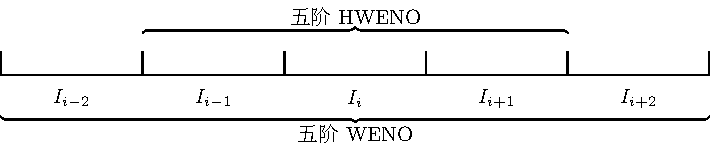
\includegraphics{fig/tikz/HWENO.pdf}
            \end{figure}
          }
          
    \item DG方法的空间离散也可以视为重构 \citep{DG-1989,DG-1990,DG-2016}
          
    \item $P_NP_M$方法 \citep{PNPM,luo2012hermite,xia2014implicit}
          
  \end{itemize}
  
\end{frame}

\begin{frame}{研究现状-解法器}
  
  \TextAndFig[0.7\textwidth]{
    \begin{itemize}[<+->]
      \item Godunov解法器 \citep{godunov}
            
      \item 局部线性化的Roe解法器 \citep{Roe}
            
            双激波近似的HLL解法器 \citep{HLL}
            
            双激波单接触间断近似的HLLC解法器 \citep{HLLC}
            
      \item 广义黎曼问题(GRP)解法器 \citep{GRPgeneral}
            
            推广到欧拉框架 \citep{GRPpolytropic}
            
            推广到任意气体状态方程 \citep{GRP}
            
            推广到二维 \citep{GRP_qi}
    \end{itemize}
  }{
    \begin{figure}[htbp]
      \centering
      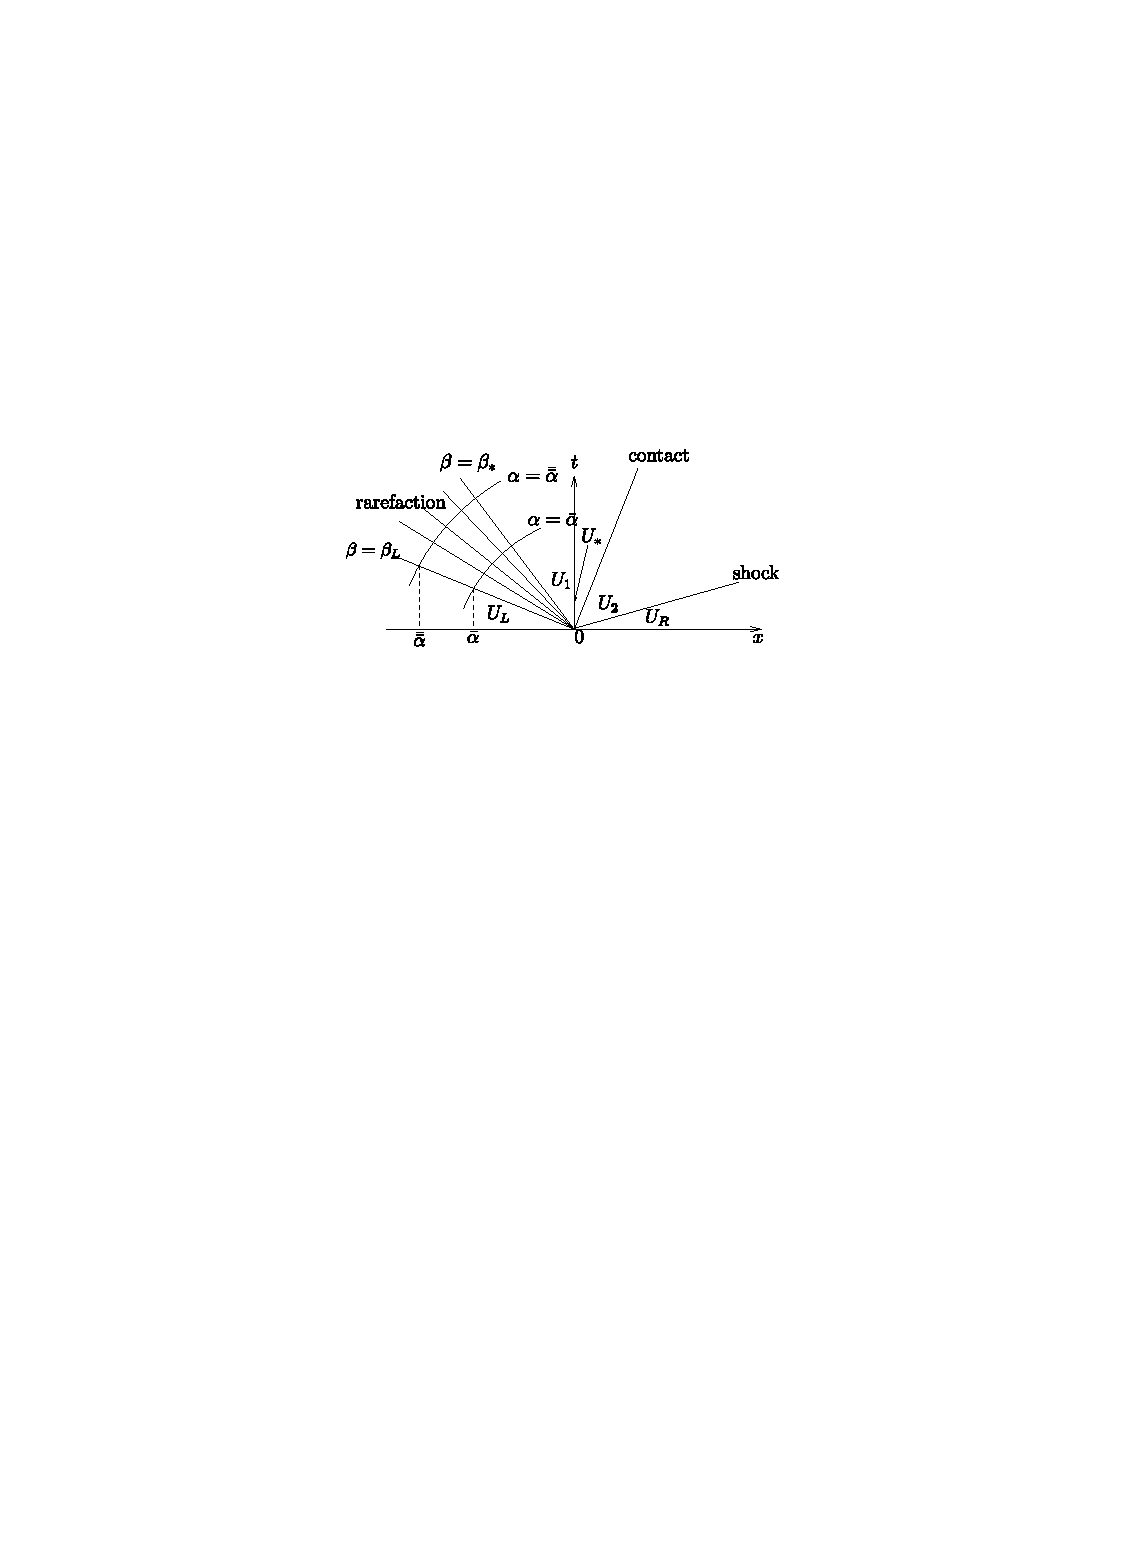
\includegraphics[width=\textwidth]{fig/RP_wave_pattern.pdf}
      \caption{黎曼问题}
    \end{figure}
    
    \onslide+<3>{
      \begin{figure}[htbp]
        \centering
        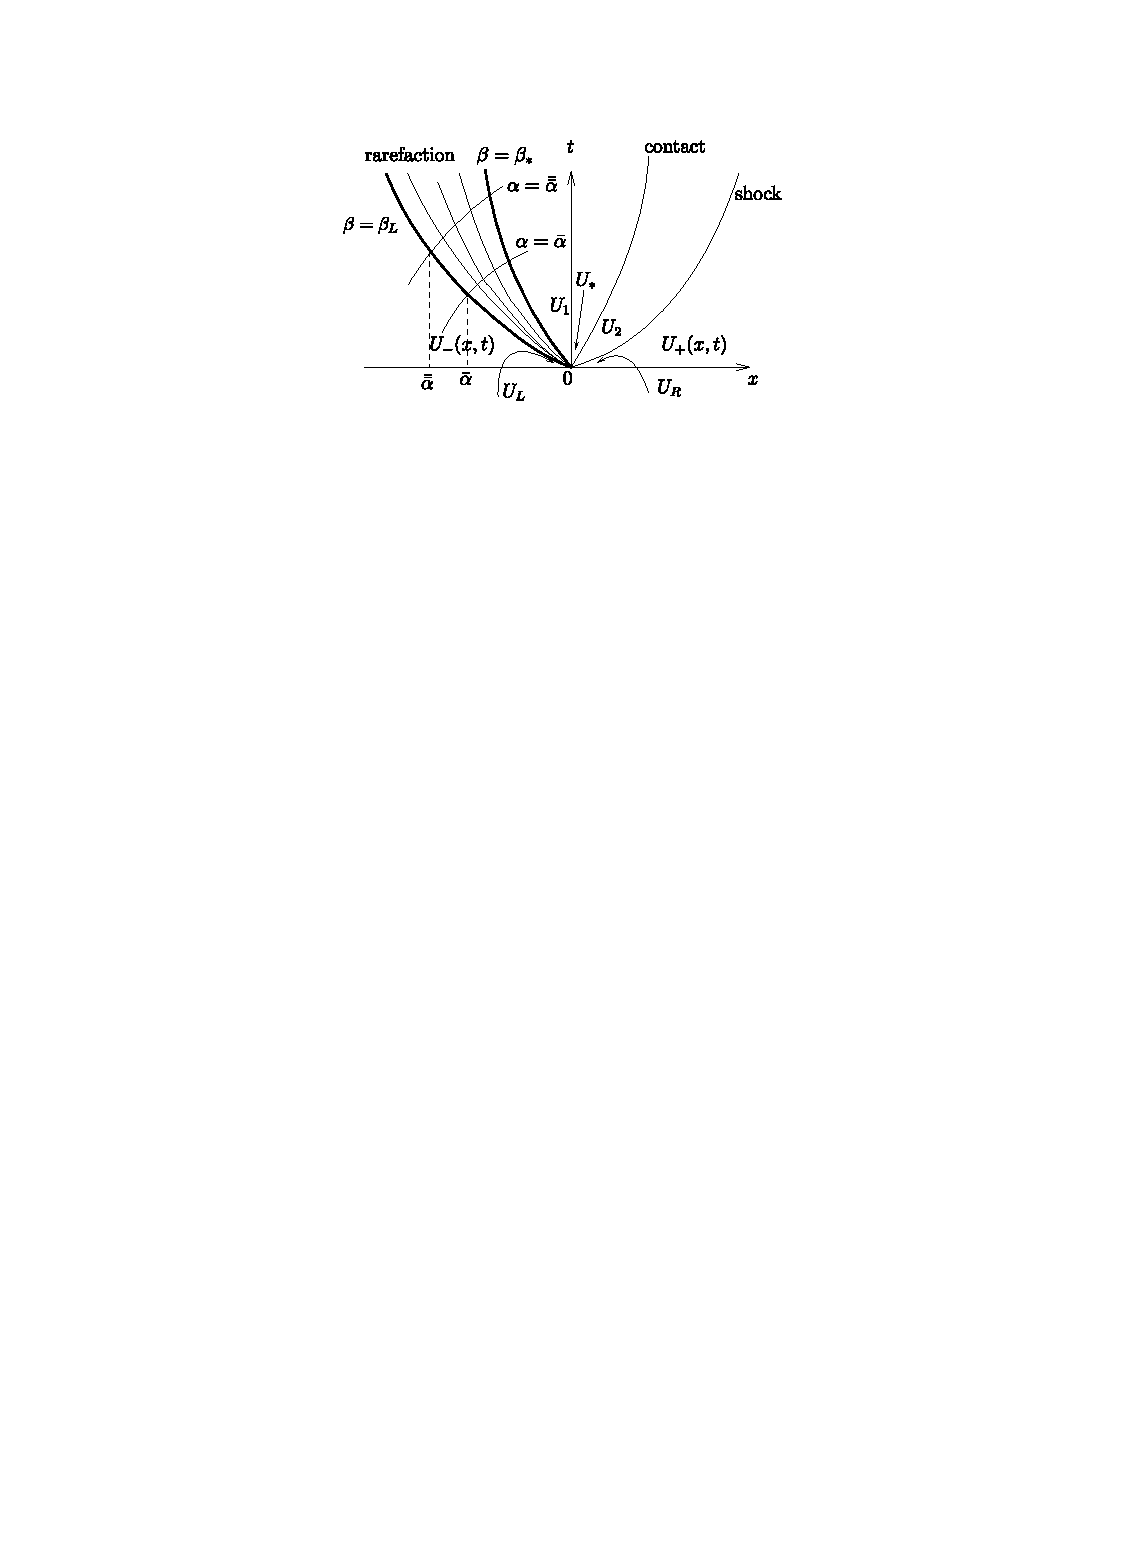
\includegraphics[width=\textwidth]{fig/GRP_wave_pattern.pdf}
        \caption{广义黎曼问题}
      \end{figure}
    }
  }
  
\end{frame}

\begin{frame}{研究动机}
  
  \begin{itemize}[<+->]
    \item 先前工作 \citep{du2018hermite} 中
          针对双曲守恒律,
          设计了一种两步四阶数值格式。
          基于HWENO5和WENO5重构以及GRP解法器。
          其中二维采用逐维重构。
          
    \item 为了进一步提高数值格式的\hl{紧致性},
          我们要研究求解双曲守恒律的基于紧致Hermite重构的显式两步四阶有限体积格式,
          即函数值和导数值\hl{均使用Hermite重构}获得。
          同时希望\hl{时空均是四阶精度的}。
          此外在二维情形下,
          我们要构造一个真正的二维重构,
          并设计相应的两步四阶格式。
  \end{itemize}
  
\end{frame}

\section{改进的双曲守恒律两步四阶时间推进框架}

\begin{frame}{原始的两步四阶时间推进框架}
  
  以线性对流方程为例:
  
  \begin{itemize}[<+->]
    \item 第一步
          \colorBOX{12cm}{-5mm}{-7mm}{
            \begin{align*}
              \bar{u}_{i}^{n+\frac 12}=\bar{u}_{i}^{n}-\frac{\tau}{2 h} \left(\hat{f}_{i+\frac 12}^*-\hat{f}_{i-\frac 12}^*\right), \quad
              \bar{v}_{i}^{n+\frac 12}=\frac{1}{h} \left(\hat u_{i+\frac 12}^{n+\frac 12}-\hat u_{i-\frac 12}^{n+\frac 12}\right),
            \end{align*}
          }
          \onslide*<1>{
            其中,
            \begin{align*}
              \label{eq:1D-s2-uhat}
              \hat{f}^*_{i+\frac{1}{2}}
               & ={f} \left(u_{i+\frac{1}{2}}^{n, +}\right) +\frac{\tau}{4} \left({\partial_{t}}{f}\right)_{i+\frac{1}{2}}^{n, +}=u_{i+\frac{1}{2}}^{n, +} +\frac{\tau}{4} \left({\partial_{t}}{u}\right)_{i+\frac{1}{2}}^{n, +}, \\
              \hat u_{i+\frac{1}{2}}^{n+\frac 12}
               & =u_{i+\frac{1}{2}}^{n, +}+\frac{\tau}{2} \left({\partial_{t}}u\right)_{i+\frac{1}{2}}^{n, +}.
            \end{align*}
          }
    \item 第二步
          \colorBOX{12cm}{-5mm}{-7mm}{
            \begin{align*}
              \bar{u}_{i}^{n+1}=\bar{u}_{i}^{n}-\frac{\tau}{ h} \left(\hat{f}_{i+\frac 12}^{4th}-\hat{f}_{i-\frac 12}^{4th}\right), \quad
              \bar{v}_{i}^{n+1}=\frac{1}{h} \left(\hat u_{i+\frac 12}^{n+1}-\hat u_{i-\frac 12}^{n+1}\right),
            \end{align*}
          }
          \onslide*<2>{
            其中,
            \begin{align*}
              \hat{f}^{4th}_{i+\frac{1}{2}}
               & ={f} \left(u_{i+\frac{1}{2}}^{n, +}\right) +\frac{\tau}{6} \left({\partial_{t}}{f}\right)_{i+\frac{1}{2}}^{n, +}+\frac{\tau}{3} \left({\partial_{t}}{f}\right)_{i+\frac{1}{2}}^{n+\frac12, +}
              =u_{i+\frac{1}{2}}^{n, +} +\frac{\tau}{6} \left({\partial_{t}}{u}\right)_{i+\frac{1}{2}}^{n, +}+\frac{\tau}{3} \left({\partial_{t}}{u}\right)_{i+\frac{1}{2}}^{n+\frac12, +},                     \\
              \hat u_{i+\frac{1}{2}}^{n+1}
               & =u_{i+\frac{1}{2}}^{n, +}+\tau \left({\partial_{t}}u\right)_{i+\frac{1}{2}}^{n+\frac{1}{2}, +}.
            \end{align*}
          }
  \end{itemize}
  
\end{frame}

\begin{frame}{需要改进的原因}
  
  \begin{itemize}[<+->]
    \item 为了设计基于紧致Hermite重构的显式两步四阶有限体积格式,
          首先构造\hl{恰好四阶精度}的紧致Hermite重构,
          再使用原始的两步四阶框架设计相应的格式。
          
    \item 然而,
          我们发现若函数值和导数值均使用(新构造的)Hermite重构,
          原始的两步四阶框架出现了\redhl{掉阶}。
  \end{itemize}
  
  \onslide<3>{\def\titleintable{CFL&$h$&Nstep&$L^1$-error&$L^1$-order&$L^\infty$-error&$L^\infty$-order\\}
\begin{table}[htbp]
  \caption{一维线性对流方程的精度测试中$u$的$L^1$和$L^\infty$误差和误差阶。}
  \centering
  \begin{tabular}{ccccccc}
    \toprule
    \titleintable
    \midrule
    0.6 & 2/40   & 34   & 1.38401e-05 &                 & 2.17751e-05 &                 \\
    0.6 & 2/80   & 67   & 1.73251e-06 & \redhl{2.99791} & 2.72250e-06 & \redhl{2.99967} \\
    0.6 & 2/160  & 134  & 2.17508e-07 & \redhl{2.99372} & 3.41695e-07 & \redhl{2.99415} \\
    0.6 & 2/320  & 267  & 2.72043e-08 & \redhl{2.99916} & 4.27335e-08 & \redhl{2.99927} \\
    0.6 & 2/640  & 534  & 3.40442e-09 & \redhl{2.99835} & 5.34770e-09 & \redhl{2.99838} \\
    0.6 & 2/1280 & 1067 & 4.25620e-10 & \redhl{2.99977} & 6.68734e-10 & \redhl{2.99942} \\
    \bottomrule
  \end{tabular}
\end{table}
\undef\titleintable}
  
\end{frame}

\begin{frame}{改进的过程:分析掉阶原因}
  
  \begin{itemize}[<+->]
    \item 以线性对流方程为例,
          利用泰勒展开,
          得到掉阶原因是$\bar v_{i}^{\frac 12}$的近似精度不够。
          所以需要将之提升至$\mathcal{O}(\tau^3)$,
          进而需要提高$\hat {u}^{\frac 12}_{i+\frac 12}$的精度。
          \begin{align*}
            \bar{v}_{i}^{n+\frac 12}=\frac{1}{h} \left(\hat u_{i+\frac 12}^{n+\frac 12}-\hat u_{i-\frac 12}^{n+\frac 12}\right), \quad
            \hat u_{i+\frac{1}{2}}^{n+\frac 12}
            =u_{i+\frac{1}{2}}^{n, +}+\frac{\tau}{2} \left({\partial_{t}}u\right)_{i+\frac{1}{2}}^{n, +}.
          \end{align*}
          
    \item 自然的,
          可以通过将泰勒展开增加一项来达到这个目标,
          即
          \colorBOX{10cm}{-3mm}{-7mm}{
            \begin{equation*}
              \hat u_{i+\frac{1}{2}}^{n+\frac 12}=u_{i+\frac{1}{2}}^{n, +}+\frac{\tau}{2} \left({\partial_{t}}u\right)_{i+\frac{1}{2}}^{n, +}+\HL{\frac{\tau^2}{8} \left({\partial_{t}^2}{u}\right)_{i+\frac{1}{2}}^{n, +}}.
            \end{equation*}
          }
          在此基础上,
          得到了改进的两步四阶时间推进框架。
  \end{itemize}
  
\end{frame}

\begin{frame}{改进的双曲守恒律两步四阶时间推进框架}
  
  \begin{equation*}
    \hat u_{i+\frac{1}{2}}^{n+\frac 12}=u_{i+\frac{1}{2}}^{n, +}+\frac{\tau}{2} \left({\partial_{t}}u\right)_{i+\frac{1}{2}}^{n, +}\onslide<2>{+\HL{\frac{\tau^2}{8} \left({\partial_{t}^2}{u}\right)_{i+\frac{1}{2}}^{n, +}}}
  \end{equation*}
  
  \begin{center}
    \begin{tabular}{ccccc}
      $u_{i+\frac{1}{2}}^{n, +}$
       & 
      $\stackrel{\textrm{需要}}{\longrightarrow}$
       & 
      Godunov解法器                                                             
       & 
      $\stackrel{\textrm{需要}}{\longrightarrow}$
       & 
      函数值重构
      \\[10mm]    
      
      $\left({\partial_{t}}u\right)_{i+\frac{1}{2}}^{n, +}$
       & 
      $\stackrel{\textrm{需要}}{\longrightarrow}$
       & 
      GRP解法器(一阶LW解法器)                                         
       & 
      $\stackrel{\textrm{需要}}{\longrightarrow}$
       & 
      导数值重构
      \\[10mm]    
      
      \onslide<2>{\HL{$\left({\partial_{t}^2}{u}\right)_{i+\frac{1}{2}}^{n, +}$}}
       & 
      \onslide<2>{\HL{$\stackrel{\textrm{需要}}{\longrightarrow}$}}
       & 
      \onslide<2>{\HL{线性近似的二阶LW解法器}}
       & 
      \onslide<2>{\HL{$\stackrel{\textrm{需要}}{\longrightarrow}$}}
       & 
      \onslide<2>{\HL{二阶导数值重构}}
      \\    
    \end{tabular}
  \end{center}
  
  \onslide<2>{
    \colorBOX{145mm}{0mm}{0mm}{
      在第一步时间推进中,
      改进的框架需要由二阶LW型解法器提供二阶时间导数。
      进而,
      需要重构算法提供二阶空间导数。
    }
  }
  
\end{frame}

\begin{frame}{改进的效果}
  
  \def\titleintable{CFL&$h$&Nstep&$L^1$-error&$L^1$-order&$L^\infty$-error&$L^\infty$-order\\}
% \begin{table}[htbp]
% 	\caption{HC-4格式在例 \ref{ex:1D-acc1} 中$u$的$L^1$和$L^\infty$误差和误差阶。展示的是$t^{tem} = 1$时刻的结果。}
% 	\label{ta:1D-ex1-HC4}
% 	\centering
% 	\begin{tabular}{ccccccc}
% 		\toprule
% 		\titleintable
% 		\midrule
% 		0.6 & 2/40   & 34   & 1.39581e-06 &              & 2.19020e-06 &              \\
% 		0.6 & 2/80   & 67   & 8.73170e-08 & \hl{3.99869} & 1.37118e-07 & \hl{3.99757} \\
% 		0.6 & 2/160  & 134  & 5.45979e-09 & \hl{3.99935} & 8.57559e-09 & \hl{3.99904} \\
% 		0.6 & 2/320  & 267  & 3.41097e-10 & \hl{4.00059} & 5.35806e-10 & \hl{4.00045} \\
% 		0.6 & 2/640  & 534  & 2.12972e-11 & \hl{4.00144} & 3.35383e-11 & \hl{3.99783} \\
% 		0.6 & 2/1280 & 1067 & 1.33043e-12 & \hl{4.00071} & 2.39120e-12 & \hl{3.81000} \\
% 		\bottomrule
% 	\end{tabular}
% \end{table}

\begin{table}[htbp]
	\caption{WHC-4格式在例 \ref{ex:1D-acc1} 中$u$的$L^1$和$L^\infty$误差和误差阶。展示的是$t^{tem} = 1$时刻的结果。}
	\label{ta:1D-ex1-WHC4}
	\centering
	\begin{tabular}{ccccccc}
		\toprule
		\titleintable
		\midrule
		0.6 & 2/40   & 34   & 1.39581e-06 &              & 2.19020e-06 &              \\
		0.6 & 2/80   & 67   & 8.73170e-08 & \hl{3.99869} & 1.37118e-07 & \hl{3.99757} \\
		0.6 & 2/160  & 134  & 5.45979e-09 & \hl{3.99935} & 8.57559e-09 & \hl{3.99904} \\
		0.6 & 2/320  & 267  & 3.41097e-10 & \hl{4.00059} & 5.35806e-10 & \hl{4.00045} \\
		0.6 & 2/640  & 534  & 2.12974e-11 & \hl{4.00143} & 3.35378e-11 & \hl{3.99785} \\
		0.6 & 2/1280 & 1067 & 1.33042e-12 & \hl{4.00072} & 2.38898e-12 & \hl{3.81132} \\
		\bottomrule
	\end{tabular}
\end{table}

\begin{table}[htbp]
	\caption{HHC-4格式在例 \ref{ex:1D-acc1} 中$u$的$L^1$和$L^\infty$误差和误差阶。展示的是$t^{tem} = 1$时刻的结果。}
	\label{ta:1D-ex1-HHC4}
	\centering
	\begin{tabular}{ccccccc}
		\toprule
		\titleintable
		\midrule
		0.6 & 2/40   & 34   & 1.39581e-06 &              & 2.19020e-06 &              \\
		0.6 & 2/80   & 67   & 8.73170e-08 & \hl{3.99869} & 1.37118e-07 & \hl{3.99757} \\
		0.6 & 2/160  & 134  & 5.45979e-09 & \hl{3.99935} & 8.57559e-09 & \hl{3.99904} \\
		0.6 & 2/320  & 267  & 3.41097e-10 & \hl{4.00059} & 5.35806e-10 & \hl{4.00045} \\
		0.6 & 2/640  & 534  & 2.12972e-11 & \hl{4.00144} & 3.35383e-11 & \hl{3.99783} \\
		0.6 & 2/1280 & 1067 & 1.33043e-12 & \hl{4.00071} & 2.39120e-12 & \hl{3.81000} \\
		\bottomrule
	\end{tabular}
\end{table}
\undef\titleintable
  
  \pause 二维也有类似的改进的两步四阶时间推进框架。
  
\end{frame}

\section[一维两步四阶数值格式]{一维基于紧致Hermite重构的双曲守恒律两步四阶数值格式}

\begin{frame}{一维基于紧致Hermite重构的双曲守恒律两步四阶数值格式}
  
  \begin{itemize}[<+->]
    \item 我们想要基于一维改进的两步四阶时间推进框架,
          设计一个两步四阶数值格式。
          
    \item 解法器:
          设计了一个线性二阶LW型解法器,
          同时采用Godunov解法器和GRP解法器。
          
    \item 重构:
          利用WENO和杂交选择技术,
          构造了两种四阶精度基本无振荡的非线性重构。
          
    \item 格式:
          设计了\hl{时空四阶精度基本无振荡的两步四阶格式},
          记作WHC-4和HHC-4格式。
          
    \item 格式:
          将上述格式推广到了空间八阶精度,
          记作WHC-8和HHC-8格式。
  \end{itemize}
  
\end{frame}

\subsection{广义黎曼问题解法器}

\begin{frame}{广义黎曼问题解法器}
  
  \begin{itemize}[<+->]
    \item Godunov解法器
          
    \item 文献 \citep{GRP} 中的GRP解法器
          
          \begin{itemize}
            \item 线性声波近似的 (acoustic) GRP 解法器
                  
            \item 非线性GRP解法器
          \end{itemize}
          
    \item 新设计的线性二阶LW型解法器
  \end{itemize}
  
  \onslide<5>{
    \colorBOX{13.5cm}{-6mm}{-7mm}{
      \begin{align*}
        \HL{{\partial_{t}^2} {\bm{u}}}
         & = -{\partial_{t}}{\partial_{x}}{\bm{f}}({\bm{u}})
        = -{\partial_{x}}\left(\frac{\partial{\bm{f}}}{\partial{\bm{u}}}({\bm{u}}) {\partial_{t}}{\bm{u}}\right)
        = -\frac{\partial^2{\bm{f}}}{\partial{\bm{u}}^2}({\bm{u}}) {\partial_{x}}{\bm{u}} {\partial_{t}}{\bm{u}}
        -\frac{\partial{\bm{f}}}{\partial{\bm{u}}}({\bm{u}}) \redHL{{\partial_{x}}{\partial_{t}}{\bm{u}}}, \\
        \redHL{{\partial_{x}}{\partial_{t}}{\bm{u}}}
         & = -{\partial_{x}}{\partial_{x}}{\bm{f}}({\bm{u}})
        = -{\partial_{x}}\left(\frac{\partial{\bm{f}}}{\partial{\bm{u}}}({\bm{u}}) {\partial_{x}}{\bm{u}}\right)
        = -\frac{\partial^2{\bm{f}}}{\partial{\bm{u}}^2}({\bm{u}}) {\partial_{x}}{\bm{u}} {\partial_{x}}{\bm{u}}
        -\frac{\partial{\bm{f}}}{\partial{\bm{u}}}({\bm{u}}) \HL{{\partial_{x}^2}{\bm{u}}}.
      \end{align*}
    }
  }
  
\end{frame}

\subsection{线性紧致Hermite重构及其相应的两步四阶格式}

\begin{frame}{一维Hermite重构}
  
  以均匀网格为例,
  给定未知函数$u(x)$的单元平均值和导数平均值
  \begin{equation*}
    \bar u_{i} = \frac {1}{h} \int_{I_{i}} u(x)dx, \quad
    \bar v_{i} = \frac {1}{h} \int_{I_{i}} v(x)dx = \frac{1}{h} (u(x_{i+\frac 12})-u(x_{i-\frac 12})), \quad
    i=1,\cdots, N,
  \end{equation*}
  重构给出插值多项式$p_{rj}(x)$,
  它定义在
  \begin{equation*}
    S^k_{r}(i) = \bigcup_{m=0}^{k-1} I_{i-r+m}, \quad
    r=0,1,\cdots, k-1, \quad
    k\ge 1,
  \end{equation*}
  上,
  并且满足
  \begin{equation*}
    {\partial_x^d}p^r_i(x) ={\partial_x^d} u(x) +\mathcal{O}(h^{2k-d}),\quad
    d=0,1,2.
  \end{equation*}
  
  \begin{figure}[htbp]
    \centering
    \begin{tikzpicture}[thick,scale=.3,line join=round,>=latex]
      \draw (0,0.5)--(0,0);
      \draw (6,0.5)--(6,0);
      \draw (12,0.5)--(12,0);
      \draw (18,0.5)--(18,0);
      \draw (24,0.5)--(24,0);
      \draw (30,0.5)--(30,0);
      \draw[->] (-3,0)--(33,0);
      \node at ( 3,1) {$I_{i-2}$};
      \node at ( 9,1) {$I_{i-1}$};
      \node at (15,1) {$I_{i  }$};
      \node at (21,1) {$I_{i+1}$};
      \node at (27,1) {$I_{i+2}$};
      \node at ( 0,-1) {$x_{i-\frac 52}$};
      \node at ( 6,-1) {$x_{i-\frac 32}$};
      \node at (12,-1) {$x_{i-\frac 12}$};
      \node at (18,-1) {$x_{i+\frac 12}$};
      \node at (24,-1) {$x_{i+\frac 32}$};
      \node at (30,-1) {$x_{i-\frac 52}$};
    \end{tikzpicture}
  \end{figure}
  
\end{frame}

\begin{frame}{线性紧致Hermite重构及其相应的两步四阶格式}
  
  \begin{itemize}[<+->]
    \only<3>{\setlength{\itemsep}{0mm}}
    \item 利用相邻2个单元中的4个信息,
          可以得到两个四阶线性重构。
          
          \onslide*<1,2>{
            \begin{figure}[htbp]
              \centering
              \begin{tikzpicture}[thick,scale=.3,line join=round,>=latex]
                \draw (0,0.5)--(0,0);
                \draw (6,0.5)--(6,0);
                \draw (12,0.5)--(12,0);
                \draw (18,0.5)--(18,0);
                \draw (24,0.5)--(24,0);
                \draw (30,0.5)--(30,0);
                \draw[->] (-3,0)--(33,0);
                \node at ( 3,1) {$I_{j-2}$};
                \node at ( 9,1) {$I_{j-1}$};
                \node at (15,1) {$I_{j  }$};
                \node at (21,1) {$I_{j+1}$};
                \node at (27,1) {$I_{j+2}$};
                \node at ( 0,-1) {$x_{j-\frac 52}$};
                \node at ( 6,-1) {$x_{j-\frac 32}$};
                \node at (12,-1) {$x_{j-\frac 12}$};
                \node at (18,-1) {$x_{j+\frac 12}$};
                \node at (24,-1) {$x_{j+\frac 32}$};
                \node at (30,-1) {$x_{j-\frac 52}$};
              \end{tikzpicture}
            \end{figure}
          }
          
    \item 使用改进的两步四阶时间推进框架,
          其中重构采用四阶线性重构,
          解法器采用GRP解法器,
          就得到了相应的两步四阶格式。
          
    \item 利用两值的线性稳定性分析,
          发现其中有一个稳定的\hl{线性紧致Hermite两步四阶格式},
          记作HC-4格式($k=2$)。
          
          \onslide*<3>{
            \vspace{-2mm}
            \begin{figure}[htbp]
              \centering
              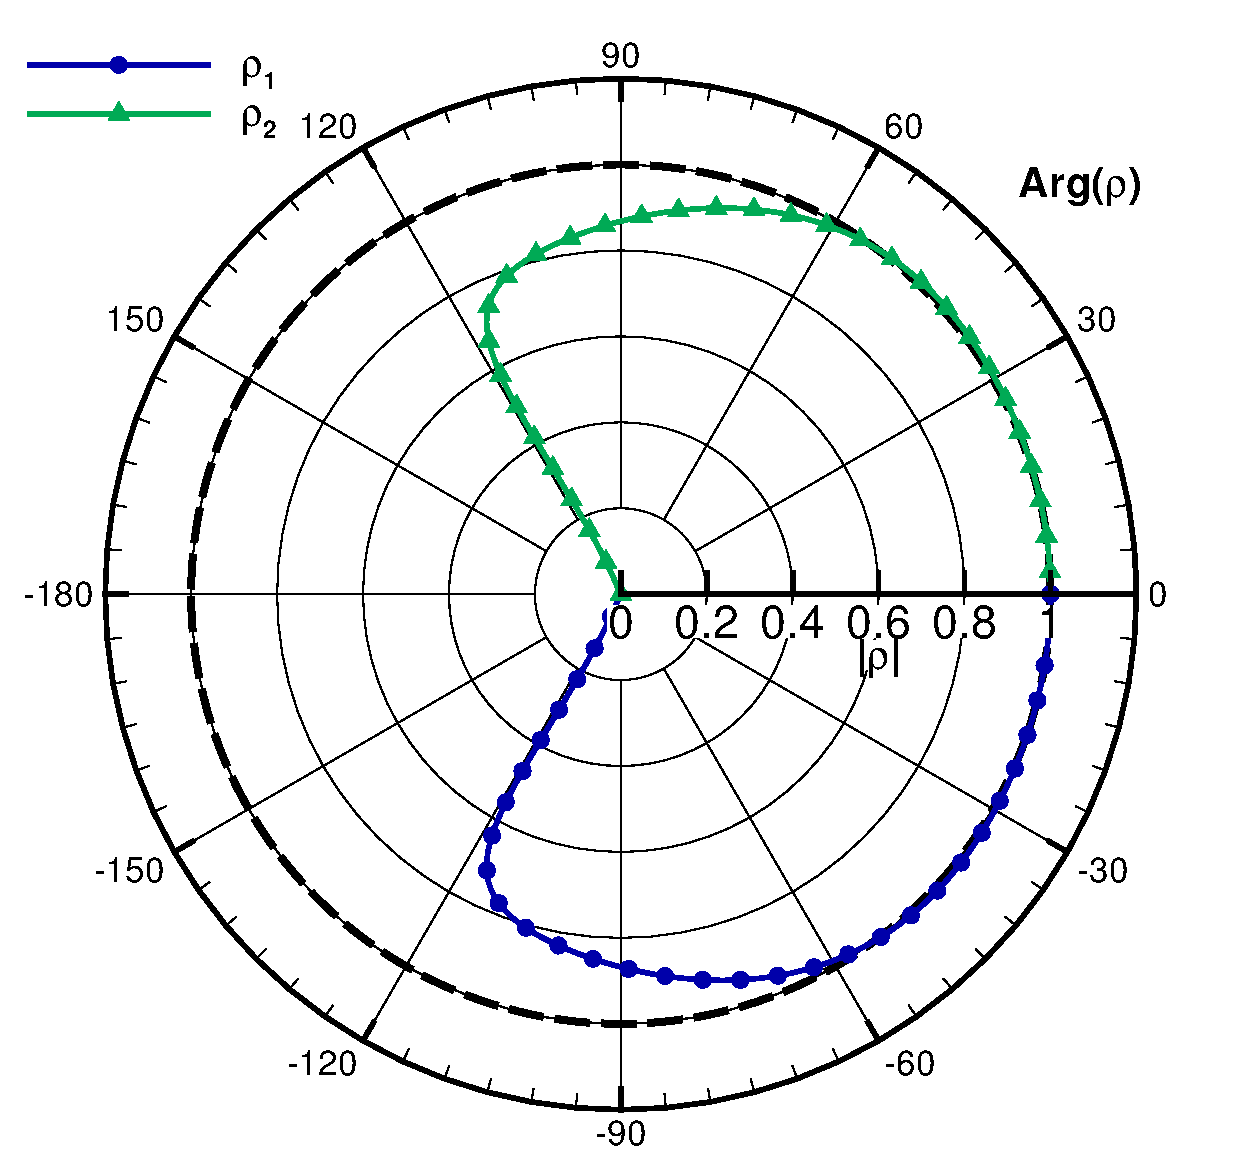
\includegraphics[width=0.33\textwidth]{fig/1D/pol40.pdf}
              \hspace{0.05\textwidth}
              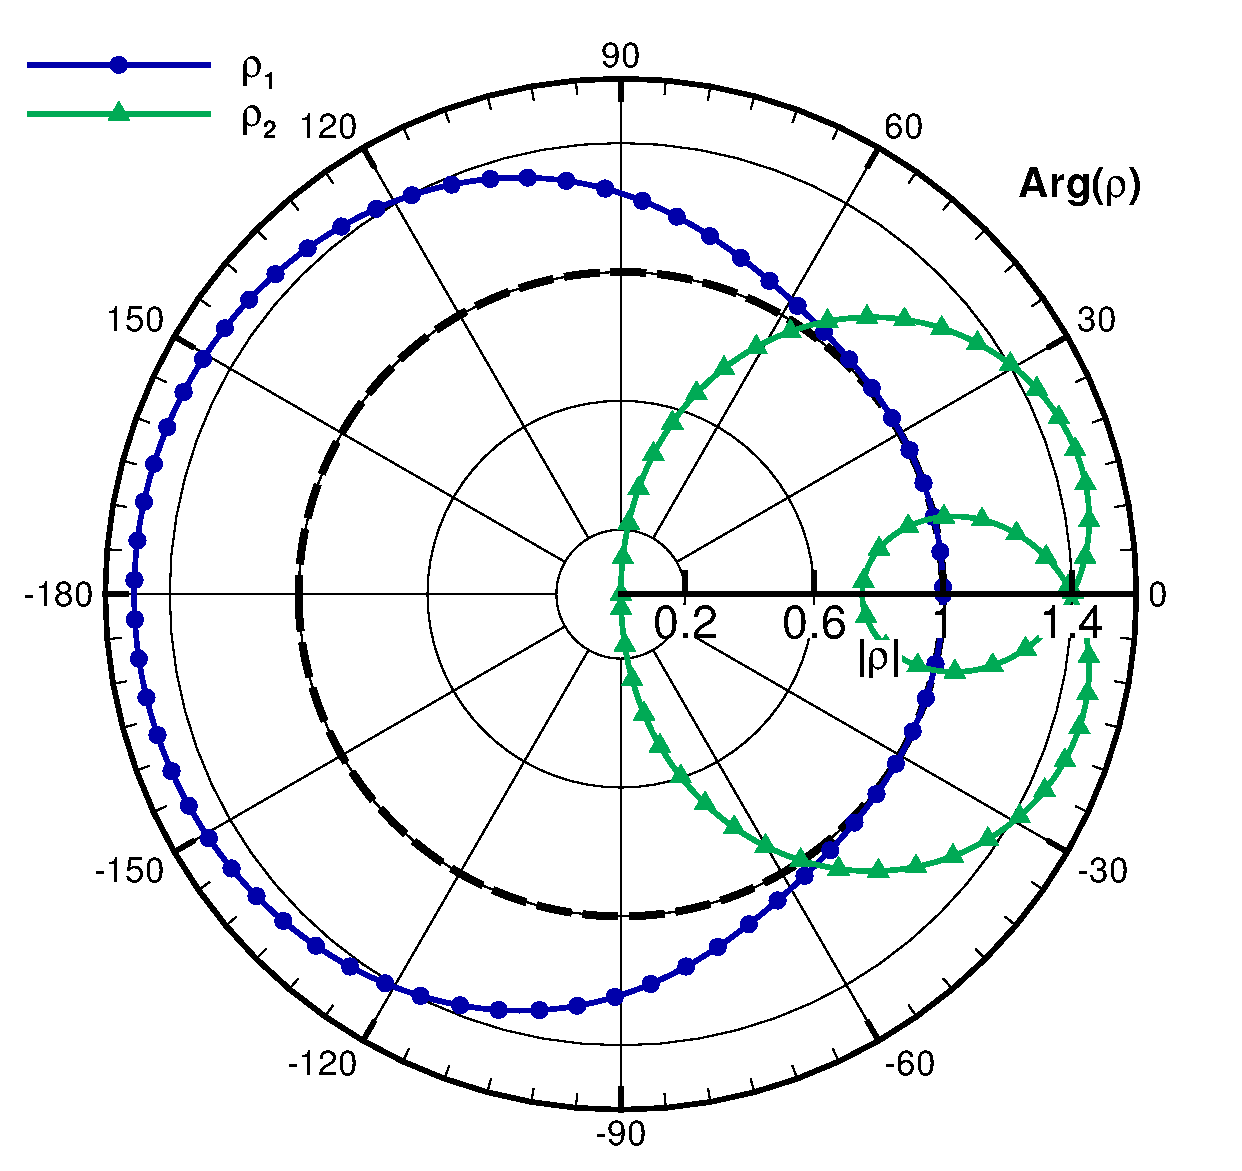
\includegraphics[width=0.33\textwidth]{fig/1D/pol41.pdf}
            \end{figure}
          }
          
    \item 类似的,有HC-2重构($k=1$)、HC-6格式($k=3$)和HC-8格式($k=4$)。
          
          \footnotesize HC代表埃尔米特构造(Hermite Construction)。
  \end{itemize}
  
\end{frame}

\subsection[非线性紧致Hermite重构及其相应的两步四阶格式]{基本无振荡的紧致Hermite重构及其相应的两步四阶格式}

\begin{frame}{加权型紧致Hermite重构(Weighted HC-4,WHC-4重构)}
  
  {
    \vspace{-2mm}
    \small
    参考 \citep{CWENO13579} 中的CWENO格式和 \citep{WENOAO} 中的WENO-AO格式。
    \vspace{2mm}
  }
  
  \begin{itemize}[<+->]
    \item 使用$k=1,2$两个线性重构作为组份,
          构造加权格式。
          将二阶和四阶重构的结果记为
          \begin{equation*}
            u_{i+\frac{1}{2},-}^{{o}}= p^{{o}}_{i}(x_{i+\frac{1}{2}}), \quad
            \left({\partial_{x}^{d}}u\right)_{i+\frac{1}{2},-}^{{o}}= {\partial_{x}^{d}}p_{i}^{{o}}(x_{i+\frac{1}{2}}), \quad d=1,2, \quad o=s,f.
          \end{equation*}
          
    \item 重写$u_{i+\frac{1}{2},-}^{{f}}$为
          \begin{equation*}
            u_{i+\frac{1}{2},-}^{{f}}= \gamma_{{s}}u_{i+\frac{1}{2},-}^{{s}}+ \gamma_{{f}}\left(\frac{1}{\gamma_{{f}}}u_{i+\frac{1}{2},-}^{{f}}-\frac{\gamma_{{s}}}{\gamma_{{f}}}u_{i+\frac{1}{2},-}^{{s}}\right), \quad \gamma_{{s}}+ \gamma_{{f}}=1.
          \end{equation*}
          
    \item 将线性权$\gamma_{{o}}$替换为非线性权$\omega_{{o}}$,
          \colorBOX{13cm}{-5mm}{-7mm}{
            \begin{align*}
              u_{i+\frac{1}{2},-}^{\text{WHC-4}}
               & = \HL{\omega_{{s}}}u_{i+\frac{1}{2},-}^{{s}}+ \HL{\omega_{{f}}}\left(\frac{1}{\gamma_{{f}}}u_{i+\frac{1}{2},-}^{{f}}-\frac{\gamma_{{s}}}{\gamma_{{f}}}u_{i+\frac{1}{2},-}^{{s}}\right), \quad \omega_{{s}}+\omega_{{f}}=1, \\
              \textrm{\kai{}即,\quad}
              u_{i+\frac{1}{2},-}^{\text{WHC-4}}
               & = \frac{\omega_{{f}}}{\gamma_{{f}}}u_{i+\frac{1}{2},-}^{{f}}+ \left(1-\frac{\omega_{{f}}}{\gamma_{{f}}}\right)u_{i+\frac{1}{2},-}^{{s}}.
            \end{align*}
          }
  \end{itemize}
  
\end{frame}

\begin{frame}{加权型紧致Hermite重构(Weighted HC-4,WHC-4重构)}
  
  \begin{itemize}[<+->]
    \item 非线性权的定义方式参考文献 \citep{WENO_Z} 中的WENO-Z格式:
          \begin{equation*}
            \omega_{{o}}=\frac{\alpha_{{o}}}{\alpha_{{s}}+\alpha_{{f}}}, \quad
            \alpha_{{o}}=\gamma_{{o}}\left( 1+\left( \frac{\theta}{\beta_{{o}}+\varepsilon}\right)^q \right) , \quad {{o}}={{s}}, {{f}},
          \end{equation*}
          其中,
          $\theta = |\beta_{{s}}-\beta_{{f}}|$,$\varepsilon=\widehat{C}h^3$,$\widehat{C}=100$,$q = 2$.
          
    \item 光滑因子$\beta_{{s}}$和$\beta_{{f}}$参考文献 \citep{WENO-1996} 中的定义:
          \begin{equation*}
            \beta_{{o}}= \sum_{d=1}^3 \int_{I_{i}}h^{2\ell-1}\left({\partial_{x}^{d}}p^{{o}}_{i}(x)\right)^2 dx, \quad {{o}}={{s}},{{f}}.
          \end{equation*}
          
    \item 使用相同的非线性权可以得到一阶和二阶空间导数:
          \colorBOX{12cm}{-5mm}{-7mm}{
            \begin{equation*}
              \left({\partial_{x}^{d}}u\right)_{i+\frac{1}{2},-}^{\text{WHC-4}}= \frac{\omega_{{f}}}{\gamma_{{f}}}\left({\partial_{x}^{d}}u\right)_{i+\frac{1}{2},-}^{{f}}+ \left(1-\frac{\omega_{{f}}}{\gamma_{{f}}}\right)\left({\partial_{x}^{d}}u\right)_{i+\frac{1}{2},-}^{{s}}, \quad d=1,2.
            \end{equation*}
          }
  \end{itemize}
  
\end{frame}

\begin{frame}{WHC-4重构的性质}
  
  \begin{itemize}[<+->]
    \item 非线性权在光滑区域内满足以下关系
          \begin{equation*}
            \omega_{{o}}= \gamma_{{o}}+ {\mathcal{O}}(h^2) , \quad {{o}}={{s}}, {{f}}.
          \end{equation*}
          
    \item 因此,
          $u_{i+\frac{1}{2},-}^{\text{WHC-4}}$是对精确值$u(x_{i+\frac{1}{2}})$的四阶精确近似:
          \begin{equation*}
            u_{i+\frac{1}{2},-}^{\text{WHC-4}}= u_{i+\frac{1}{2},-}^{{f}}+ \frac{\omega_{{f}}- \gamma_{{f}}}{\gamma_{{f}}}\left(u_{i+\frac{1}{2},-}^{{f}}-u_{i+\frac{1}{2},-}^{{s}}\right) = u_{i+\frac{1}{2},-}^{{f}}+ {\mathcal{O}}(h^4)= u(x_{i+\frac{1}{2}})+{\mathcal{O}}(h^4).
          \end{equation*}
          
    \item 在间断附近:
          \begin{equation*}
            \omega_{{s}}= 1-{\mathcal{O}}(h^4), \quad \omega_{{f}}= {\mathcal{O}}(h^4),
          \end{equation*}
          使得带有minmod限制器的二阶重构起主要作用,
          从而可有效防止振荡。 
  \end{itemize}
  
\end{frame}

\begin{frame}{杂交选择型紧致Hermite重构(Hybrid HC-4,HHC-4重构)}
  
  \begin{itemize}[<+->]
    \item 第一项的系数${\omega_{{f}}}/{\gamma_{{f}}}$在光滑区域趋近于$1$,
          在间断附近趋近于$0$。
          \begin{equation*}
            u_{i+\frac{1}{2},-}^{\text{WHC-4}}= \frac{\omega_{{f}}}{\gamma_{{f}}}u_{i+\frac{1}{2},-}^{{f}}+ \left(1 - \frac{\omega_{{f}}}{\gamma_{{f}}}\right) {u}_{i+\frac{1}{2},-}^{{s}}.
          \end{equation*}
          
    \item 因此,
          我们可以应用一个截断函数,
          得到我们的杂交选择型重构
          \begin{equation*}
            \label{eq:1D-HHC4-perpare}
            u_{i+\frac{1}{2},-}^{\text{HHC-4}}= \delta\left(\frac{\omega_{{f}}}{\gamma_{{f}}}\right) u_{i+\frac{1}{2},-}^{{f}}+ \left(1-\delta\left(\frac{\omega_{{f}}}{\gamma_{{f}}}\right) \right) {u}_{i+\frac{1}{2},-}^{{s}}.
          \end{equation*}
          
    \item 选择恰当的截断函数并整理不等式,得到
          \colorBOX{10cm}{-2mm}{-5mm}{
            \begin{equation*}
              \label{eq:1D-HHC4}
              \begin{aligned}
                u_{i+\frac{1}{2},-}^{\text{HHC-4}}=
                \begin{cases}
                  u_{i+\frac{1}{2},-}^{{f}}, & \beta_{{f}}+\varepsilon < \HL{\bar{\vartheta}}(\beta_{{s}}+\varepsilon),    \\
                  u_{i+\frac{1}{2},-}^{{s}}, & \beta_{{f}}+\varepsilon \ge \HL{\bar{\vartheta}}(\beta_{{s}}+\varepsilon),
                \end{cases}
                \quad\quad
                \bar{\vartheta} = 50.
              \end{aligned}
            \end{equation*}
          }
  \end{itemize}
  
\end{frame}

\begin{frame}{WHC-4和HHC-4格式及其紧致性}
  
  使用改进的两步四阶时间推进框架,
  其中重构采用WHC-4和HHC-4重构,
  解法器采用GRP解法器,
  就得到了相应的两步四阶格式。  
  
  \begin{figure}[htbp]
    \centering
    \subfigure[WHC-4和HHC-4格式的数值通量的依赖区域]{
      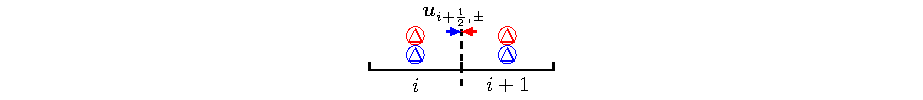
\includegraphics{fig/tikz/compact-1D-flux.pdf}
    } \\
    \footnotesize 标记${\bigcirc}$代表单元平均值,
    标记${\Delta}$代表导数平均值。\\
    {\color{blue}蓝色}代表左侧重构值的依赖范围,
    而{\color{red}红色}代表右侧重构值的依赖范围。\\
    \subfigure[WHC-4和HHC-4格式的依赖区域]{
      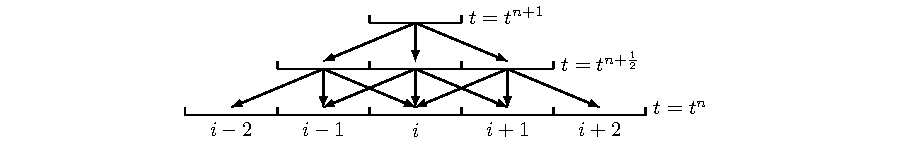
\includegraphics{fig/tikz/compact-1D-HC4.pdf}
    }
  \end{figure}
  
\end{frame}

\begin{frame}{WHC-4和HHC-4格式及其紧致性}
  
  \vspace{-1cm}
  \begin{figure}[htbp]
    \centering
    \subfigure[文献 \citep{du2018hermite} 中的S2O4-HWENO5格式的数值通量的依赖区域。]{
      \label{subfig:flux2}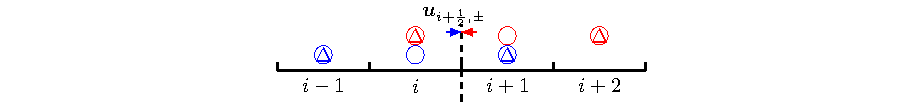
\includegraphics{fig/tikz/compact-1D-flux2.pdf}
    } \\
    \footnotesize 标记${\bigcirc}$代表单元平均值,
    标记${\Delta}$代表导数平均值。\\
    {\color{blue}蓝色}代表左侧重构值的依赖范围,
    而{\color{red}红色}代表右侧重构值的依赖范围。\\
    \subfigure[文献 \citep{du2018hermite} 中的S2O4-HWENO5格式的依赖区域]{
      \label{subfig:1D-compact-HWENO5}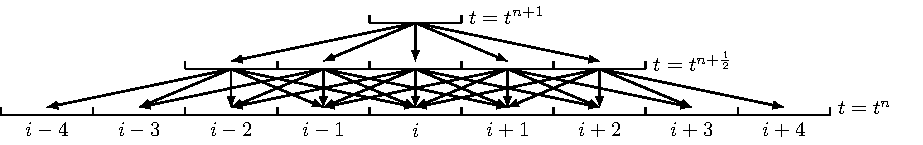
\includegraphics{fig/tikz/compact-1D-HWENO5.pdf}
    }
  \end{figure}
  
\end{frame}

\subsection{数值实验}

\begin{frame}{一维欧拉方程组的线性退化的精度测试}
  
  \begin{example}[一维欧拉方程组的线性退化的精度测试]
    \label{ex:1D-acc2}
    这个算例选择欧拉方程组
    \begin{equation*}
      \label{eq:1D-Euler}
      {\partial_{t}}{\bm{u}} + {\partial_{x}}{\bm{f}}({\bm{u}}) = 0, \quad
      {\bm{u}} =(\rho, \rho u, \rho E)^\top, \quad
      {\bm{f}}({\bm{u}}) =(\rho u,\rho u^2+p, u(\rho E+p))^\top,
    \end{equation*}
    作为模型,
    其中多方指数$\gamma$取$1.4$,
    初值为
    \begin{equation*}
      \rho(x, 0) = 1 + 0.2\sin(\pi x), \quad u(x,0)=1, \quad p(x,0)=1.
    \end{equation*}
    计算区域是$[-1,1]$,
    采取周期边界条件。
    这个问题的精确解是${\bm{u}}(x,t) = {\bm{u}}(x-t,0)$。
  \end{example}
  
\end{frame}

\begin{frame}{一维欧拉方程组的线性退化的精度测试结果}
  
  \vspace{-3mm}
  \begin{columns}
    \begin{column}{0.2\textwidth}
      
      \centering
      
      WHC-4格式
      
      \vspace{0.4\textheight}
      
      HHC-4格式
      
    \end{column}
    \begin{column}{0.8\textwidth}
      \begin{small}
        \def\titleintable{CFL&$h$&Nstep&$L^1$-error&$L^1$-order&$L^\infty$-error&$L^\infty$-order\\}
% \begin{table}[htbp]
%   \caption{HC-4格式在例 \ref{ex:1D-acc2} 中密度的$L^1$和$L^\infty$误差和误差阶。展示的是$t^{tem} = 10$时刻的结果。}
%   \label{ta:1D-ex2-HC4}
%   \centering
%   \begin{tabular}{ccccccc}
%     \toprule
%     \titleintable
%     \midrule
%     0.6 & 2/40   & 775   & 1.35453e-05 &         & 2.12772e-05 &         \\
%     0.6 & 2/80   & 1549  & 8.46534e-07 & 4.00009 & 1.32973e-06 & 4.00010 \\
%     0.6 & 2/160  & 3098  & 5.29071e-08 & 4.00003 & 8.31064e-08 & 4.00003 \\
%     0.6 & 2/320  & 6195  & 3.30668e-09 & 4.00001 & 5.19407e-09 & 4.00002 \\
%     0.6 & 2/640  & 12389 & 2.06655e-10 & 4.00008 & 3.25390e-10 & 3.99663 \\
%     0.6 & 2/1280 & 24778 & 1.29157e-11 & 4.00003 & 2.19097e-11 & 3.89253 \\
%     \bottomrule
%   \end{tabular}
% \end{table}

\begin{table}[htbp]
  % \caption{WHC-4格式在例 \ref{ex:1D-acc2} 中密度的$L^1$和$L^\infty$误差和误差阶。展示的是$t^{tem} = 10$时刻的结果。}
  \label{ta:1D-ex2-WHC4}
  \centering
  \begin{tabular}{ccccccc}
    \toprule
    \titleintable
    \midrule
    0.6 & 2/40   & 775   & 1.35453e-05 &              & 2.12772e-05 &              \\
    0.6 & 2/80   & 1549  & 8.46533e-07 & \hl{4.00009} & 1.32973e-06 & \hl{4.00010} \\
    0.6 & 2/160  & 3098  & 5.29071e-08 & \hl{4.00003} & 8.31064e-08 & \hl{4.00003} \\
    0.6 & 2/320  & 6195  & 3.30668e-09 & \hl{4.00001} & 5.19407e-09 & \hl{4.00002} \\
    0.6 & 2/640  & 12389 & 2.06656e-10 & \hl{4.00008} & 3.25396e-10 & \hl{3.99660} \\
    0.6 & 2/1280 & 24778 & 1.29151e-11 & \hl{4.00010} & 2.18940e-11 & \hl{3.89359} \\
    \bottomrule
  \end{tabular}
\end{table}

\begin{table}[htbp]
  % \caption{HHC-4格式在例 \ref{ex:1D-acc2} 中密度的$L^1$和$L^\infty$误差和误差阶。展示的是$t^{tem} = 10$时刻的结果。}
  \label{ta:1D-ex2-HHC4}
  \centering
  \begin{tabular}{ccccccc}
    \toprule
    \titleintable
    \midrule
    0.6 & 2/40   & 775   & 1.35453e-05 &              & 2.12772e-05 &              \\
    0.6 & 2/80   & 1549  & 8.46534e-07 & \hl{4.00009} & 1.32973e-06 & \hl{4.00010} \\
    0.6 & 2/160  & 3098  & 5.29071e-08 & \hl{4.00003} & 8.31064e-08 & \hl{4.00003} \\
    0.6 & 2/320  & 6195  & 3.30668e-09 & \hl{4.00001} & 5.19407e-09 & \hl{4.00002} \\
    0.6 & 2/640  & 12389 & 2.06659e-10 & \hl{4.00008} & 3.25382e-10 & \hl{3.99669} \\
    0.6 & 2/1280 & 24778 & 1.29121e-11 & \hl{4.00043} & 2.19050e-11 & \hl{3.89280} \\
    \bottomrule
  \end{tabular}
\end{table}
\undef\titleintable
      \end{small}
    \end{column}
  \end{columns}
  
\end{frame}

\begin{frame}{一维欧拉方程组的非线性的精度测试}
  
  \begin{example}[一维欧拉方程组的非线性的精度测试]
    \label{ex:1D-acc3}
    这是一个源自文献 \citep{Gamma3-HWENO} 的数值算例,
    初始条件设定为
    \begin{equation*}
      \rho(x, 0)=\frac{1+0.2x}{\sqrt{12}}, \quad
      u(x, 0)=\sqrt{\gamma}\rho(x, y, 0), \quad
      p(x, 0)=\rho(x, 0)^\gamma.
    \end{equation*}
    计算区域是$[0, 2\pi]$,
    并且使用与例 \ref{ex:1D-acc2} 相同的
    欧拉方程组、均匀网格和周期边界。
    不过,
    多方指数$\gamma$设定为3。
  \end{example}
  
\end{frame}

\begin{frame}{一维欧拉方程组的非线性的精度测试结果}
  
  \vspace{-3mm}
  \begin{columns}
    \begin{column}{0.2\textwidth}
      
      \centering
      
      WHC-4格式
      
      \vspace{0.4\textheight}
      
      HHC-4格式
      
    \end{column}
    \begin{column}{0.8\textwidth}
      \begin{small}
        \def\titleintable{CFL&$h$&Nstep&$L^1$-error&$L^1$-order&$L^\infty$-error&$L^\infty$-order\\}
\begin{table}[htbp]
  \caption{HC-4格式在\cref{ex:2D-acc3} 中$u$的$L^1$和$L^\infty$误差和误差阶。展示的是$t^{tem} = 1$时刻的结果。}
  \label{ta:2D-ex3-HC4}
  \centering
  \begin{tabular}{ccccccc}
    \toprule
    \titleintable
    \midrule
    % 0.6 &$4\pi$/100 & 32 & 1.03900e-07 & & 4.49257e-07 & \\
    % 0.6 &$4\pi$/150 & 48 & 2.10901e-08 & 3.93283 & 1.11949e-07 & 3.42706 \\
    0.6 & $4\pi$/150 & 48  & 2.10901e-08 &         & 1.11949e-07 &         \\
    0.6 & $4\pi$/200 & 64  & 6.84370e-09 & 3.91221 & 3.00975e-08 & 4.56615 \\
    0.6 & $4\pi$/250 & 80  & 2.80492e-09 & 3.99723 & 1.23554e-08 & 3.99003 \\
    0.6 & $4\pi$/300 & 96  & 1.35184e-09 & 4.00341 & 5.97173e-09 & 3.98776 \\
    0.6 & $4\pi$/350 & 112 & 7.29333e-10 & 4.00316 & 3.23427e-09 & 3.97815 \\
    0.6 & $4\pi$/400 & 128 & 4.27356e-10 & 4.00290 & 1.91305e-09 & 3.93243 \\
    \bottomrule
  \end{tabular}
\end{table}

\begin{table}[htbp]
  \caption{WHC-4格式在\cref{ex:2D-acc3} 中$u$的$L^1$和$L^\infty$误差和误差阶。展示的是$t^{tem} = 1$时刻的结果。}
  \label{ta:2D-ex3-WHC4}
  \centering
  \begin{tabular}{ccccccc}
    \toprule
    \titleintable
    \midrule
    % 0.6 &$4\pi$/100 & 32 & 1.03900e-07 & & 4.49257e-07 & \\
    % 0.6 &$4\pi$/150 & 48 & 2.10901e-08 & 3.93283 & 1.11949e-07 & 3.42706 \\
    0.6 & $4\pi$/150 & 48  & 2.10901e-08 &         & 1.11949e-07 &         \\
    0.6 & $4\pi$/200 & 64  & 6.84370e-09 & 3.91221 & 3.00975e-08 & 4.56615 \\
    0.6 & $4\pi$/250 & 80  & 2.80492e-09 & 3.99723 & 1.23554e-08 & 3.99003 \\
    0.6 & $4\pi$/300 & 96  & 1.35184e-09 & 4.00341 & 5.97173e-09 & 3.98776 \\
    0.6 & $4\pi$/350 & 112 & 7.29333e-10 & 4.00316 & 3.23427e-09 & 3.97815 \\
    0.6 & $4\pi$/400 & 128 & 4.27356e-10 & 4.00290 & 1.91305e-09 & 3.93243 \\
    \bottomrule
  \end{tabular}
\end{table}

\begin{table}[htbp]
  \caption{HHC-4格式在\cref{ex:2D-acc3} 中$u$的$L^1$和$L^\infty$误差和误差阶。展示的是$t^{tem} = 1$时刻的结果。}
  \label{ta:2D-ex3-HHC4}
  \centering
  \begin{tabular}{ccccccc}
    \toprule
    \titleintable
    \midrule
    % 0.6 &$4\pi$/100 & 32 & 1.03900e-07 & & 4.49257e-07 & \\
    % 0.6 &$4\pi$/150 & 48 & 2.10901e-08 & 3.93283 & 1.11949e-07 & 3.42706 \\
    0.6 & $4\pi$/150 & 48  & 2.10901e-08 &         & 1.11949e-07 &         \\
    0.6 & $4\pi$/200 & 64  & 6.84370e-09 & 3.91221 & 3.00975e-08 & 4.56615 \\
    0.6 & $4\pi$/250 & 80  & 2.80492e-09 & 3.99723 & 1.23554e-08 & 3.99003 \\
    0.6 & $4\pi$/300 & 96  & 1.35184e-09 & 4.00341 & 5.97173e-09 & 3.98776 \\
    0.6 & $4\pi$/350 & 112 & 7.29333e-10 & 4.00316 & 3.23427e-09 & 3.97815 \\
    0.6 & $4\pi$/400 & 128 & 4.27356e-10 & 4.00290 & 1.91305e-09 & 3.93243 \\
    \bottomrule
  \end{tabular}
\end{table}
\undef\titleintable
      \end{small}
    \end{column}
  \end{columns}
  
\end{frame}

% \begin{frame}{一维欧拉方程组的含间断问题}

%   \begin{figure}[htbp]
%     \centering
%     \subfigure[Lax激波管问题]{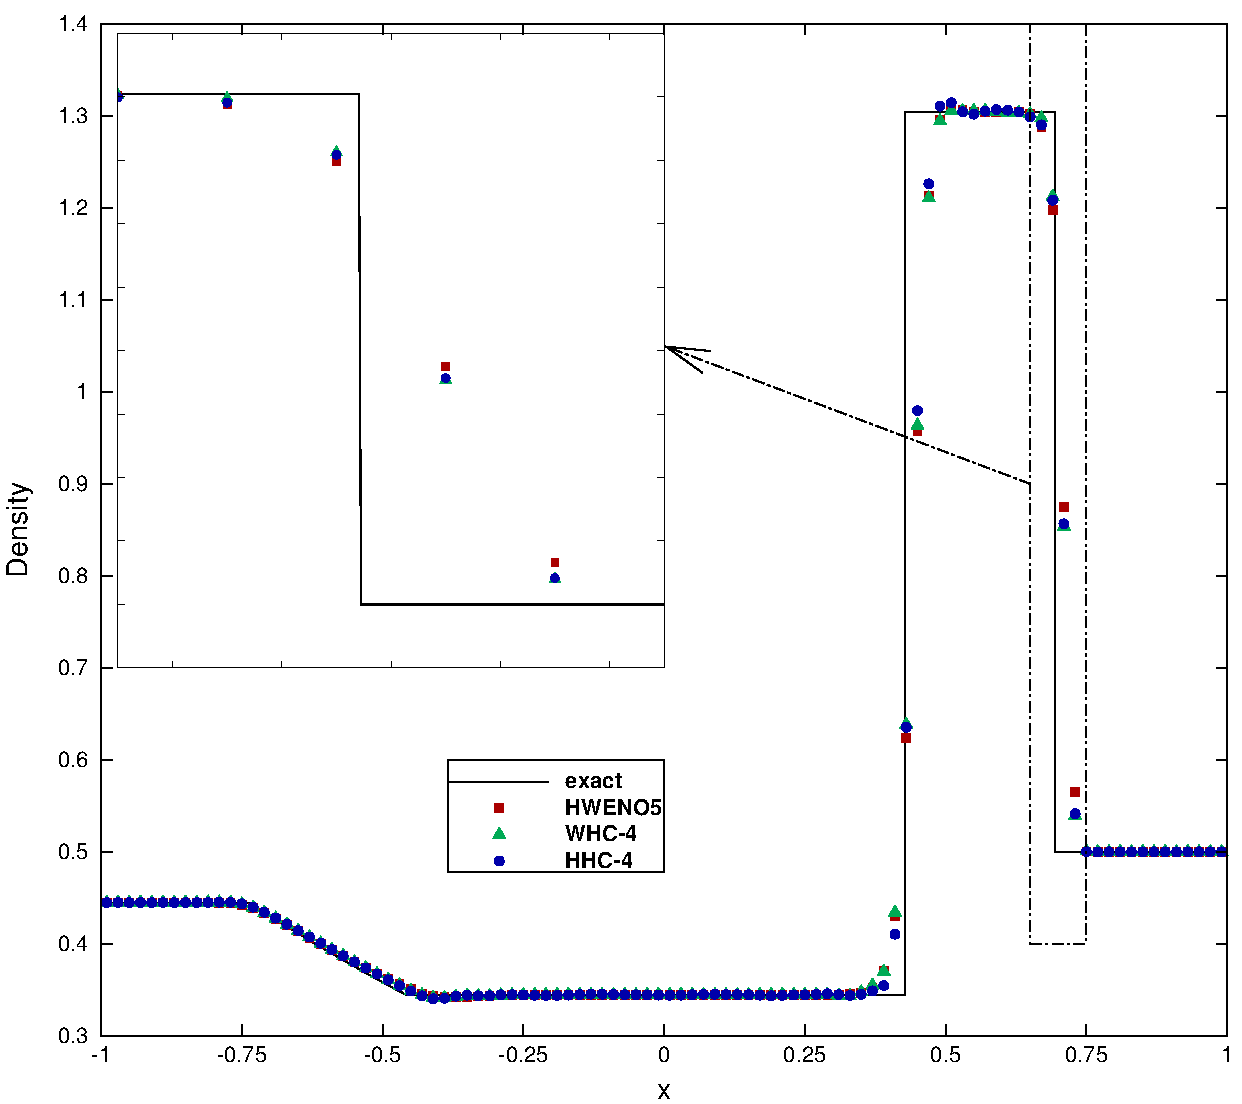
\includegraphics[height=0.33\textheight]{fig/1D/Ex2.pdf}}
%     \hspace{10mm}
%     \subfigure[Shu-Osher问题]{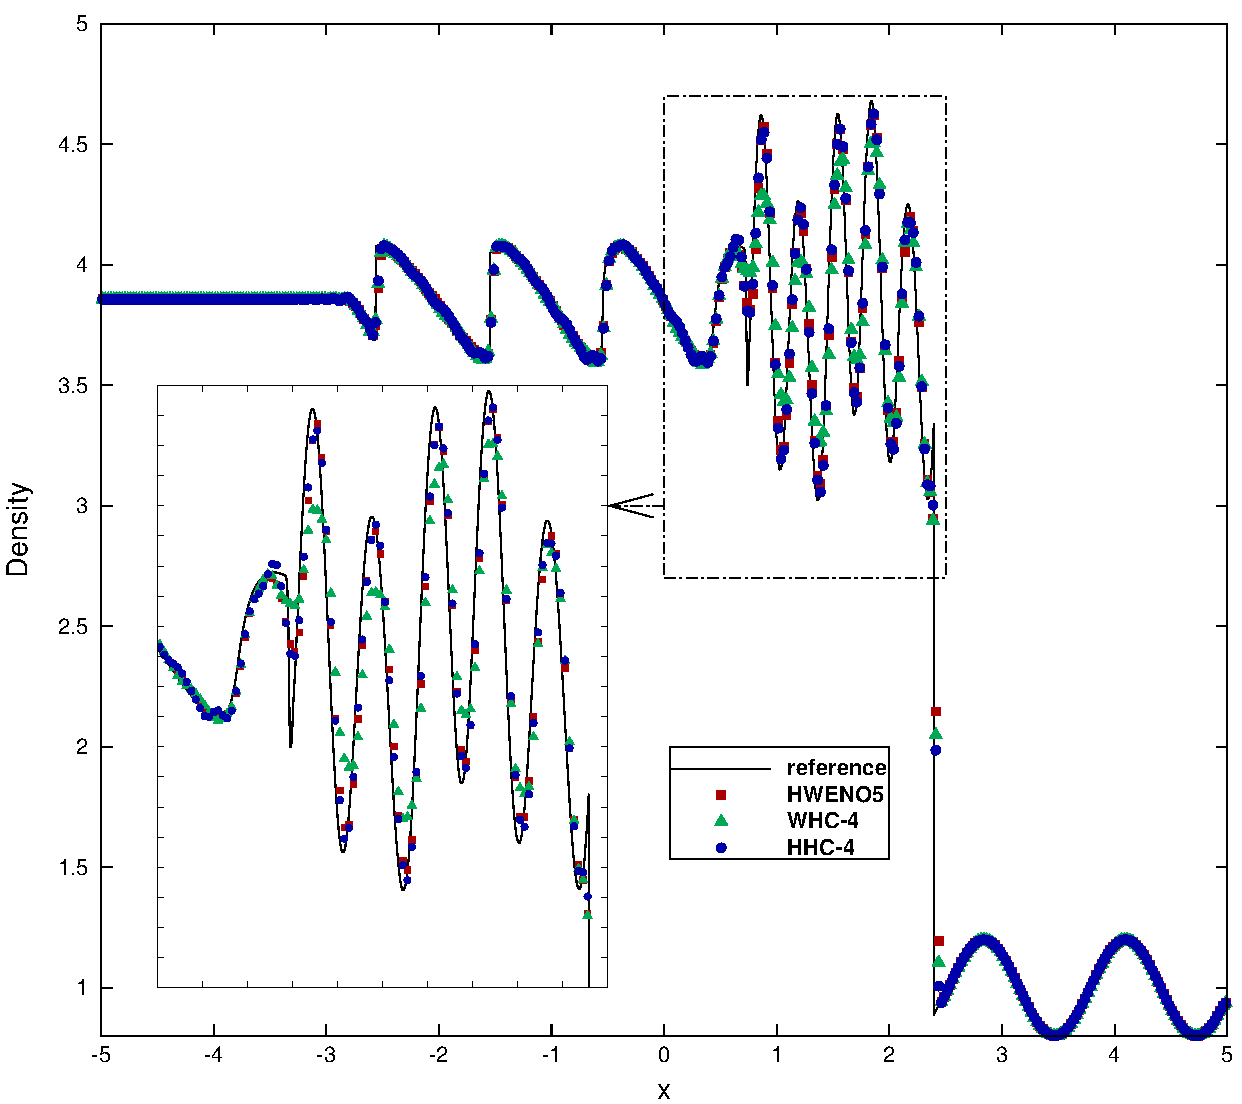
\includegraphics[height=0.33\textheight]{fig/1D/Ex3.pdf}}
%     \hspace{10mm}
%     \subfigure[Titarev-Toro问题]{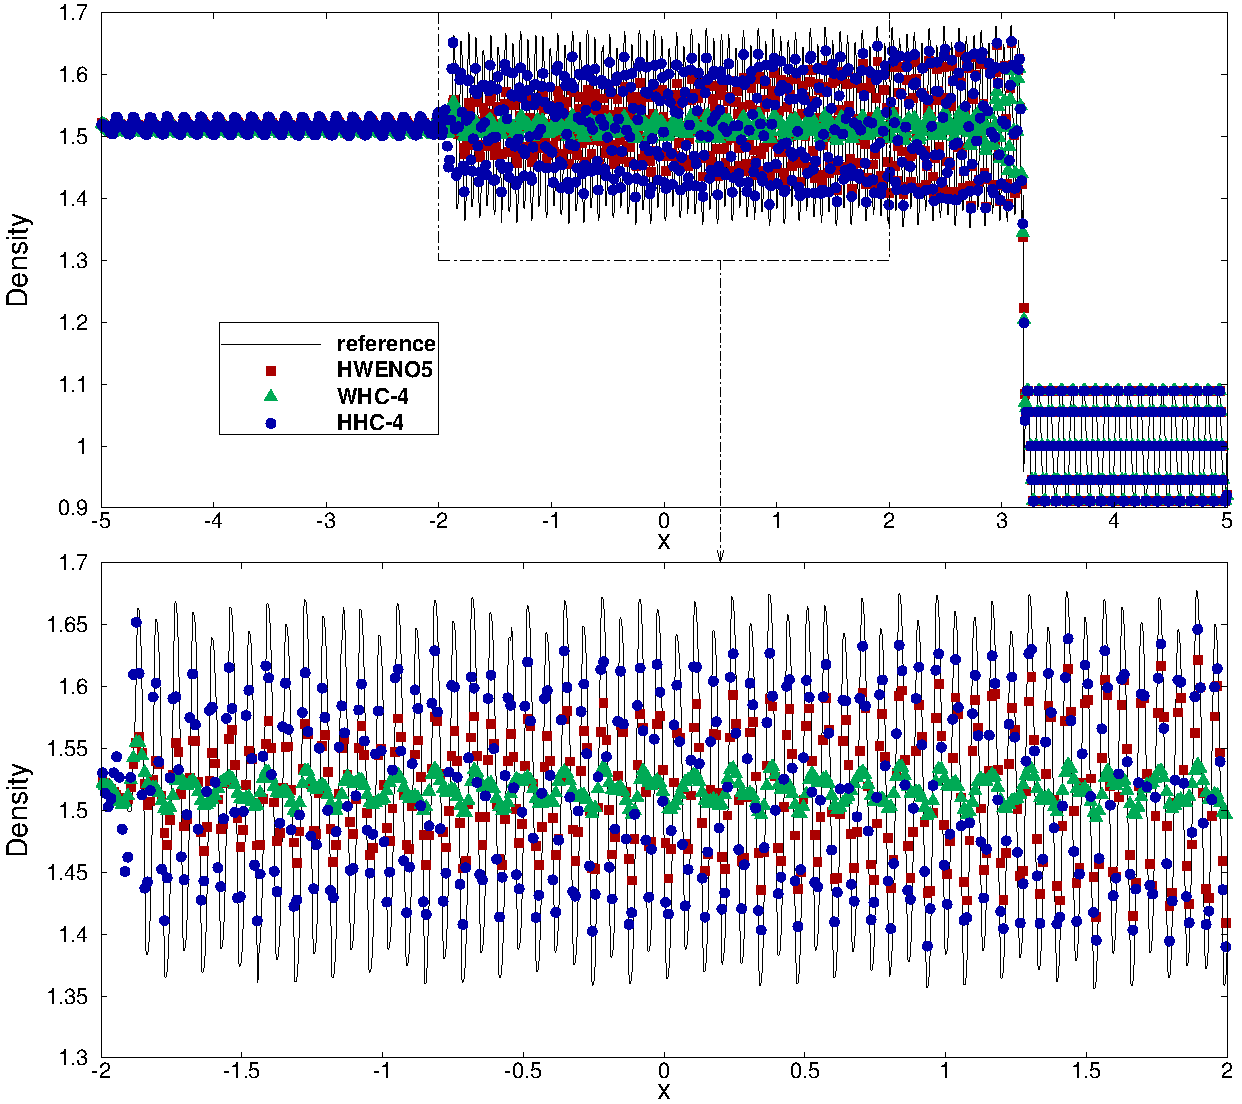
\includegraphics[height=0.33\textheight]{fig/1D/Ex4.pdf}}
%     \\
%     \subfigure[爆炸波问题]{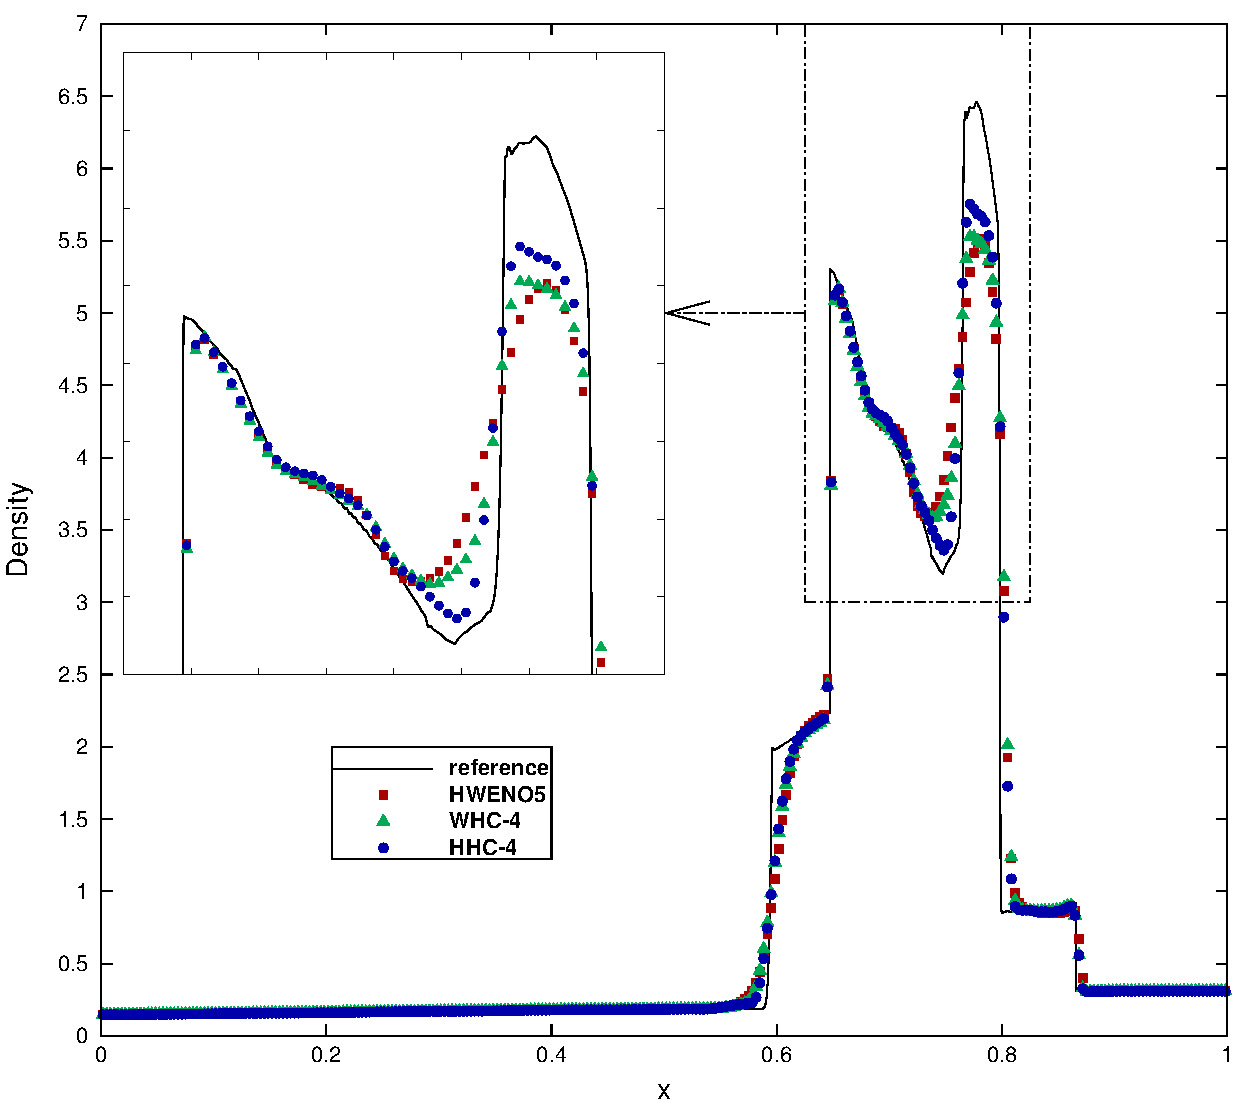
\includegraphics[height=0.33\textheight]{fig/1D/Ex5.pdf}}
%     \hspace{10mm}
%     \subfigure[大压力/密度比问题]{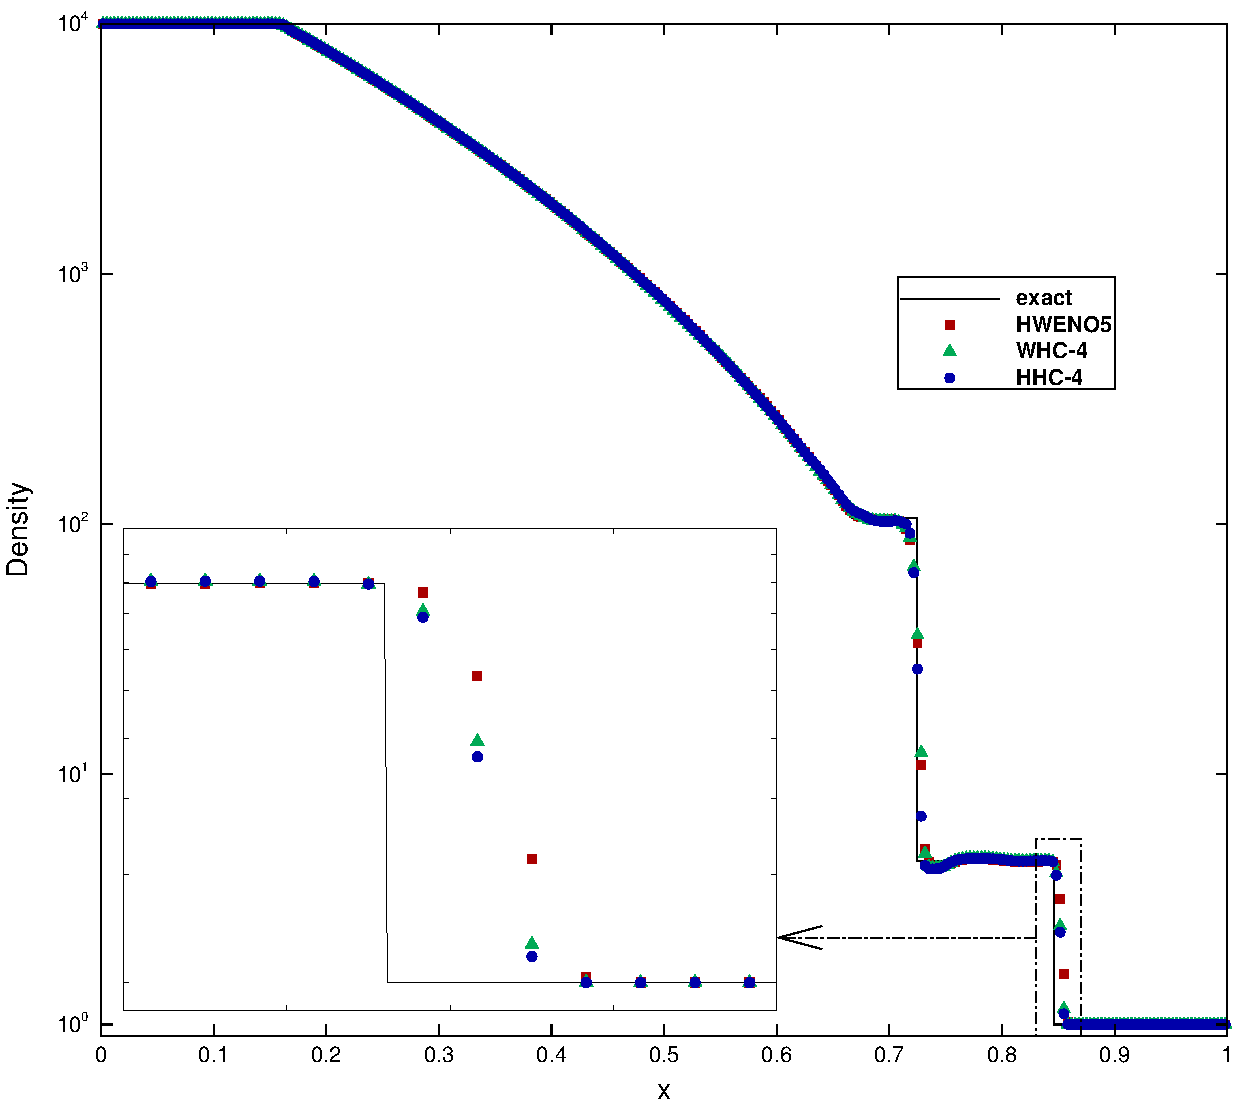
\includegraphics[height=0.33\textheight]{fig/1D/Ex6.pdf}}
%   \end{figure}

% \end{frame}

\begin{frame}{一维欧拉方程组的Lax激波管问题}
  
  \begin{example}[一维欧拉方程组的Lax激波管问题]
    \label{ex:lax}
    这是一个黎曼问题,
    以欧拉方程组作为模型,
    初值为
    \begin{equation*}
      \begin{aligned}
        (\rho,\rho u,\rho E)(x,0)=
        \begin{cases}
          (0.445,0.311,8.928), & x<0,  \\
          (0.5,0,1.4275),      & x>0.
        \end{cases}
      \end{aligned}
    \end{equation*}
  \end{example}
  
\end{frame}

\begin{frame}{一维欧拉方程组的Lax激波管问题结果}
  
  \begin{figure}[htbp]
    \centering
    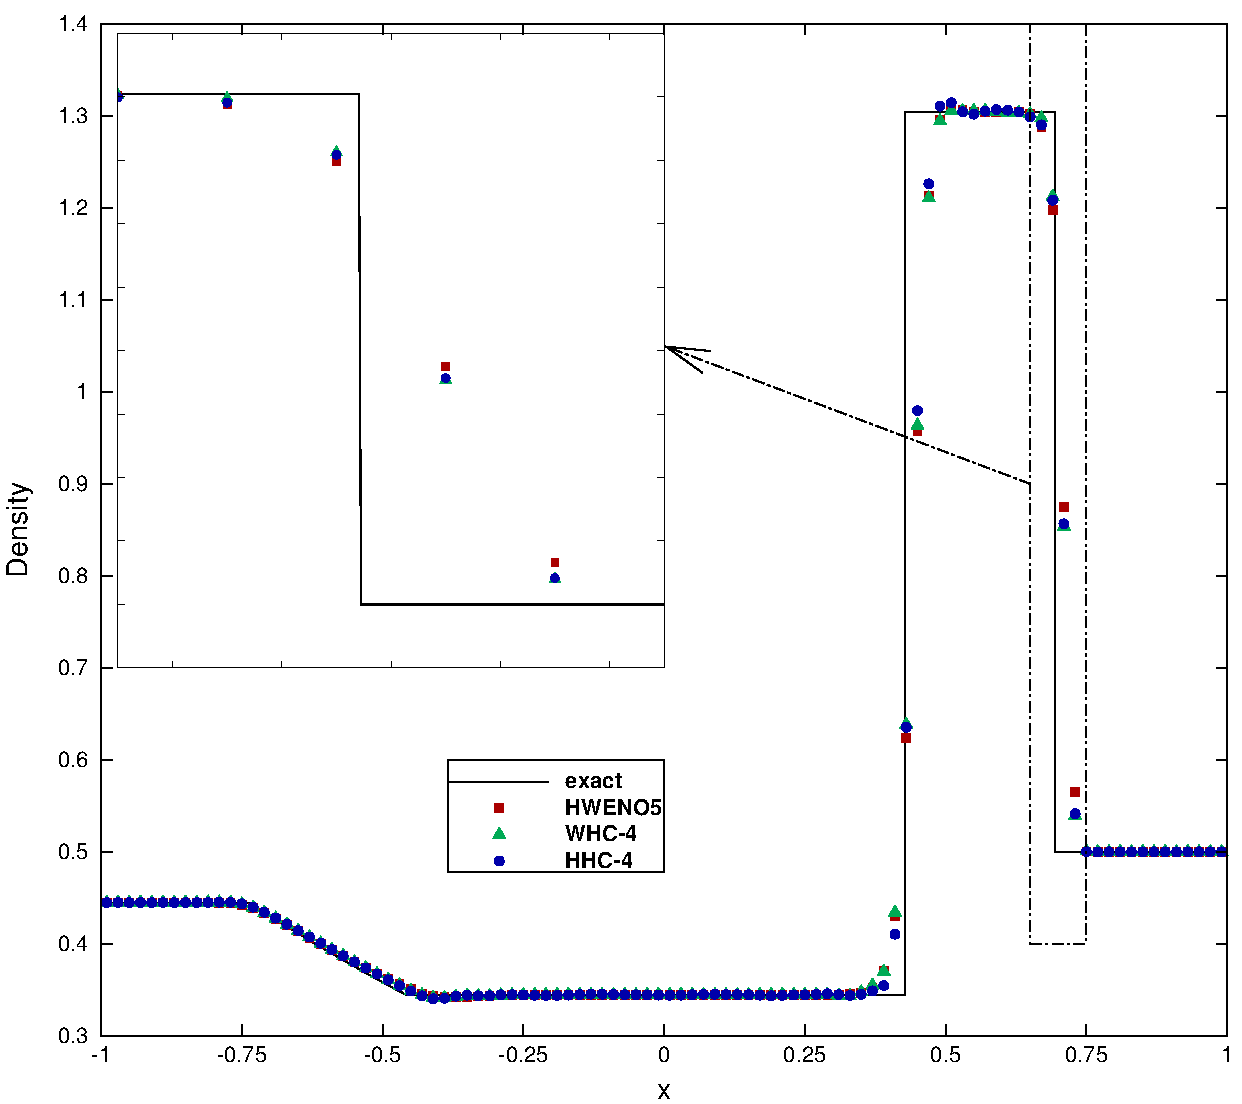
\includegraphics[height=0.75\textheight]{fig/1D/Ex2.pdf}
    \caption{一维数值格式在例 \ref{ex:lax} 中密度的图像。
      展示的是$t^{tem} = 0.28$时刻,
      $100$个网格的结果。
    }
    \label{fig:2_1}
  \end{figure}
  
\end{frame}

\begin{frame}{一维欧拉方程组的Shu-Osher问题}
  
  \begin{example}[一维欧拉方程组的Shu-Osher问题]
    \label{ex:osher}
    这个问题最初是由Shu和Osher在文献 \citep{ShuOsherProblem} 中提出的,
    以欧拉方程组作为模型,
    初值为
    \begin{equation*}
      \begin{aligned}
        (\rho,u,p)(x,0)=
        \begin{cases}
          (3.857143,2.629369,10.33333), & x<-4,  \\
          (1 + 0.2\sin(5 x),0,1),       & x>-4.
        \end{cases}
      \end{aligned}
    \end{equation*}
  \end{example}
  
\end{frame}

\begin{frame}{一维欧拉方程组的Shu-Osher问题结果}
  
  \begin{figure}[htbp]
    \centering
    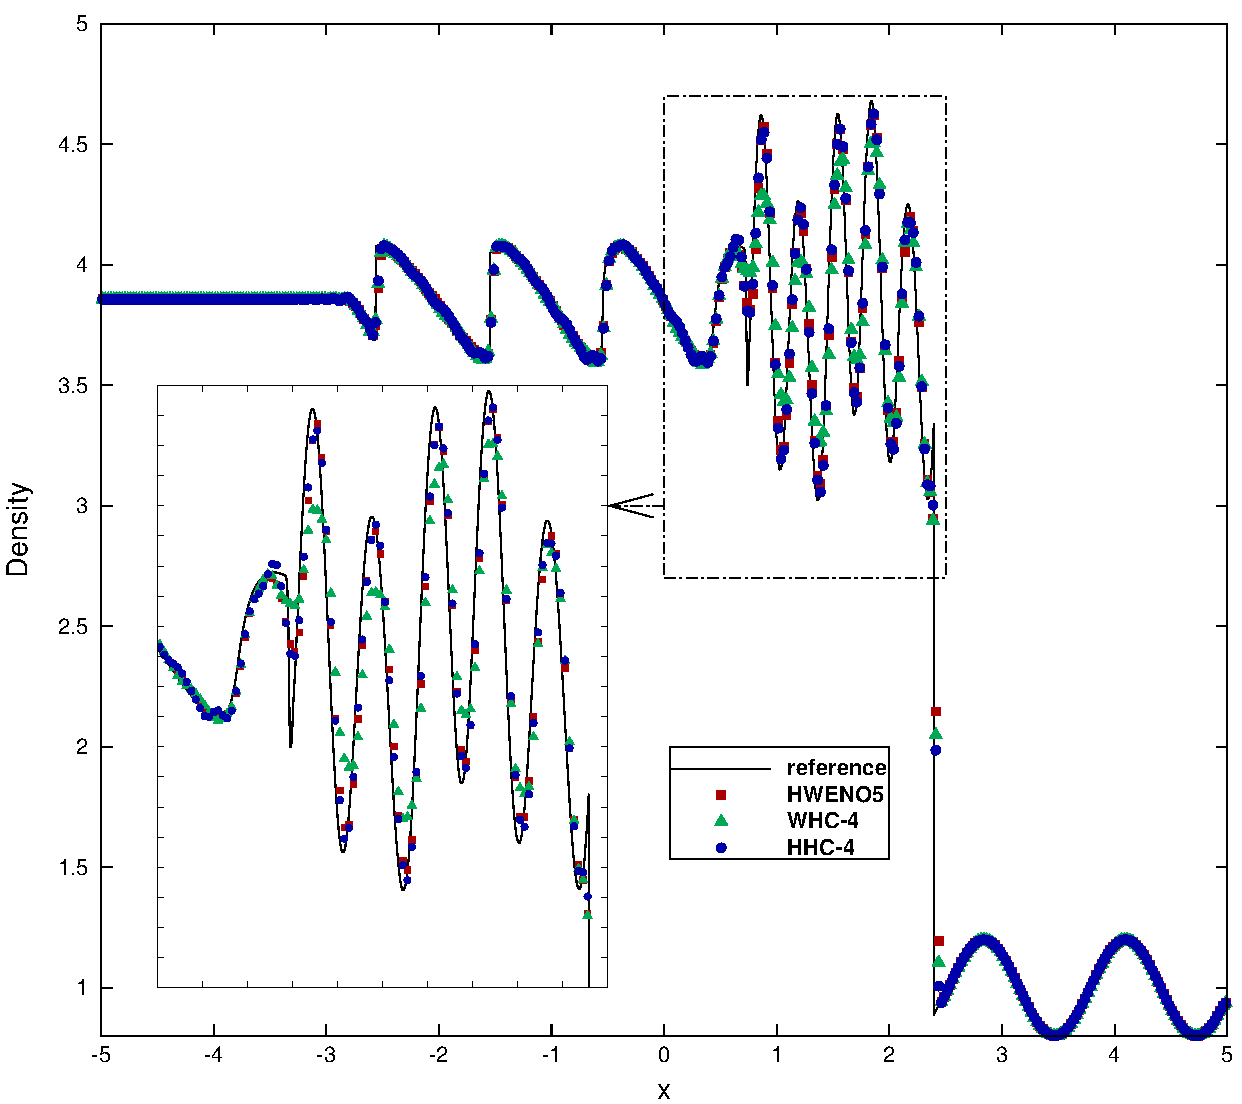
\includegraphics[height=0.75\textheight]{fig/1D/Ex3.pdf}
    \caption{一维数值格式在例 \ref{ex:osher} 中密度的图像。
      展示的是$t^{tem} = 1.8$时刻,
      $400$个网格的结果。
    }
    \label{fig:3_1}
  \end{figure}
  
\end{frame}

\begin{frame}{一维欧拉方程组的Titarev-Toro问题}
  
  \begin{example}[一维欧拉方程组的Titarev-Toro问题]
    \label{ex:toro}
    这个问题最初是由Titarev和Toro在文献 \citep{ToroProblem} 中提出的,
    以欧拉方程组作为模型,
    初值为
    \begin{equation*}
      \begin{aligned}
        (\rho, u, p)(x,0)=
        \begin{cases}
          (1.515695,0.523346,1.805),  & x<-4.5,  \\
          (1 + 0.1\sin(20\pi x),0,1), & x>-4.5.
        \end{cases}
      \end{aligned}
    \end{equation*}
  \end{example}
  
\end{frame}

\begin{frame}{一维欧拉方程组的Titarev-Toro问题结果}
  
  \begin{figure}[htbp]
    \centering
    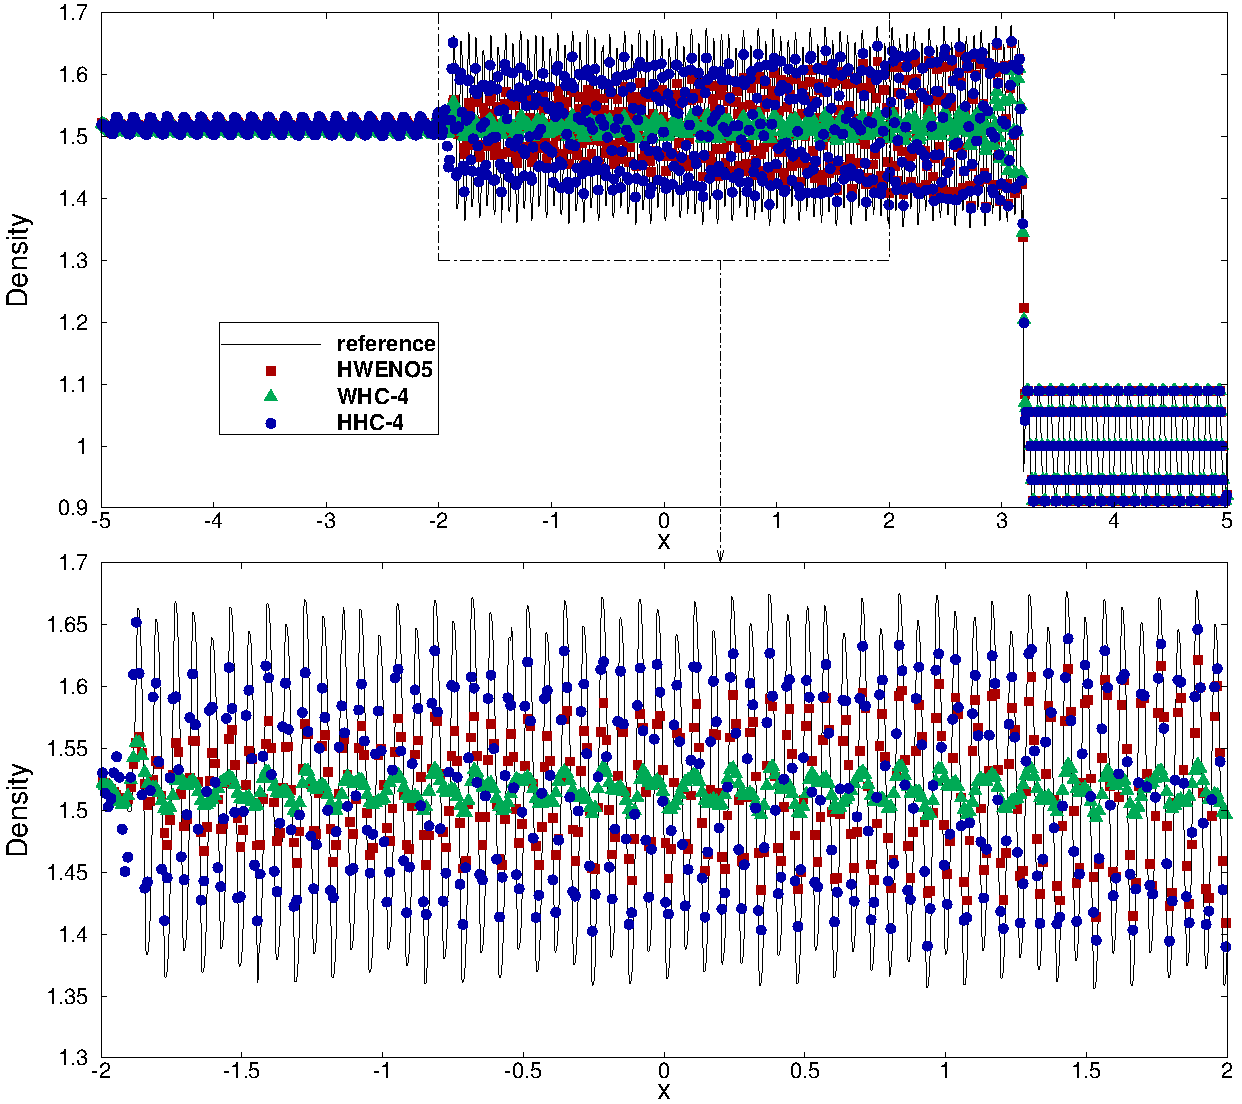
\includegraphics[height=0.75\textheight]{fig/1D/Ex4.pdf}
    \caption{一维数值格式在例 \ref{ex:toro} 中密度的图像。
      展示的是$t^{tem} = 5$时刻,
      $1000$个网格的结果。
    }
    \label{fig:4_1}
  \end{figure}
  
\end{frame}

\begin{frame}{一维欧拉方程组的爆炸波问题}
  
  \begin{example}[一维欧拉方程组的爆炸波问题]
    \label{ex:blast-wave}
    这个问题最初是由Woodward和Colella在文献 \citep{frontStep-BlastProblem} 中提出的,
    以欧拉方程组作为模型,
    初值为
    \begin{equation*}
      \begin{aligned}
        (\rho,u,p)(x,0)=
        \begin{cases}
          (1,0,10^3),    & x<0.1,     \\
          (1,0,10^{-2}), & 0.1<x<0.9, \\
          (1,0,10^2),    & x>0.9.
        \end{cases}
      \end{aligned}
    \end{equation*}
    在计算区域的两侧,
    使用了反射边界条件。
  \end{example}
  
\end{frame}

\begin{frame}{一维欧拉方程组的爆炸波问题结果}
  
  \begin{figure}[htbp]
    \centering
    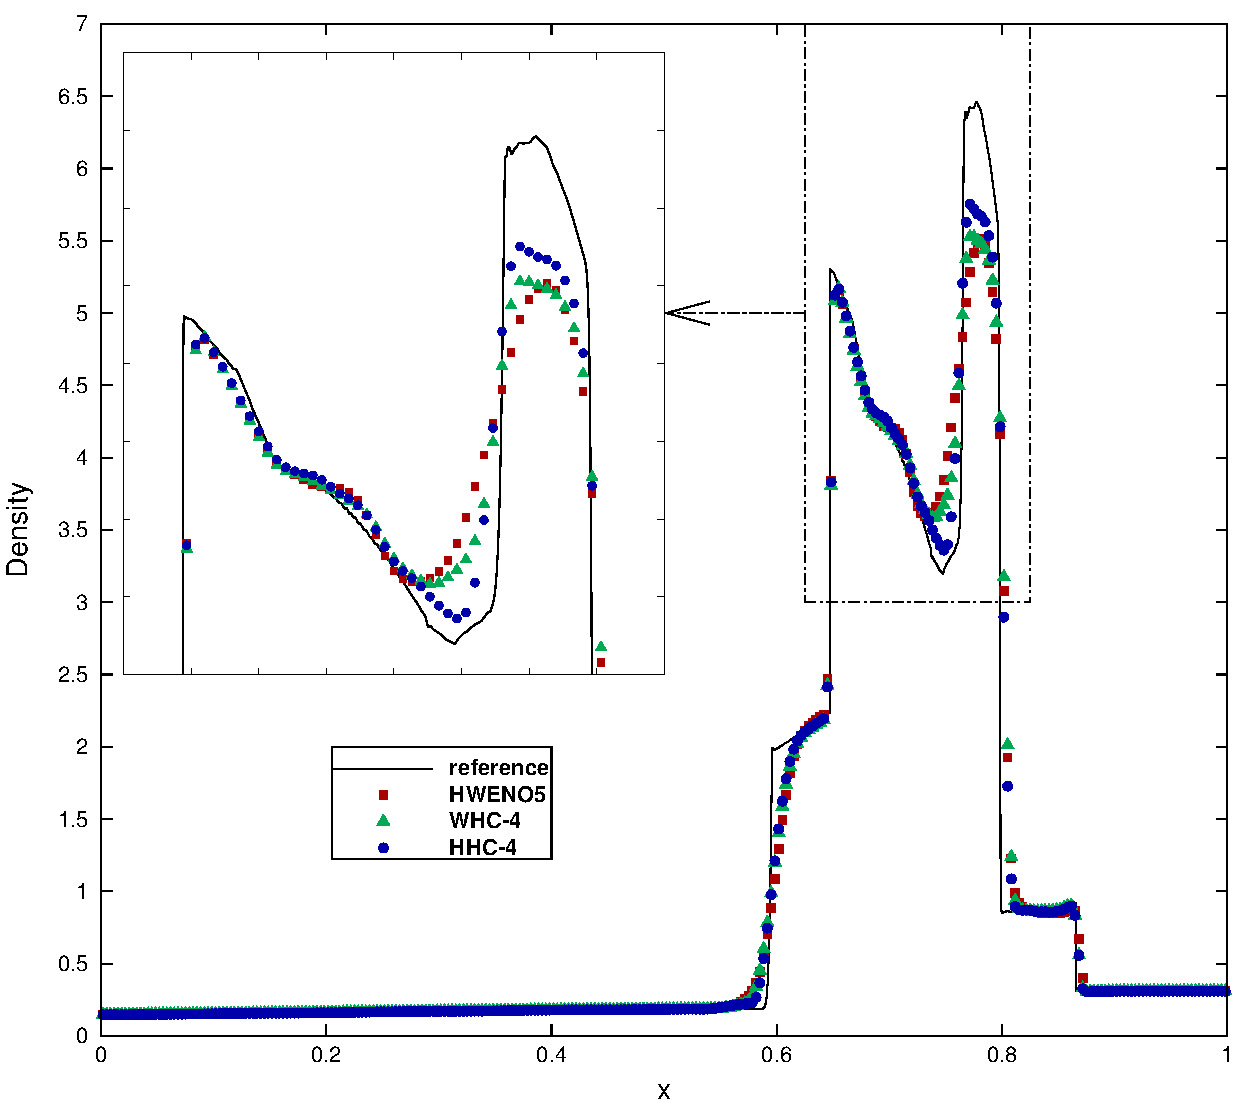
\includegraphics[height=0.75\textheight]{fig/1D/Ex5.pdf}
    \caption{一维数值格式在例 \ref{ex:blast-wave} 中密度的图像。
      展示的是$t^{tem} = 0.038$时刻,
      $300$个网格的结果。
    }
    \label{fig:5_1}
  \end{figure}
  
\end{frame}

\begin{frame}{一维欧拉方程组的大压力/密度比问题}
  
  \begin{example}[一维欧拉方程组的大压力/密度比问题]
    \label{ex:large-ratio}
    这个问题最初是由Tang和Liu在文献 \citep{LPDRP} 中提出的,
    以欧拉方程组作为模型,
    初值为
    \begin{equation*}
      \begin{aligned}
        (\rho, u, p)(x,0)=
        \begin{cases}
          (10^4,0,10^4), & x<0.3,  \\
          (1,0,1),       & x>0.3.
        \end{cases}
      \end{aligned}
    \end{equation*}
  \end{example}
  
\end{frame}

\begin{frame}{一维欧拉方程组的大压力/密度比问题结果}
  
  \begin{figure}[htbp]
    \centering
    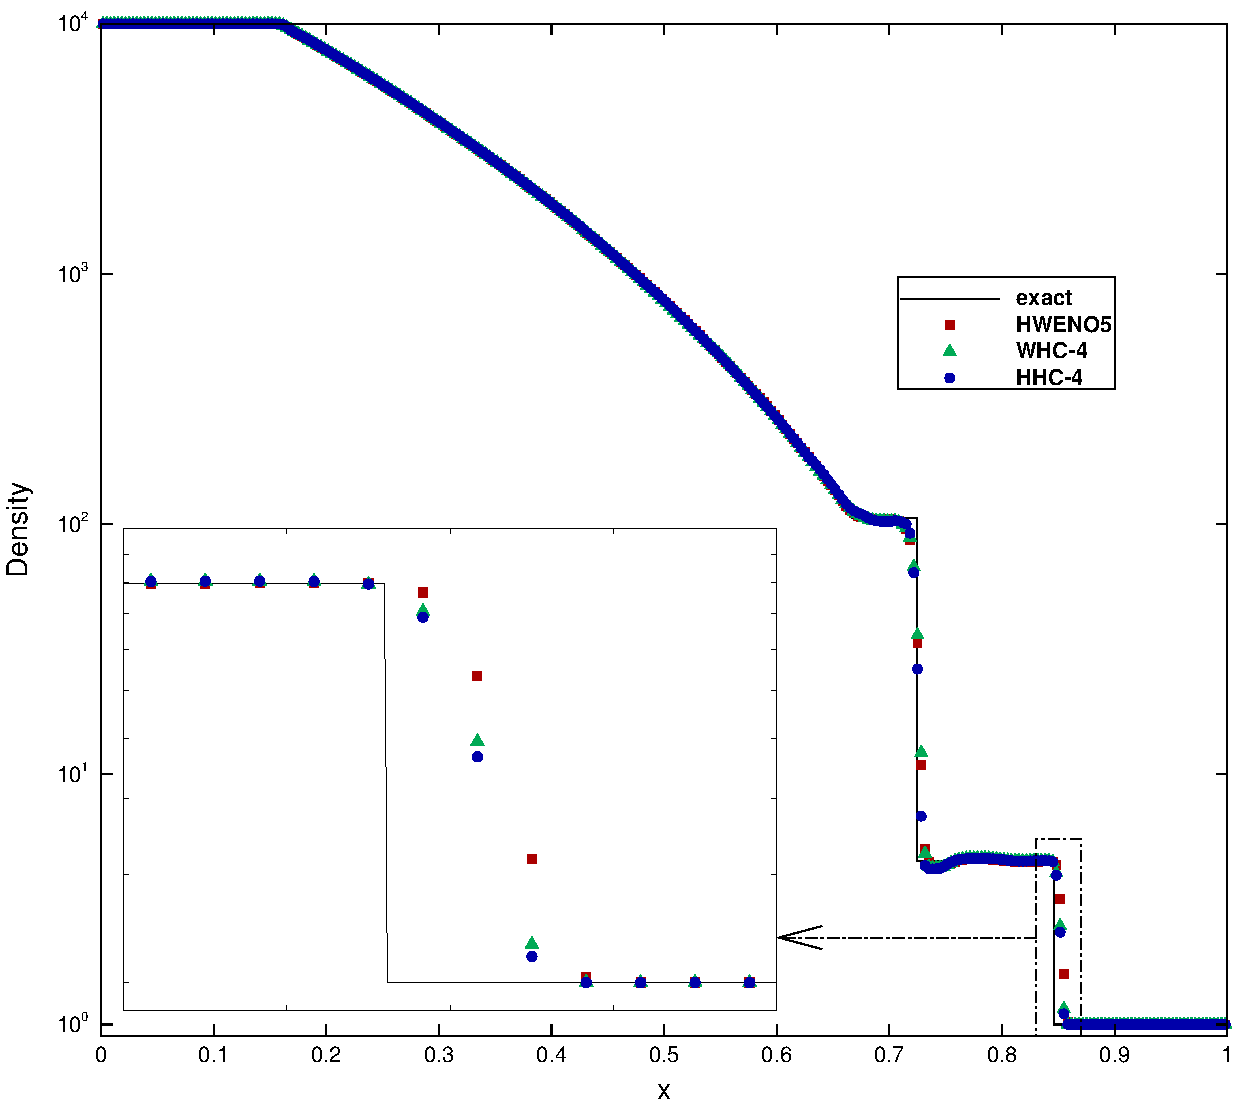
\includegraphics[height=0.75\textheight]{fig/1D/Ex6.pdf}
    \caption{一维数值格式在例 \ref{ex:large-ratio} 中密度的图像。
      展示的是$t^{tem} = 0.12$时刻,
      $300$个网格的结果。
    }
    \label{fig:6_1}
  \end{figure}
  
\end{frame}

\subsection{空间八阶精度格式及其数值实验}

\begin{frame}{WHC-8和HHC-8格式}
  
  得到空间八阶的两步四阶格式的步骤:
  
  \begin{itemize}[<+->]
    \item 用从八阶线性重构导出的多项式替换四阶线性重构导出的多项式
    \item 重新计算相应的光滑因子
    \item 调整格式中的参数(WHC-8格式中的$q=3$和HHC-8格式中的$\bar\vartheta=500000$)
  \end{itemize}
  
\end{frame}

\begin{frame}{一维欧拉方程组的线性退化的精度测试结果}
  
  \vspace{-3mm}
  \begin{columns}
    \begin{column}{0.2\textwidth}
      
      \centering
      
      WHC-8格式
      
      \vspace{0.4\textheight}
      
      HHC-8格式
      
    \end{column}
    \begin{column}{0.8\textwidth}
      \begin{tiny}
        \def\titleintable{CFL&$h$&Nstep&$L^1$-error&$L^1$-order&$L^\infty$-error&$L^\infty$-order\\}
\begin{table}[htbp]
	\caption{HC-6格式在\cref{ex:1D-acc2-re} 中密度的$L^1$和$L^\infty$误差和误差阶。展示的是$t^{tem} = 10$时刻的结果。}
	\label{ta:1D-ex2-HC6}
	\centering
	\begin{tabular}{ccccccc}
		\toprule
		\titleintable
		\midrule
		0.6   & 2/40  & 775   & 8.27459e-07 &          & 1.29667e-06 &          \\
		0.424 & 2/80  & 2190  & 1.86981e-08 & 5.46772  & 2.94233e-08 & 5.46171  \\
		\midrule
		0.6   & 2/80  & 1549  & 5.14263e-08 &          & 8.07340e-08 &          \\
		0.424 & 2/160 & 4381  & 7.21427e-07 & -3.81027 & 2.66267e-06 & -5.04355 \\
		\midrule
		0.6   & 2/160 & 3098  & 7.52045e-09 &          & 2.30543e-08 &          \\
		0.424 & 2/320 & 8761  & 2.90710e-07 & -5.27262 & 8.54718e-07 & -5.21234 \\
		\midrule
		0.6   & 2/320 & 6195  & 3.87887e-07 &          & 1.63360e-06 &          \\
		0.424 & 2/640 & 17521 & 4.45954e-07 & -0.20126 & 1.40088e-06 & 0.22173  \\
		\bottomrule
	\end{tabular}
\end{table}

\begin{table}[htbp]
	\caption{HC-8格式在\cref{ex:1D-acc2-re} 中密度的$L^1$和$L^\infty$误差和误差阶。展示的是$t^{tem} = 10$时刻的结果。}
	\label{ta:1D-ex2-HC8}
	\centering
	\begin{tabular}{ccccccc}
		\toprule
		\titleintable
		\midrule
		0.6 & 20  & 2/387   & 2.30758e-06 &         & 3.64246e-06 &         \\
		0.3 & 40  & 2/1549  & 1.00355e-08 & 7.84513 & 1.57549e-08 & 7.85297 \\
		\midrule
		0.6 & 40  & 2/775   & 8.53015e-08 &         & 1.34196e-07 &         \\
		0.3 & 80  & 2/3098  & 3.59234e-10 & 7.89150 & 5.64030e-10 & 7.89435 \\
		\midrule
		0.6 & 80  & 2/1549  & 3.87437e-09 &         & 6.07971e-09 &         \\
		0.3 & 160 & 2/6195  & 1.56789e-11 & 7.94900 & 2.47085e-11 & 7.94285 \\
		\midrule
		0.6 & 160 & 2/3098  & 2.13053e-10 &         & 3.34755e-10 &         \\
		0.3 & 320 & 2/12389 & 8.64611e-13 & 7.94495 & 1.79901e-12 & 7.53976 \\
		\bottomrule
	\end{tabular}
\end{table}

\begin{table}[htbp]
	\caption{WHC-8格式在\cref{ex:1D-acc2-re} 中密度的$L^1$和$L^\infty$误差和误差阶。展示的是$t^{tem} = 10$时刻的结果。}
	\label{ta:1D-ex2-WHC8}
	\centering
	\begin{tabular}{ccccccc}
		\toprule
		\titleintable
		\midrule
		0.6 & 20  & 2/387   & 2.30758e-06 &         & 3.64246e-06 &         \\
		0.3 & 40  & 2/1549  & 1.00355e-08 & 7.84513 & 1.57549e-08 & 7.85297 \\
		\midrule
		0.6 & 40  & 2/775   & 8.53015e-08 &         & 1.34196e-07 &         \\
		0.3 & 80  & 2/3098  & 3.59238e-10 & 7.89149 & 5.64031e-10 & 7.89435 \\
		\midrule
		0.6 & 80  & 2/1549  & 3.87437e-09 &         & 6.07972e-09 &         \\
		0.3 & 160 & 2/6195  & 1.56794e-11 & 7.94895 & 2.47098e-11 & 7.94278 \\
		\midrule
		0.6 & 160 & 2/3098  & 2.13052e-10 &         & 3.34754e-10 &         \\
		0.3 & 320 & 2/12389 & 8.67489e-13 & 7.94014 & 1.80767e-12 & 7.53283 \\
		\bottomrule
	\end{tabular}
\end{table}

\begin{table}[htbp]
	\caption{HHC-8格式在\cref{ex:1D-acc2-re} 中密度的$L^1$和$L^\infty$误差和误差阶。展示的是$t^{tem} = 10$时刻的结果。}
	\label{ta:1D-ex2-HHC8}
	\centering
	\begin{tabular}{ccccccc}
		\toprule
		\titleintable
		\midrule
		0.6 & 20  & 2/387   & 2.30758e-06 &         & 3.64246e-06 &         \\
		0.3 & 40  & 2/1549  & 1.00355e-08 & 7.84513 & 1.57549e-08 & 7.85297 \\
		\midrule
		0.6 & 40  & 2/775   & 8.53015e-08 &         & 1.34196e-07 &         \\
		0.3 & 80  & 2/3098  & 3.59237e-10 & 7.89149 & 5.64027e-10 & 7.89436 \\
		\midrule
		0.6 & 80  & 2/1549  & 3.87437e-09 &         & 6.07972e-09 &         \\
		0.3 & 160 & 2/6195  & 1.56783e-11 & 7.94905 & 2.47069e-11 & 7.94295 \\
		\midrule
		0.6 & 160 & 2/3098  & 2.13050e-10 &         & 3.34751e-10 &         \\
		0.3 & 320 & 2/12389 & 8.66274e-13 & 7.94215 & 1.80056e-12 & 7.53850 \\
		\bottomrule
	\end{tabular}
\end{table}
\undef\titleintable
      \end{tiny}
    \end{column}
  \end{columns}
  
\end{frame}

\begin{frame}{一维欧拉方程组的非线性的精度测试结果}
  
  \vspace{-3mm}
  \begin{columns}
    \begin{column}{0.2\textwidth}
      
      \centering
      
      WHC-8格式
      
      \vspace{0.4\textheight}
      
      HHC-8格式
      
    \end{column}
    \begin{column}{0.8\textwidth}
      \begin{tiny}
        \def\titleintable{CFL&$h$&Nstep&$L^1$-error&$L^1$-order&$L^\infty$-error&$L^\infty$-order\\}
% \begin{table}[htbp]
% 	\caption{HC-8格式在例 \ref{ex:1D-acc3} 中密度的$L^1$和$L^\infty$误差和误差阶。展示的是$t^{tem} = 3$时刻的结果。}
% 	\label{ta:1D-ex3-HC8}
% 	\centering
% 	\begin{tabular}{ccccccc}
% 		\toprule
% 		\titleintable
% 		\midrule
% 		0.6 & $2\pi$/80   & 77   & 1.17348e-07 &         & 2.17942e-06 &         \\
% 		0.3 & $2\pi$/160  & 306  & 9.32693e-10 & 6.97518 & 2.03143e-08 & 6.74530 \\
% 		\midrule
% 		0.6 & $2\pi$/160  & 153  & 5.21317e-09 &         & 1.04608e-07 &         \\
% 		0.3 & $2\pi$/320  & 612  & 3.36388e-11 & 7.27589 & 7.47703e-10 & 7.12831 \\
% 		\midrule
% 		0.6 & $2\pi$/320  & 306  & 2.72365e-10 &         & 4.77446e-09 &         \\
% 		0.3 & $2\pi$/640  & 1223 & 1.39036e-12 & 7.61394 & 2.82590e-11 & 7.40048 \\
% 		\midrule
% 		0.6 & $2\pi$/640  & 612  & 1.63513e-11 &         & 2.68696e-10 &         \\
% 		0.3 & $2\pi$/1280 & 2445 & 9.85380e-14 & 7.37451 & 1.33188e-12 & 7.65637 \\
% 		\bottomrule
% 	\end{tabular}
% \end{table}

\begin{table}[htbp]
	% \caption{WHC-8格式在例 \ref{ex:1D-acc3} 中密度的$L^1$和$L^\infty$误差和误差阶。展示的是$t^{tem} = 3$时刻的结果。}
	\label{ta:1D-ex3-WHC8}
	\centering
	\begin{tabular}{ccccccc}
		\toprule
		\titleintable
		\midrule
		0.6 & $2\pi$/80   & 77   & 1.17348e-07 &              & 2.17942e-06 &              \\
		0.3 & $2\pi$/160  & 306  & 9.32693e-10 & \hl{6.97518} & 2.03143e-08 & \hl{6.74530} \\
		\midrule
		0.6 & $2\pi$/160  & 153  & 5.21317e-09 &              & 1.04608e-07 &              \\
		0.3 & $2\pi$/320  & 612  & 3.36388e-11 & \hl{7.27589} & 7.47703e-10 & \hl{7.12831} \\
		\midrule
		0.6 & $2\pi$/320  & 306  & 2.72365e-10 &              & 4.77446e-09 &              \\
		0.3 & $2\pi$/640  & 1223 & 1.39030e-12 & \hl{7.61400} & 2.82586e-11 & \hl{7.40050} \\
		\midrule
		0.6 & $2\pi$/640  & 612  & 1.63512e-11 &              & 2.68696e-10 &              \\
		0.3 & $2\pi$/1280 & 2445 & 9.84114e-14 & \hl{7.37636} & 1.33077e-12 & \hl{7.65757} \\
		\bottomrule
	\end{tabular}
\end{table}

\begin{table}[htbp]
	% \caption{HHC-8格式在例 \ref{ex:1D-acc3} 中密度的$L^1$和$L^\infty$误差和误差阶。展示的是$t^{tem} = 3$时刻的结果。}
	\label{ta:1D-ex3-HHC8}
	\centering
	\begin{tabular}{ccccccc}
		\toprule
		\titleintable
		\midrule
		0.6 & $2\pi$/80   & 77   & 1.17348e-07 &              & 2.17942e-06 &              \\
		0.3 & $2\pi$/160  & 306  & 9.32693e-10 & \hl{6.97518} & 2.03143e-08 & \hl{6.74530} \\
		\midrule
		0.6 & $2\pi$/160  & 153  & 5.21317e-09 &              & 1.04608e-07 &              \\
		0.3 & $2\pi$/320  & 612  & 3.36388e-11 & \hl{7.27589} & 7.47703e-10 & \hl{7.12831} \\
		\midrule
		0.6 & $2\pi$/320  & 306  & 2.72365e-10 &              & 4.77446e-09 &              \\
		0.3 & $2\pi$/640  & 1223 & 1.39036e-12 & \hl{7.61394} & 2.82580e-11 & \hl{7.40054} \\
		\midrule
		0.6 & $2\pi$/640  & 612  & 1.63512e-11 &              & 2.68697e-10 &              \\
		0.3 & $2\pi$/1280 & 2445 & 9.84530e-14 & \hl{7.37575} & 1.33171e-12 & \hl{7.65655} \\
		\bottomrule
	\end{tabular}
\end{table}
\undef\titleintable
      \end{tiny}
    \end{column}
  \end{columns}
  
\end{frame}

\begin{frame}{数值格式的时间效率}
  
  \centering
  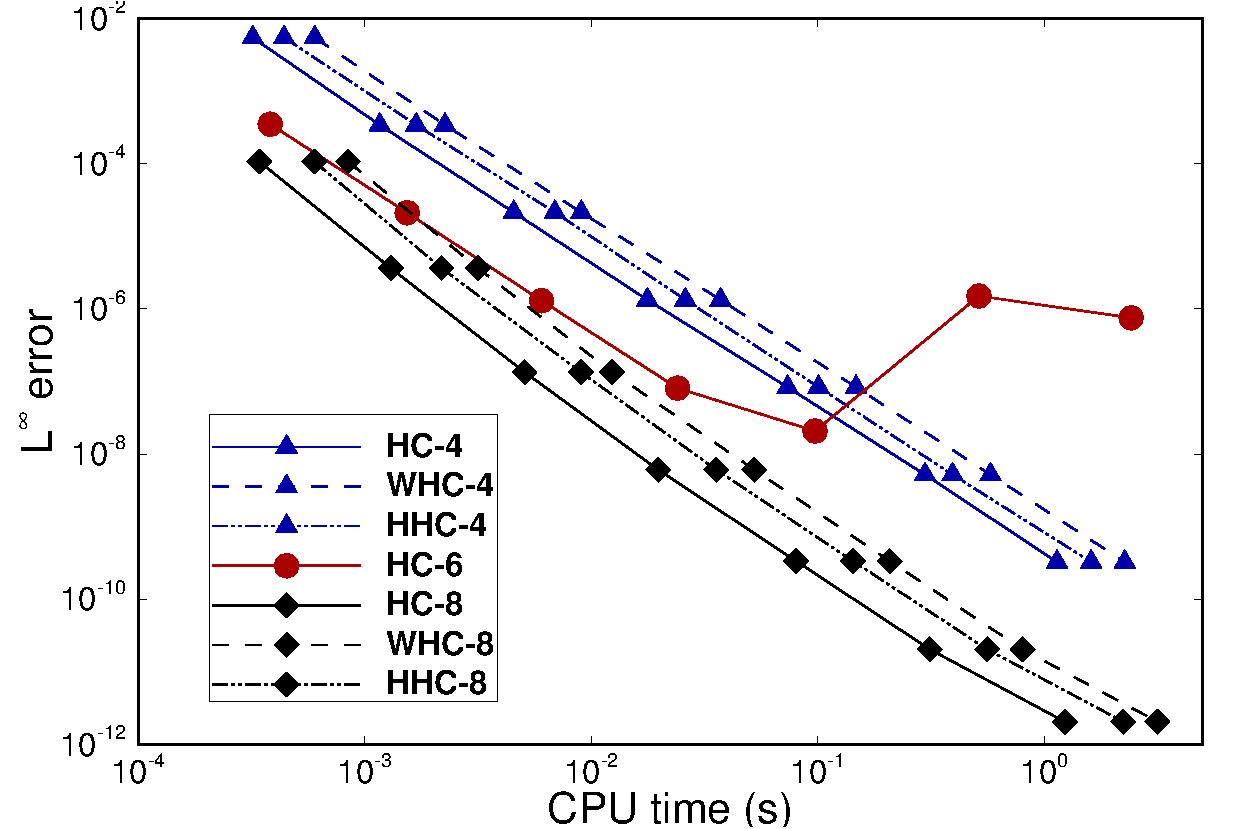
\includegraphics[height=0.85\textheight]{fig/Time/Time-1D.pdf}
  
\end{frame}

\section[二维两步四阶数值格式]{二维基于紧致Hermite重构的双曲守恒律两步四阶数值格式}

\begin{frame}{二维基于紧致Hermite重构的双曲守恒律两步四阶数值格式}
  
  \begin{itemize}[<+->]
    \item 我们想要基于二维改进的两步四阶时间推进框架,
          设计一个两步四阶数值格式。
          
    \item 解法器:
          设计了一个线性二阶LW型解法器,
          同时采用精确的Godunov解法器和GRP解法器。
          
    \item 重构:
          经过对模板的精心挑选,
          成功得到真正的二维线性紧致Hermite重构。
          
    \item 重构:
          基于二阶和四阶的线性重构,
          利用WENO和杂交选择技术,
          构造了两种四阶精度基本无振荡的非线性重构。
          
    \item 格式:
          设计了\hl{时空四阶精度基本无振荡的两步四阶格式},
          记作WHC-4和HHC-4格式。
          
    \item 格式:
          将格式推广到了空间八阶精度,
          记作WHC-8和HHC-8格式。
  \end{itemize}
  
\end{frame}

\subsection{广义黎曼问题解法器}

\begin{frame}{广义黎曼问题解法器}
  
  \begin{itemize}[<+->]
    \item Godunov解法器
          
    \item 文献 \citep{GRP_qi} 中的GRP解法器
          
          \begin{itemize}
            \item 线性声波近似的 (acoustic) GRP 解法器
                  
            \item 二维弱耦合的非线性GRP解法器
          \end{itemize}
          
    \item 新设计的线性二阶LW型解法器
  \end{itemize}
  
\end{frame}

\subsection{线性紧致Hermite重构及其相应的两步四阶格式}

\begin{frame}{二维线性紧致Hermite重构的要求}
  
  \TextAndFig[0.7\textwidth]{
    \begin{itemize}[<+->]
      \item 满足精度要求
            \begin{align*}
              {\partial_{x}^{d_1}}{\partial_{y}^{d_2}}p_{ij}(x,y) 
              = {\partial_{x}^{d_1}}{\partial_{y}^{d_2}}u(x,y)
              +{\mathcal{O}}(h^{2k-d_1-d_2}), & 
              \\
              0 \le d_1+d_2 \le 2k-1.         & 
            \end{align*}
            
      \item 二维重构在一维问题中可以退化到之前的一维重构。
            
      \item $k^2$个单元中总共有$3k^2$个自由度。
            而在$\mathcal{P}^{2k-1}$空间中,
            只需要$2k^2+k$个自由度。
            为了避免最小二乘法的计算开销,
            将会忽略其中$k^2-k$个自由度。
      \item 需要使最终的模板尽可能对称。
      \item 要确保目标单元$I_{ij}$本身在模板中。
    \end{itemize}
  }{
    \begin{figure}[htbp]
      \centering
      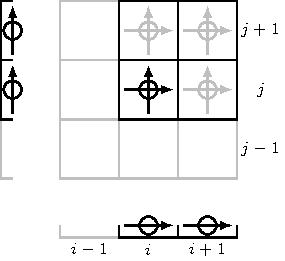
\includegraphics[width=\textwidth]{fig/tikz/case2forslides.pdf}
      \caption{单元平均值$\bar u_{ij}$由一个圆圈表示,
        而导数平均值$\bar v_{ij}$由一个向右的箭头表示,
        $\bar w_{ij}$由一个向左的箭头表示。}
    \end{figure}
  }
  
\end{frame}

\begin{frame}{二维线性紧致Hermite重构}
  
  \begin{figure}[htbp]
    \centering
    \subfigure[$k=1$的情形。]{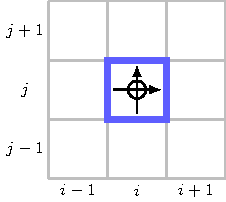
\includegraphics[width=0.24\textwidth]{fig/tikz/case1.pdf}}
    \subfigure[$k=2$的第一种情形。]{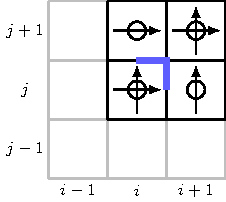
\includegraphics[width=0.24\textwidth]{fig/tikz/case2.pdf}}
    \subfigure[$k=2$第二种的情形。]{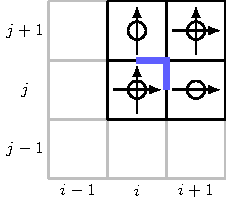
\includegraphics[width=0.24\textwidth]{fig/tikz/case2-2.pdf}}
    \subfigure[将图~(b)旋转得到的情形。]{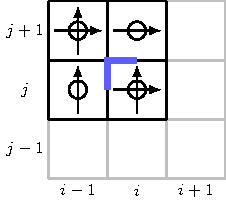
\includegraphics[width=0.24\textwidth]{fig/tikz/case2-ratation.pdf}}
    \caption{当$k=1,2$时的模板示意图。
      从此模板得到的重构多项式所应用的范围是蓝线所标识的。
    }
  \end{figure}
  
  \onslide<2>
  \colorBOX[yellow!40]{\textwidth}{0mm}{0mm}{
    使用改进的两步四阶时间推进框架,
    其中重构采用二维线性紧致Hermite重构,
    解法器采用GRP解法器,
    就得到了相应的两步四阶格式。  
  }
  
\end{frame}

\begin{frame}{二维线性紧致Hermite重构}
  
  \FigAndTex[\textheight]{
    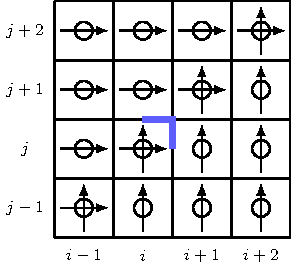
\includegraphics[height=0.8\textheight]{fig/tikz/case4.pdf}
  }{
    当$k=4$时的模板示意图。
    从此模板得到的重构多项式所应用的范围是蓝线所标识的。
  }
  
\end{frame}

\subsection[非线性紧致Hermite重构及其相应的两步四阶格式]{基本无振荡的紧致Hermite重构及其相应的两步四阶格式}

\begin{frame}{基本无振荡的紧致Hermite重构及其相应的两步四阶格式}
  
  类似一维,我们有加权型紧致Hermite重构(WHC-4重构)
  \colorBOX{12cm}{-5mm}{-6mm}{
    \begin{align*}
      u_{(i+\frac{1}{2},-), j+G}^{\text{WHC-4}}= \frac{\omega_{{f}}}{\gamma_{{f}}}u_{(i+\frac{1}{2},-), j+G}^{{f}}+ \left(1-\frac{\omega_{{f}}}{\gamma_{{f}}}\right)u_{(i+\frac{1}{2},-), j+G}^{{s}},
    \end{align*}
  }
  
  \pause
  以及杂交选择型紧致Hermite重构(HHC-4重构)
  \colorBOX{12cm}{-2mm}{-5mm}{
    \begin{equation*}
      \begin{aligned}
        u_{(i+\frac{1}{2},-), j+G}^{\text{HHC-4}}=
        \begin{cases}
          u_{(i+\frac{1}{2},-), j+G}^{{f}}, & \beta_{{f}}+\varepsilon < \bar{\vartheta}(\beta_{{s}}+\varepsilon),   \\
          u_{(i+\frac{1}{2},-), j+G}^{{s}}, & \beta_{{f}}+\varepsilon \ge\bar{\vartheta}(\beta_{{s}}+\varepsilon),
        \end{cases}
        \quad\quad
        \bar{\vartheta} = 20.
      \end{aligned}
    \end{equation*}
  }
  
  \pause
  使用改进的两步四阶时间推进框架,
  其中重构采用上述二维紧致Hermite重构,
  解法器采用GRP解法器,
  就得到了相应的两步四阶格式。
  
\end{frame}

\begin{frame}{WHC-4和HHC-4格式的紧致性}
  
  \begin{figure}[htbp]
    \centering
    \subfigure[]{\label{subfig:four-cells}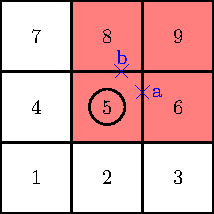
\includegraphics{fig/tikz/compact-flux.pdf}}
    \subfigure[]{\label{subfig:compact-HC4}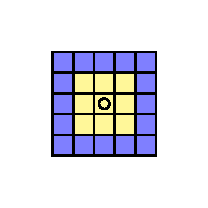
\includegraphics{fig/tikz/compact-HC4.pdf}}
    \subfigure[]{\label{subfig:compact-S2O4-HWENO5}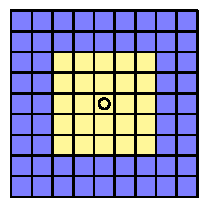
\includegraphics{fig/tikz/compact-S2O4-HWENO5.pdf}}
    \subfigure[]{\label{subfig:compact-S2O4-HWENO4}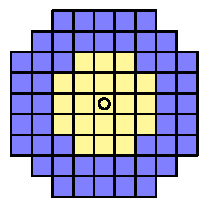
\includegraphics{fig/tikz/compact-S2O4-HWENO4.pdf}}
    \caption{
      依赖区域的示意图。
      (a) WHC-4和HHC-4格式的数值通量的依赖区域。
      (b) WHC-4和HHC-4格式的依赖区域。
      (c) 文献 \citep{du2018hermite} 中的S2O4-HWENO5格式的依赖区域。
      (d) 文献 \citep{Qiu-Shu-2005} 中的S2O4-HWENO4格式的依赖区域。
    }
  \end{figure}
  
\end{frame}

\subsection{数值实验}

\begin{frame}{二维欧拉方程组的线性退化的精度测试}
  
  \begin{example}[二维欧拉方程组的线性退化的精度测试]
    \label{ex:2D-acc2}
    这个算例选择欧拉方程组
    \begin{equation*}
      \label{eq:2D-Euler}
      \left\{
      \begin{aligned}
         & {\partial_{t}}{\bm{u}}+{\partial_{x}}{\bm{f}}({\bm{u}})+{\partial_{y}}{\bm{g}}({\bm{u}})=0, \\
         & {\bm{u}}=(\rho, \rho u, \rho v, \rho E)^\top,                                               \\
         & {\bm{f}}=(\rho u, \rho u^2+p, \rho uv, u (\rho E+p))^\top,                                  \\
         & {\bm{g}}=(\rho v, \rho uv, \rho v^2+p, v (\rho E+p))^\top,
      \end{aligned}
      \right.
    \end{equation*}
    作为模型,
    其中多方指数$\gamma$取$1.4$,
    初值为
    \begin{equation*}
      \rho(x,y,0) = 1 + 0.2\sin(\pi(x+y)), \quad u(x,y,0)=0.7, \quad v(x,y,0)=0.3, \quad p(x,y,0)=1.
    \end{equation*}
    计算区域是$[-1,1]\times[-1,1]$,
    采取周期边界条件。
    这个问题是线性退化的,
    它的精确解是${\bm{u}}(x,y,t) = {\bm{u}}(x-0.7t,y-0.3t,0)$。
  \end{example}
  
\end{frame}

\begin{frame}{二维欧拉方程组的线性退化的精度测试结果}
  
  \vspace{-3mm}
  \begin{columns}
    \begin{column}{0.2\textwidth}
      
      \centering
      
      WHC-4格式
      
      \vspace{0.4\textheight}
      
      HHC-4格式
      
    \end{column}
    \begin{column}{0.8\textwidth}
      \begin{small}
        \def\titleintable{CFL&$h$&Nstep&$L^1$-error&$L^1$-order&$L^\infty$-error&$L^\infty$-order\\}
% \begin{table}[htbp]
%   \caption{HC-4格式在例 \ref{ex:1D-acc2} 中密度的$L^1$和$L^\infty$误差和误差阶。展示的是$t^{tem} = 10$时刻的结果。}
%   \label{ta:1D-ex2-HC4}
%   \centering
%   \begin{tabular}{ccccccc}
%     \toprule
%     \titleintable
%     \midrule
%     0.6 & 2/40   & 775   & 1.35453e-05 &         & 2.12772e-05 &         \\
%     0.6 & 2/80   & 1549  & 8.46534e-07 & 4.00009 & 1.32973e-06 & 4.00010 \\
%     0.6 & 2/160  & 3098  & 5.29071e-08 & 4.00003 & 8.31064e-08 & 4.00003 \\
%     0.6 & 2/320  & 6195  & 3.30668e-09 & 4.00001 & 5.19407e-09 & 4.00002 \\
%     0.6 & 2/640  & 12389 & 2.06655e-10 & 4.00008 & 3.25390e-10 & 3.99663 \\
%     0.6 & 2/1280 & 24778 & 1.29157e-11 & 4.00003 & 2.19097e-11 & 3.89253 \\
%     \bottomrule
%   \end{tabular}
% \end{table}

\begin{table}[htbp]
  % \caption{WHC-4格式在例 \ref{ex:1D-acc2} 中密度的$L^1$和$L^\infty$误差和误差阶。展示的是$t^{tem} = 10$时刻的结果。}
  \label{ta:1D-ex2-WHC4}
  \centering
  \begin{tabular}{ccccccc}
    \toprule
    \titleintable
    \midrule
    0.6 & 2/40   & 775   & 1.35453e-05 &              & 2.12772e-05 &              \\
    0.6 & 2/80   & 1549  & 8.46533e-07 & \hl{4.00009} & 1.32973e-06 & \hl{4.00010} \\
    0.6 & 2/160  & 3098  & 5.29071e-08 & \hl{4.00003} & 8.31064e-08 & \hl{4.00003} \\
    0.6 & 2/320  & 6195  & 3.30668e-09 & \hl{4.00001} & 5.19407e-09 & \hl{4.00002} \\
    0.6 & 2/640  & 12389 & 2.06656e-10 & \hl{4.00008} & 3.25396e-10 & \hl{3.99660} \\
    0.6 & 2/1280 & 24778 & 1.29151e-11 & \hl{4.00010} & 2.18940e-11 & \hl{3.89359} \\
    \bottomrule
  \end{tabular}
\end{table}

\begin{table}[htbp]
  % \caption{HHC-4格式在例 \ref{ex:1D-acc2} 中密度的$L^1$和$L^\infty$误差和误差阶。展示的是$t^{tem} = 10$时刻的结果。}
  \label{ta:1D-ex2-HHC4}
  \centering
  \begin{tabular}{ccccccc}
    \toprule
    \titleintable
    \midrule
    0.6 & 2/40   & 775   & 1.35453e-05 &              & 2.12772e-05 &              \\
    0.6 & 2/80   & 1549  & 8.46534e-07 & \hl{4.00009} & 1.32973e-06 & \hl{4.00010} \\
    0.6 & 2/160  & 3098  & 5.29071e-08 & \hl{4.00003} & 8.31064e-08 & \hl{4.00003} \\
    0.6 & 2/320  & 6195  & 3.30668e-09 & \hl{4.00001} & 5.19407e-09 & \hl{4.00002} \\
    0.6 & 2/640  & 12389 & 2.06659e-10 & \hl{4.00008} & 3.25382e-10 & \hl{3.99669} \\
    0.6 & 2/1280 & 24778 & 1.29121e-11 & \hl{4.00043} & 2.19050e-11 & \hl{3.89280} \\
    \bottomrule
  \end{tabular}
\end{table}
\undef\titleintable
      \end{small}
    \end{column}
  \end{columns}
  
\end{frame}

\begin{frame}{二维欧拉方程组的非线性的精度测试}
  
  \begin{example}[二维欧拉方程组的非线性的精度测试]
    \label{ex:2D-acc3}
    这是一个源自文献 \citep{Gamma3-HWENO} 的数值算例,
    初始条件设定为
    \begin{align*}
       & \rho(x, y, 0)=\frac{1+0.2\sin(0.5(x+y)) }{\sqrt{6}},        \\
       & u(x, y, 0)=v(x, y, 0)=\sqrt{\frac{\gamma}{2}}\rho(x, y, 0), \\
       & p(x, y, 0)=\rho(x, y, 0)^\gamma.
    \end{align*}
    计算区域是$[0, 4\pi]\times[0, 4\pi]$,
    并且使用与例 \ref{ex:2D-acc2} 相同的
    欧拉方程组、均匀网格和周期边界。
    不过,
    多方指数$\gamma$设定为3。
  \end{example}
  
\end{frame}

\begin{frame}{二维欧拉方程组的非线性的精度测试结果}
  
  \vspace{-3mm}
  \begin{columns}
    \begin{column}{0.2\textwidth}
      
      \centering
      
      WHC-4格式
      
      \vspace{0.4\textheight}
      
      HHC-4格式
      
    \end{column}
    \begin{column}{0.8\textwidth}
      \begin{small}
        \def\titleintable{CFL&$h$&Nstep&$L^1$-error&$L^1$-order&$L^\infty$-error&$L^\infty$-order\\}
\begin{table}[htbp]
  \caption{HC-4格式在\cref{ex:2D-acc3} 中$u$的$L^1$和$L^\infty$误差和误差阶。展示的是$t^{tem} = 1$时刻的结果。}
  \label{ta:2D-ex3-HC4}
  \centering
  \begin{tabular}{ccccccc}
    \toprule
    \titleintable
    \midrule
    % 0.6 &$4\pi$/100 & 32 & 1.03900e-07 & & 4.49257e-07 & \\
    % 0.6 &$4\pi$/150 & 48 & 2.10901e-08 & 3.93283 & 1.11949e-07 & 3.42706 \\
    0.6 & $4\pi$/150 & 48  & 2.10901e-08 &         & 1.11949e-07 &         \\
    0.6 & $4\pi$/200 & 64  & 6.84370e-09 & 3.91221 & 3.00975e-08 & 4.56615 \\
    0.6 & $4\pi$/250 & 80  & 2.80492e-09 & 3.99723 & 1.23554e-08 & 3.99003 \\
    0.6 & $4\pi$/300 & 96  & 1.35184e-09 & 4.00341 & 5.97173e-09 & 3.98776 \\
    0.6 & $4\pi$/350 & 112 & 7.29333e-10 & 4.00316 & 3.23427e-09 & 3.97815 \\
    0.6 & $4\pi$/400 & 128 & 4.27356e-10 & 4.00290 & 1.91305e-09 & 3.93243 \\
    \bottomrule
  \end{tabular}
\end{table}

\begin{table}[htbp]
  \caption{WHC-4格式在\cref{ex:2D-acc3} 中$u$的$L^1$和$L^\infty$误差和误差阶。展示的是$t^{tem} = 1$时刻的结果。}
  \label{ta:2D-ex3-WHC4}
  \centering
  \begin{tabular}{ccccccc}
    \toprule
    \titleintable
    \midrule
    % 0.6 &$4\pi$/100 & 32 & 1.03900e-07 & & 4.49257e-07 & \\
    % 0.6 &$4\pi$/150 & 48 & 2.10901e-08 & 3.93283 & 1.11949e-07 & 3.42706 \\
    0.6 & $4\pi$/150 & 48  & 2.10901e-08 &         & 1.11949e-07 &         \\
    0.6 & $4\pi$/200 & 64  & 6.84370e-09 & 3.91221 & 3.00975e-08 & 4.56615 \\
    0.6 & $4\pi$/250 & 80  & 2.80492e-09 & 3.99723 & 1.23554e-08 & 3.99003 \\
    0.6 & $4\pi$/300 & 96  & 1.35184e-09 & 4.00341 & 5.97173e-09 & 3.98776 \\
    0.6 & $4\pi$/350 & 112 & 7.29333e-10 & 4.00316 & 3.23427e-09 & 3.97815 \\
    0.6 & $4\pi$/400 & 128 & 4.27356e-10 & 4.00290 & 1.91305e-09 & 3.93243 \\
    \bottomrule
  \end{tabular}
\end{table}

\begin{table}[htbp]
  \caption{HHC-4格式在\cref{ex:2D-acc3} 中$u$的$L^1$和$L^\infty$误差和误差阶。展示的是$t^{tem} = 1$时刻的结果。}
  \label{ta:2D-ex3-HHC4}
  \centering
  \begin{tabular}{ccccccc}
    \toprule
    \titleintable
    \midrule
    % 0.6 &$4\pi$/100 & 32 & 1.03900e-07 & & 4.49257e-07 & \\
    % 0.6 &$4\pi$/150 & 48 & 2.10901e-08 & 3.93283 & 1.11949e-07 & 3.42706 \\
    0.6 & $4\pi$/150 & 48  & 2.10901e-08 &         & 1.11949e-07 &         \\
    0.6 & $4\pi$/200 & 64  & 6.84370e-09 & 3.91221 & 3.00975e-08 & 4.56615 \\
    0.6 & $4\pi$/250 & 80  & 2.80492e-09 & 3.99723 & 1.23554e-08 & 3.99003 \\
    0.6 & $4\pi$/300 & 96  & 1.35184e-09 & 4.00341 & 5.97173e-09 & 3.98776 \\
    0.6 & $4\pi$/350 & 112 & 7.29333e-10 & 4.00316 & 3.23427e-09 & 3.97815 \\
    0.6 & $4\pi$/400 & 128 & 4.27356e-10 & 4.00290 & 1.91305e-09 & 3.93243 \\
    \bottomrule
  \end{tabular}
\end{table}
\undef\titleintable
      \end{small}
    \end{column}
  \end{columns}
  
\end{frame}

% \begin{frame}{二维欧拉方程组的含间断问题:黎曼问题($400 \times 400$个网格)}

%   \vspace{-4mm}
%   \begin{figure}[htbp]
%     \centering

%     \begin{multicols}{4}
%       \begin{minipage}{0.25\textwidth}
%         \vspace{0.13\textheight}
%         \centerline{WHC-4格式}
%       \end{minipage}
%       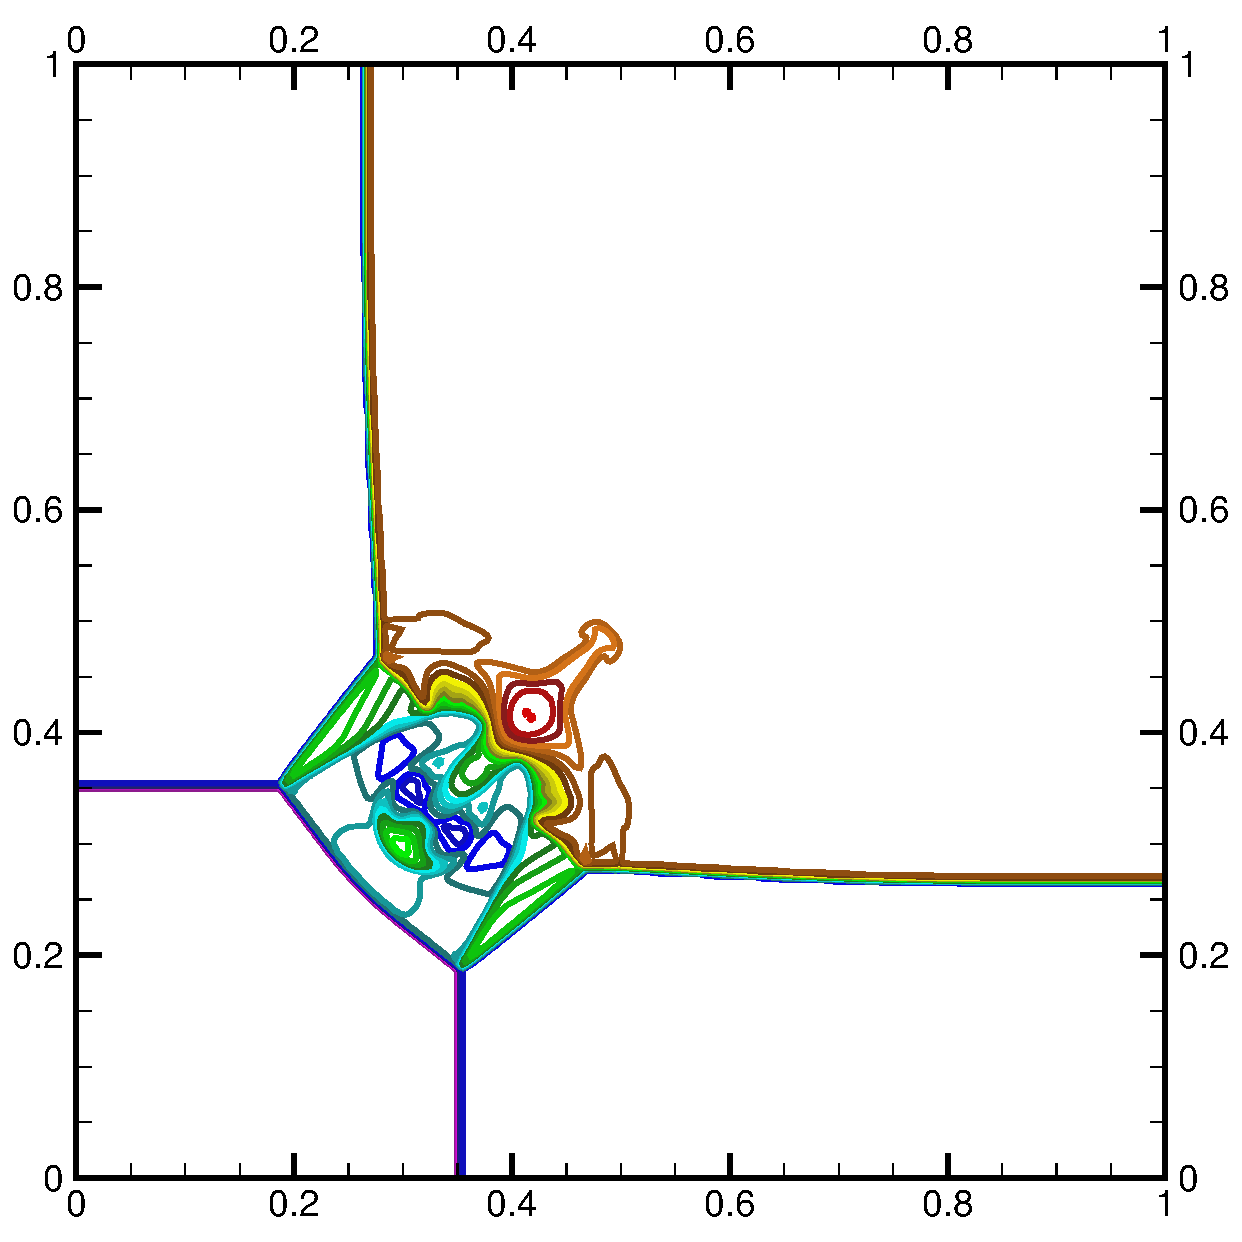
\includegraphics[height=0.4\textheight]{fig/2D/RP1_S2O4-WHC4_CFL0.600000.pdf}
%       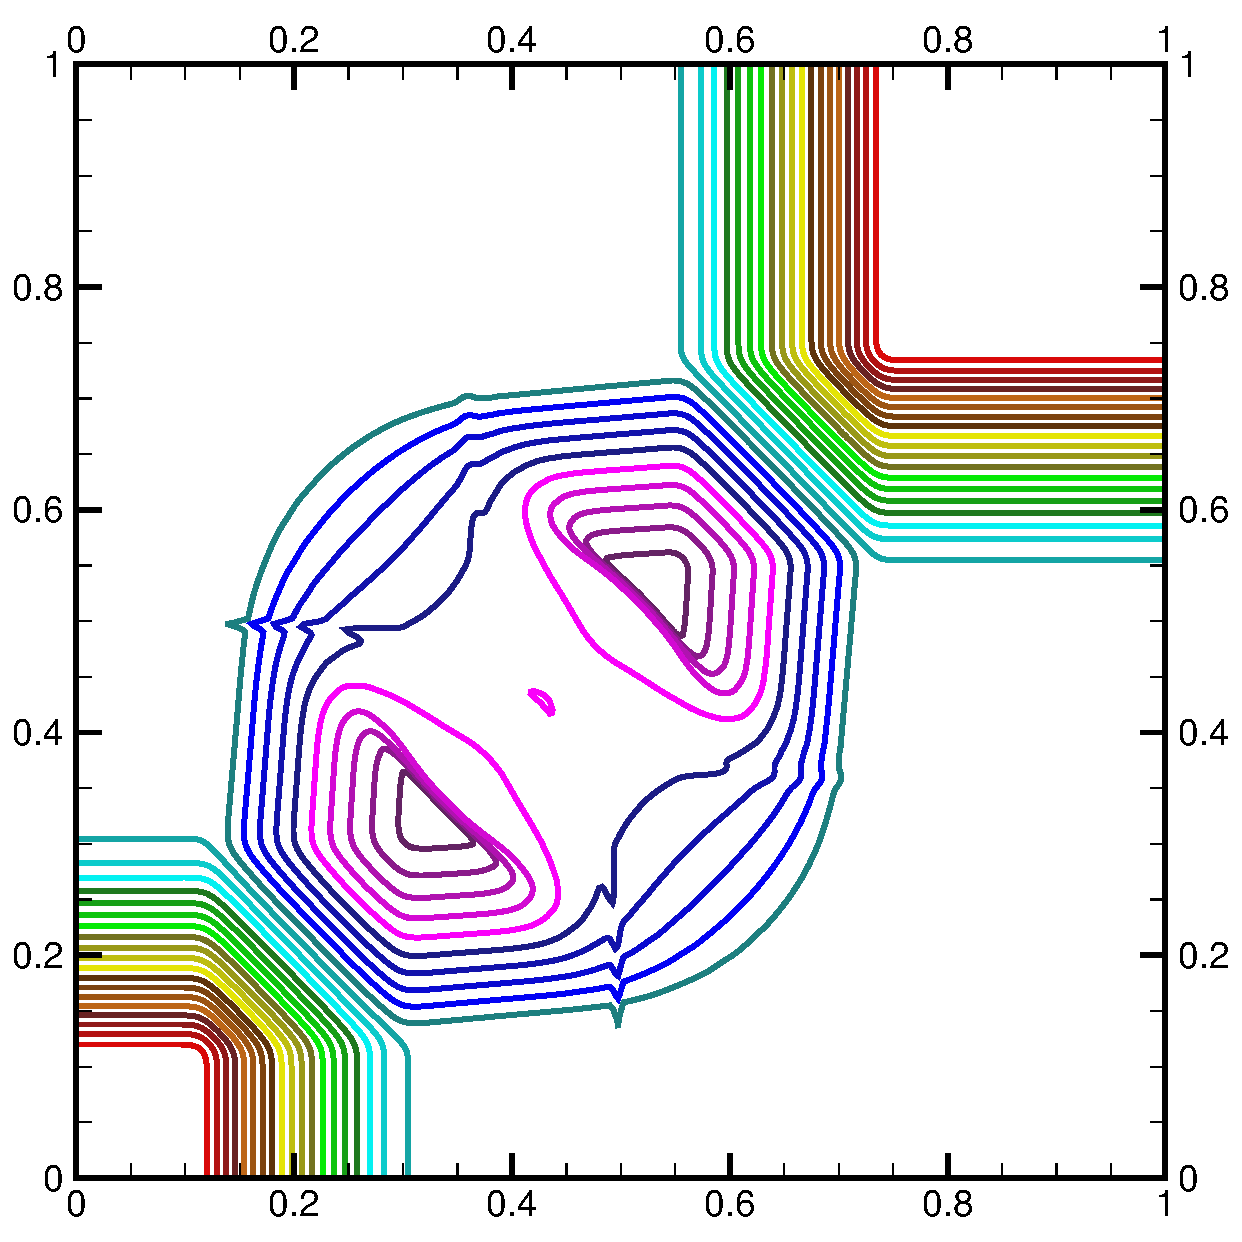
\includegraphics[height=0.4\textheight]{fig/2D/RP14_S2O4-WHC4_CFL0.600000.pdf}
%       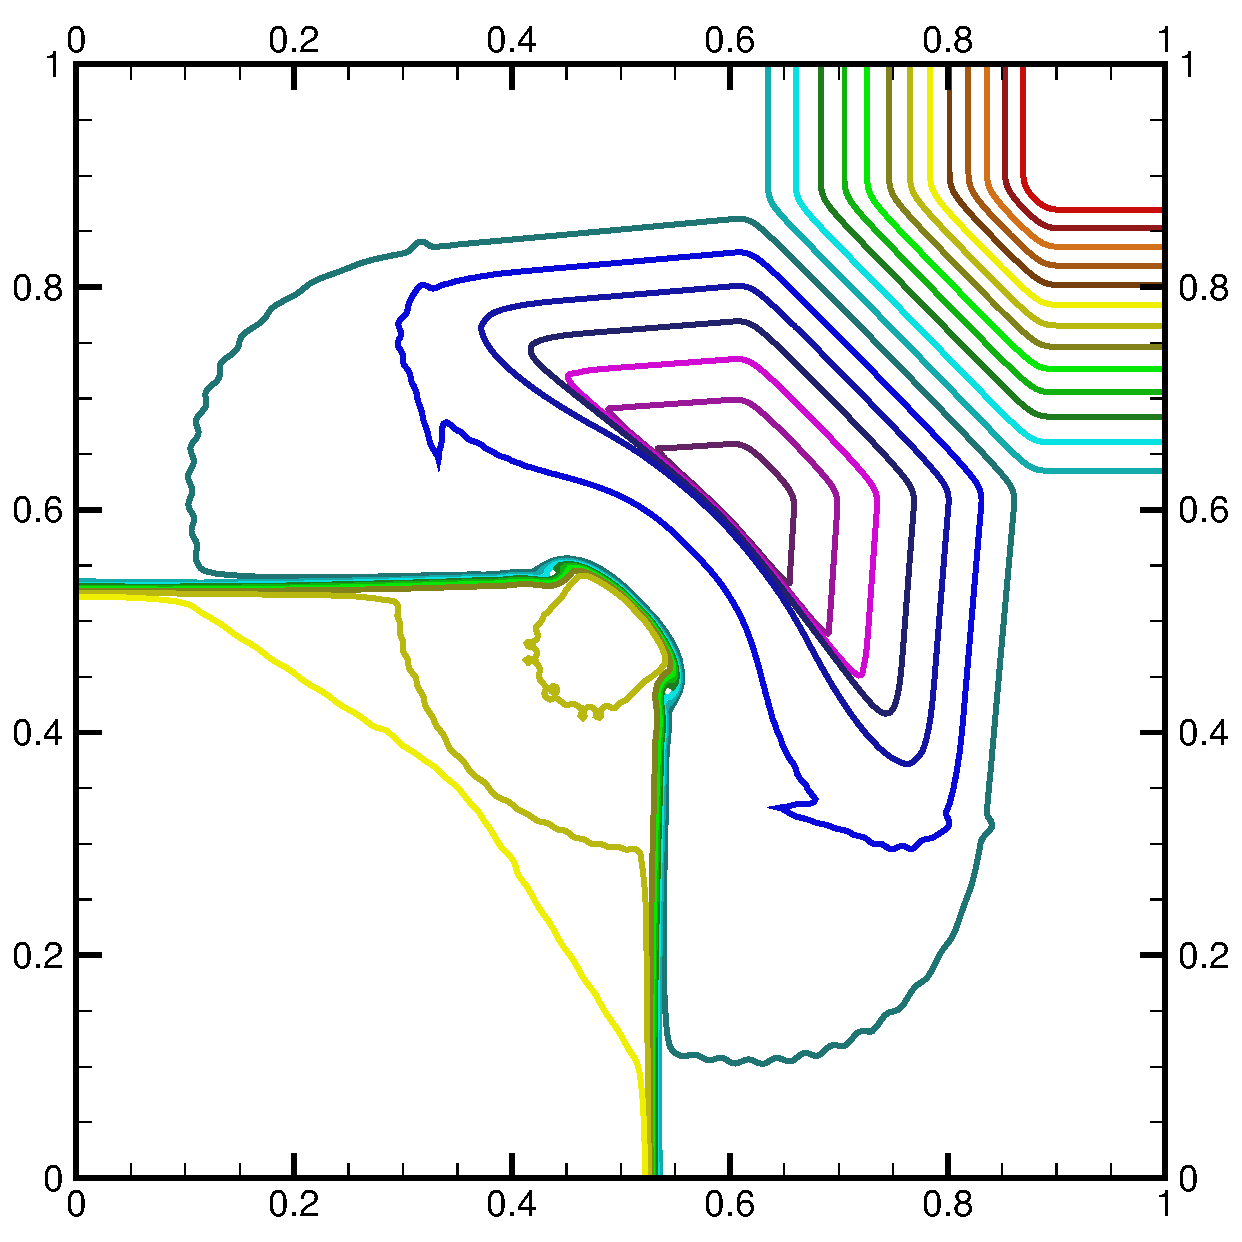
\includegraphics[height=0.4\textheight]{fig/2D/RP15_S2O4-WHC4_CFL0.600000.pdf}
%     \end{multicols}

%     \begin{multicols}{4}
%       \begin{minipage}{0.25\textwidth}
%         \vspace{0.1\textheight}
%         \centerline{HHC-4格式}
%       \end{minipage}
%       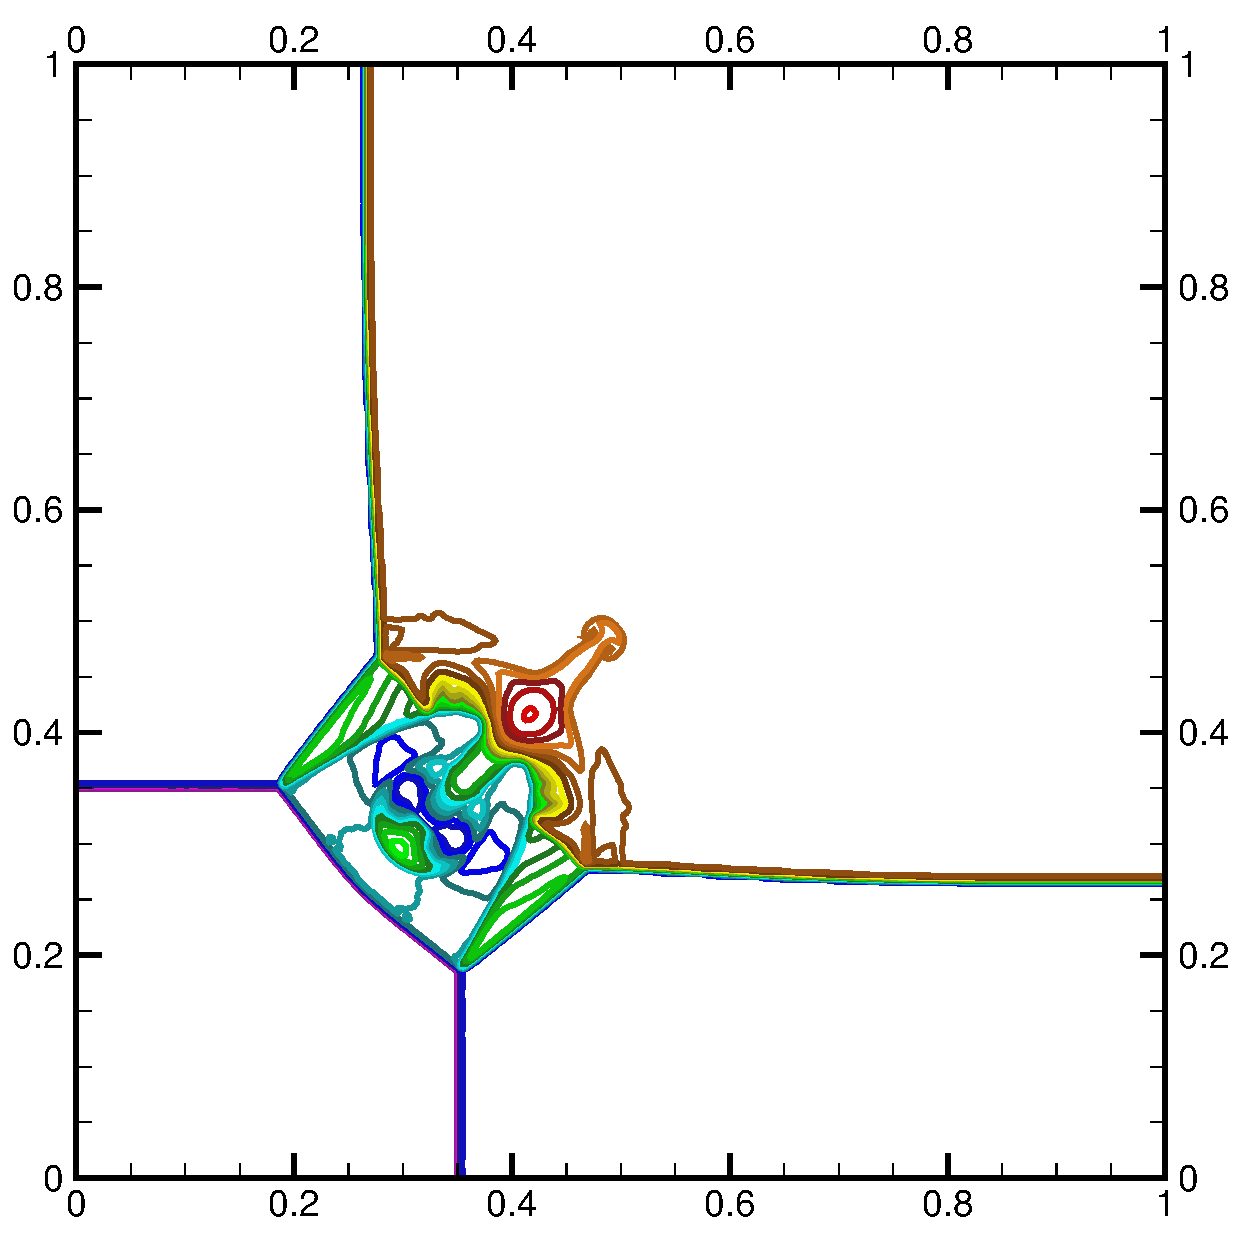
\includegraphics[height=0.4\textheight]{fig/2D/RP1_S2O4-HHC4theta20_CFL0.600000.pdf}
%       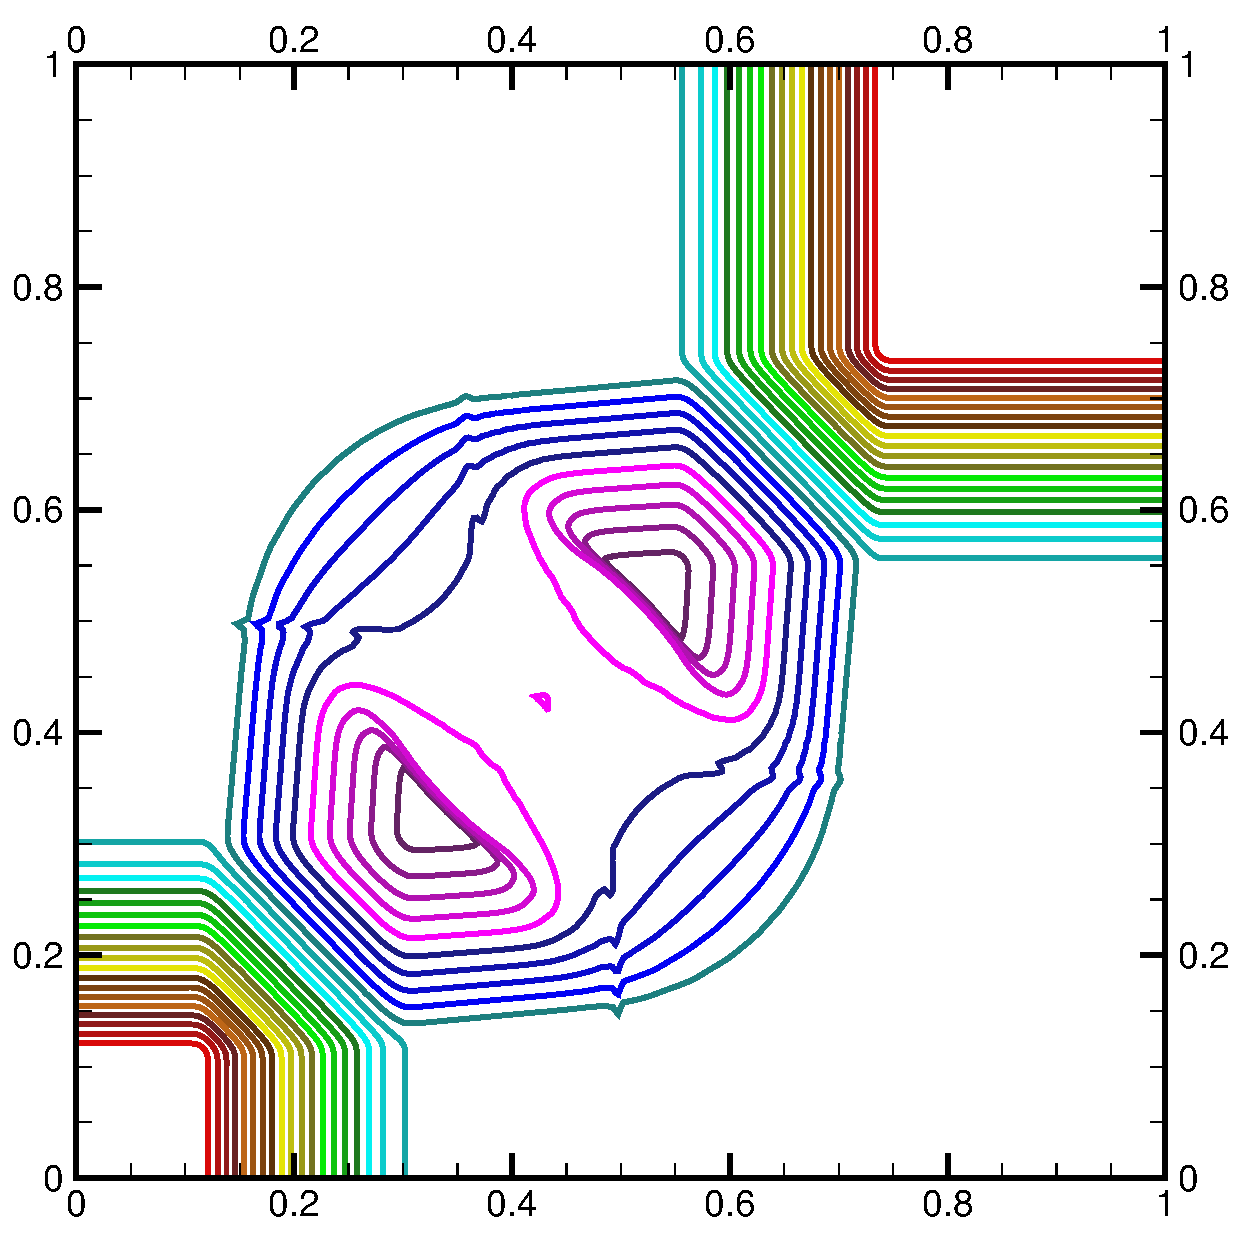
\includegraphics[height=0.4\textheight]{fig/2D/RP14_S2O4-HHC4theta20_CFL0.600000.pdf}
%       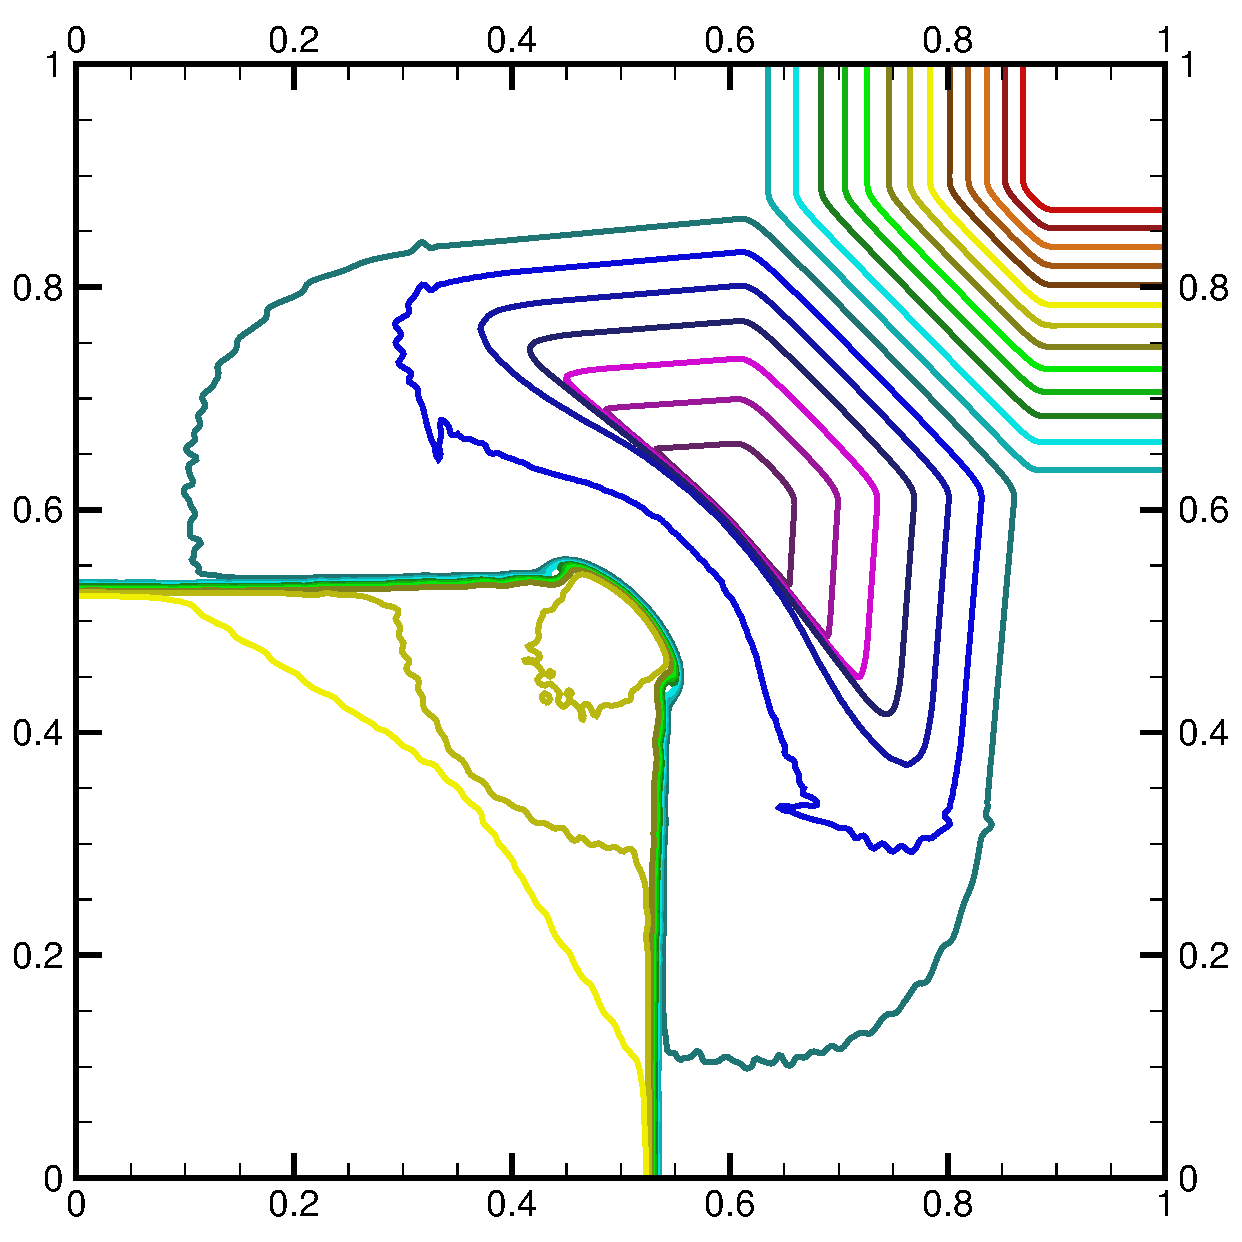
\includegraphics[height=0.4\textheight]{fig/2D/RP15_S2O4-HHC4theta20_CFL0.600000.pdf}
%     \end{multicols}
%   \end{figure}

% \end{frame}

\begin{frame}{二维欧拉方程组的黎曼问题1}
  
  \begin{example}[二维欧拉方程组的黎曼问题1]
    \label{ex:RP1}
    这是一个文 \citep{RPexample} 中提出的包含四个激波相互作用的算例,
    以欧拉方程组作为模型。
    计算区域是$[0,1]\times[0,1]$,
    初始条件是
    \begin{equation*}
      (\rho, u, v, p) (x, y)=
      \begin{cases}
        (1.5, 0, 0, 1.5),             & x>0.5,~y>0.5,  \\
        (0.532, 1.206, 0, 0.3),       & x<0.5,~y>0.5,  \\
        (0.138, 1.206, 1.206, 0.029), & x<0.5,~y<0.5,  \\
        (0.532, 0, 1.206, 0.3),       & x>0.5,~y<0.5.
      \end{cases}
    \end{equation*}
  \end{example}
  
\end{frame}

\begin{frame}{二维欧拉方程组的黎曼问题1的结果($400 \times 400$个网格,$t^{tem}=0.35$)}
  
  \begin{figure}[htbp]
    \centering
    \subfigure[WHC-4格式]{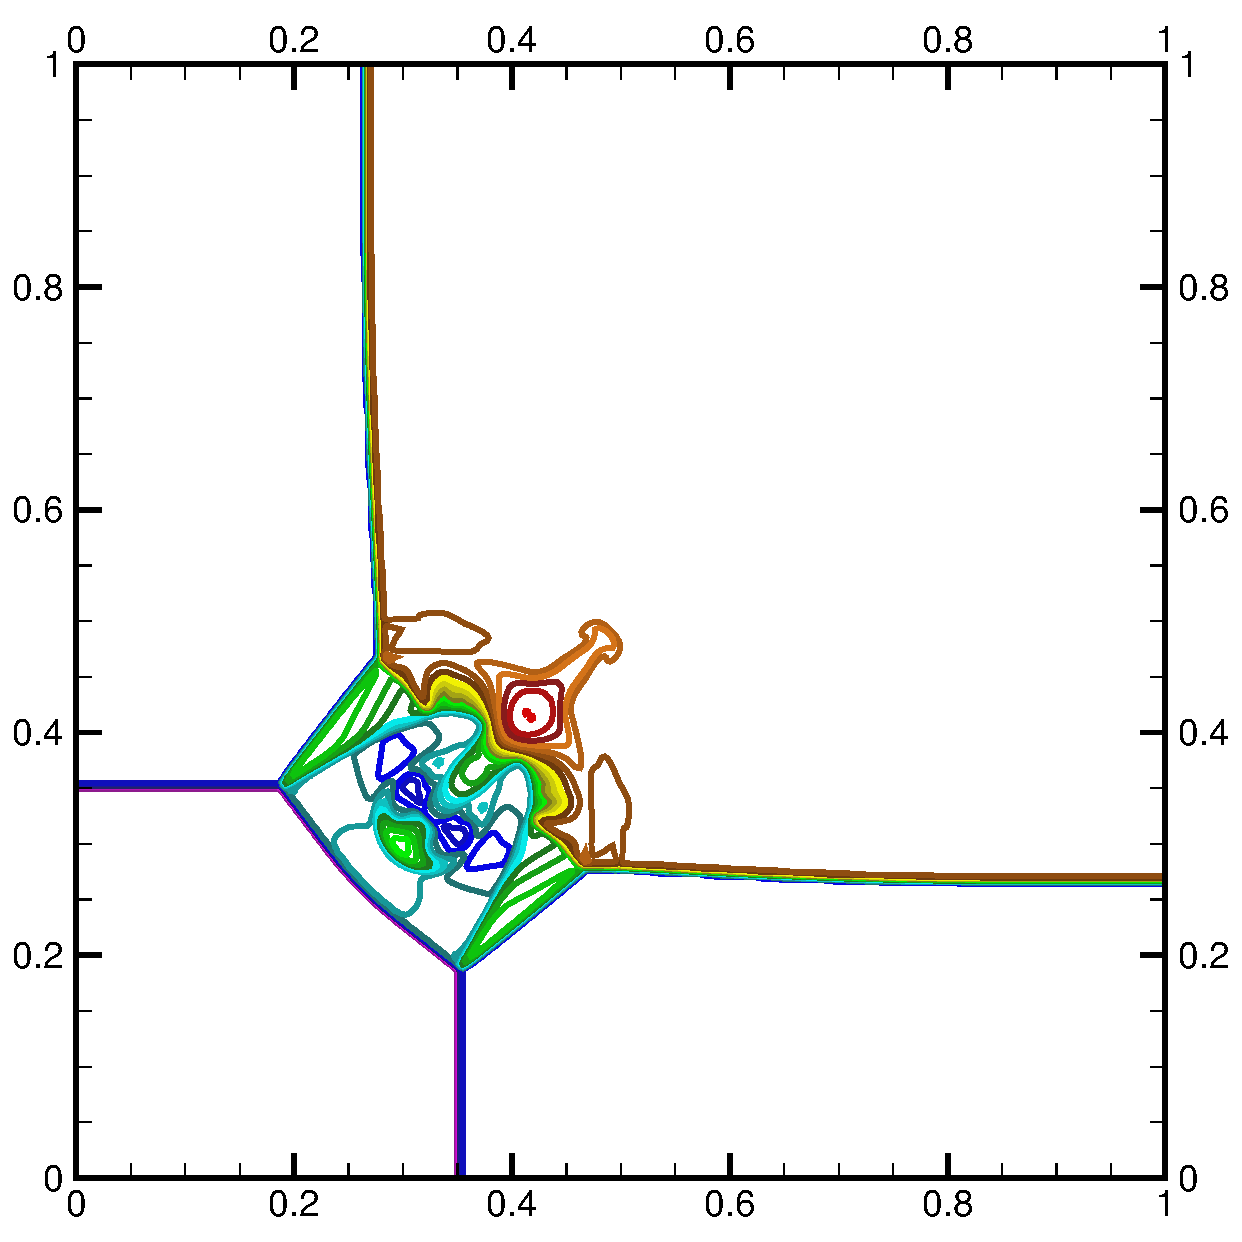
\includegraphics[width=0.43\textwidth]{fig/2D/RP1_S2O4-WHC4_CFL0.600000.pdf}}
    \hspace{0.05\textwidth}
    \subfigure[HHC-4格式]{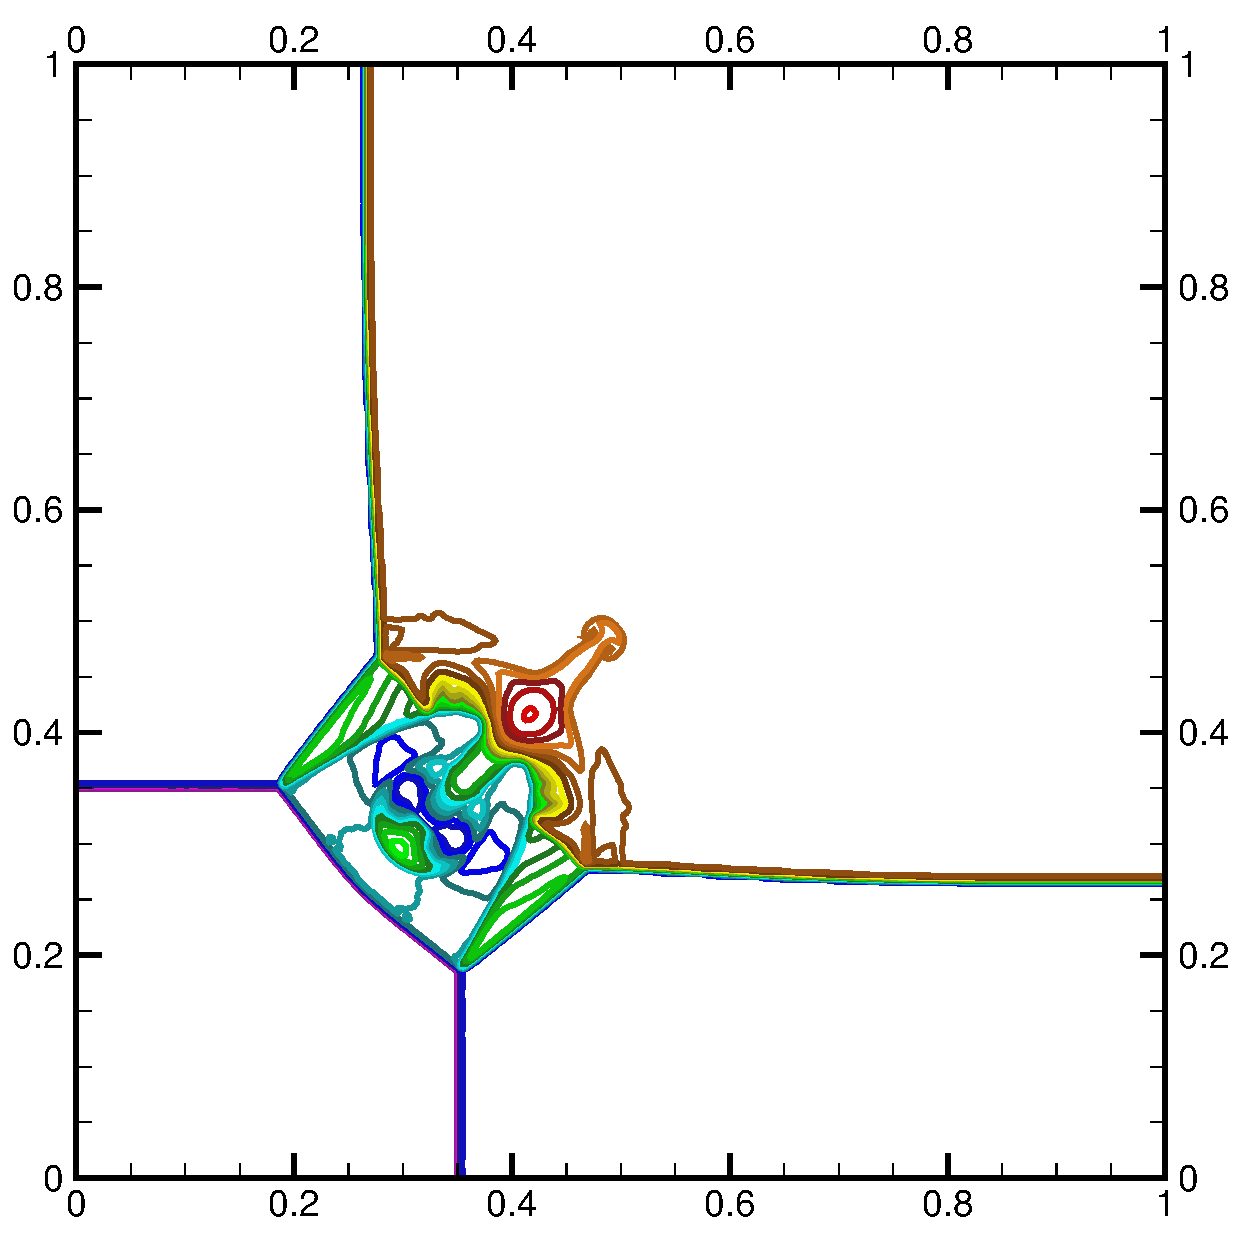
\includegraphics[width=0.43\textwidth]{fig/2D/RP1_S2O4-HHC4theta20_CFL0.600000.pdf}}
  \end{figure}
  
\end{frame}

\begin{frame}{二维欧拉方程组的黎曼问题2}
  
  \begin{example}[二维欧拉方程组的黎曼问题2]
    \label{ex:RP2}
    这是一个来自文 \citep{RPexample} 中的算例,
    以欧拉方程组作为模型,
    涉及到四个稀疏波的相互作用。
    计算区域是$[0,1]\times[0,1]$,
    初始条件如下
    \begin{equation*}
      (\rho, u, v, p) (x, y)=
      \begin{cases}
        (1, 0, 0, 1),           & x>0.5,~y>0.5,  \\
        (0.52, -0.726, 0, 0.4), & x<0.5,~y>0.5,  \\
        (1, -0.726, -0.726, 1), & x<0.5,~y<0.5,  \\
        (0.52, 0, -0.726, 0.4), & x>0.5,~y<0.5.
      \end{cases}
    \end{equation*}
  \end{example}
  
\end{frame}

\begin{frame}{二维欧拉方程组的黎曼问题2的结果($400 \times 400$个网格,$t^{tem}=0.2$)}
  
  \begin{figure}[htbp]
    \centering
    \subfigure[WHC-4格式]{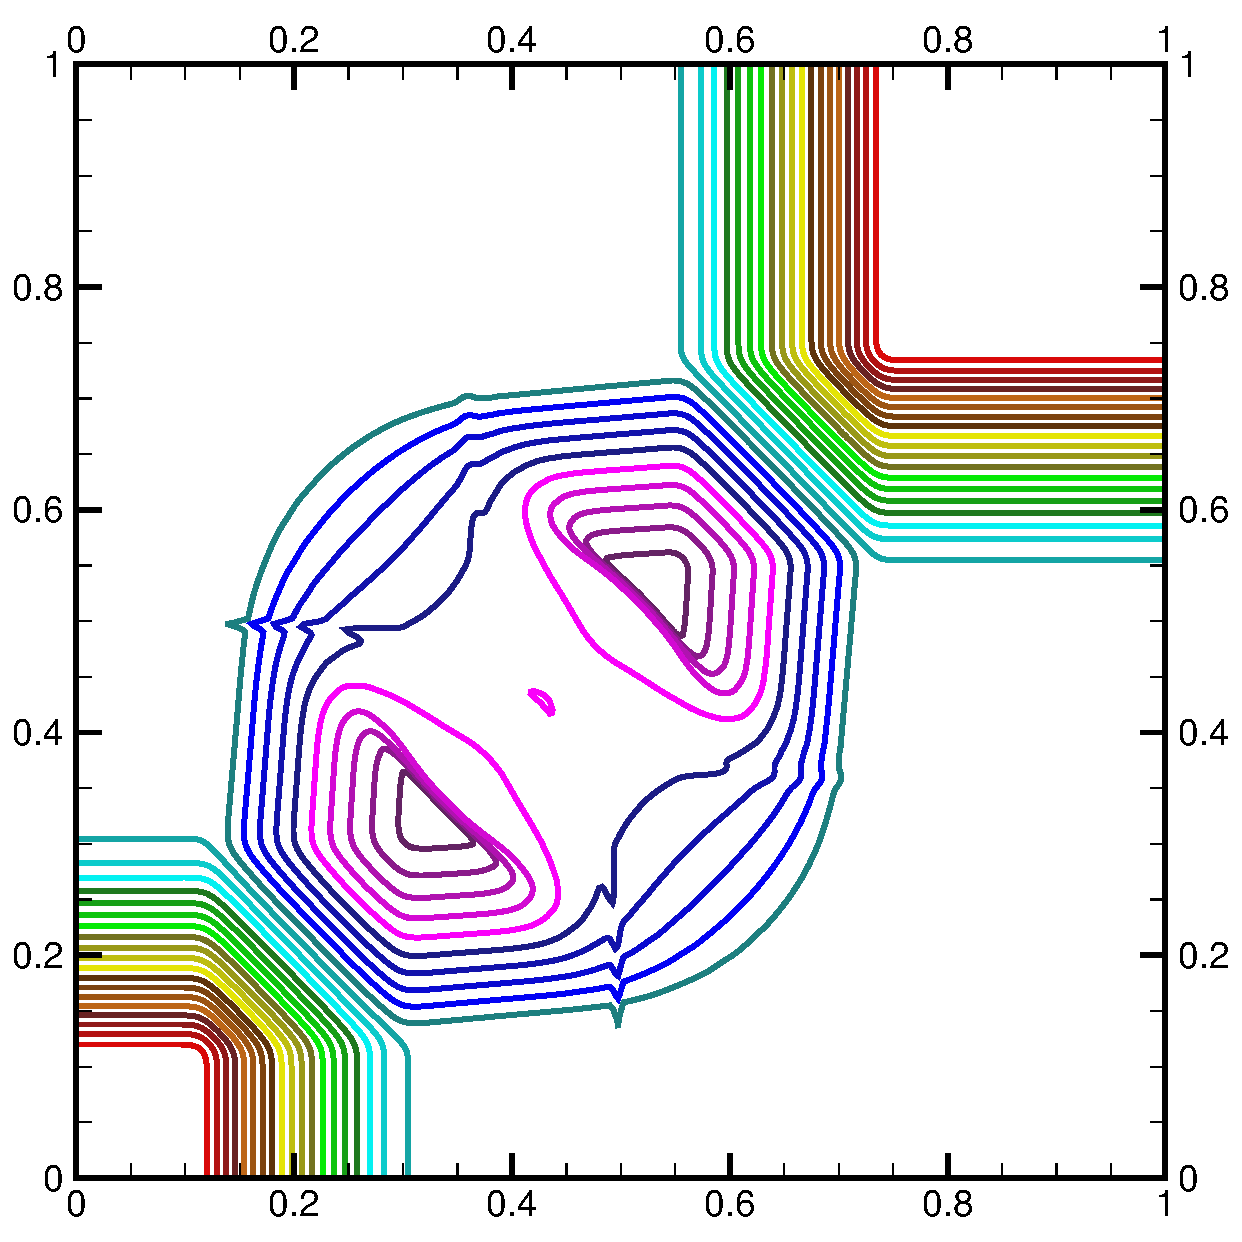
\includegraphics[width=0.43\textwidth]{fig/2D/RP14_S2O4-WHC4_CFL0.600000.pdf}}
    \hspace{0.05\textwidth}
    \subfigure[HHC-4格式]{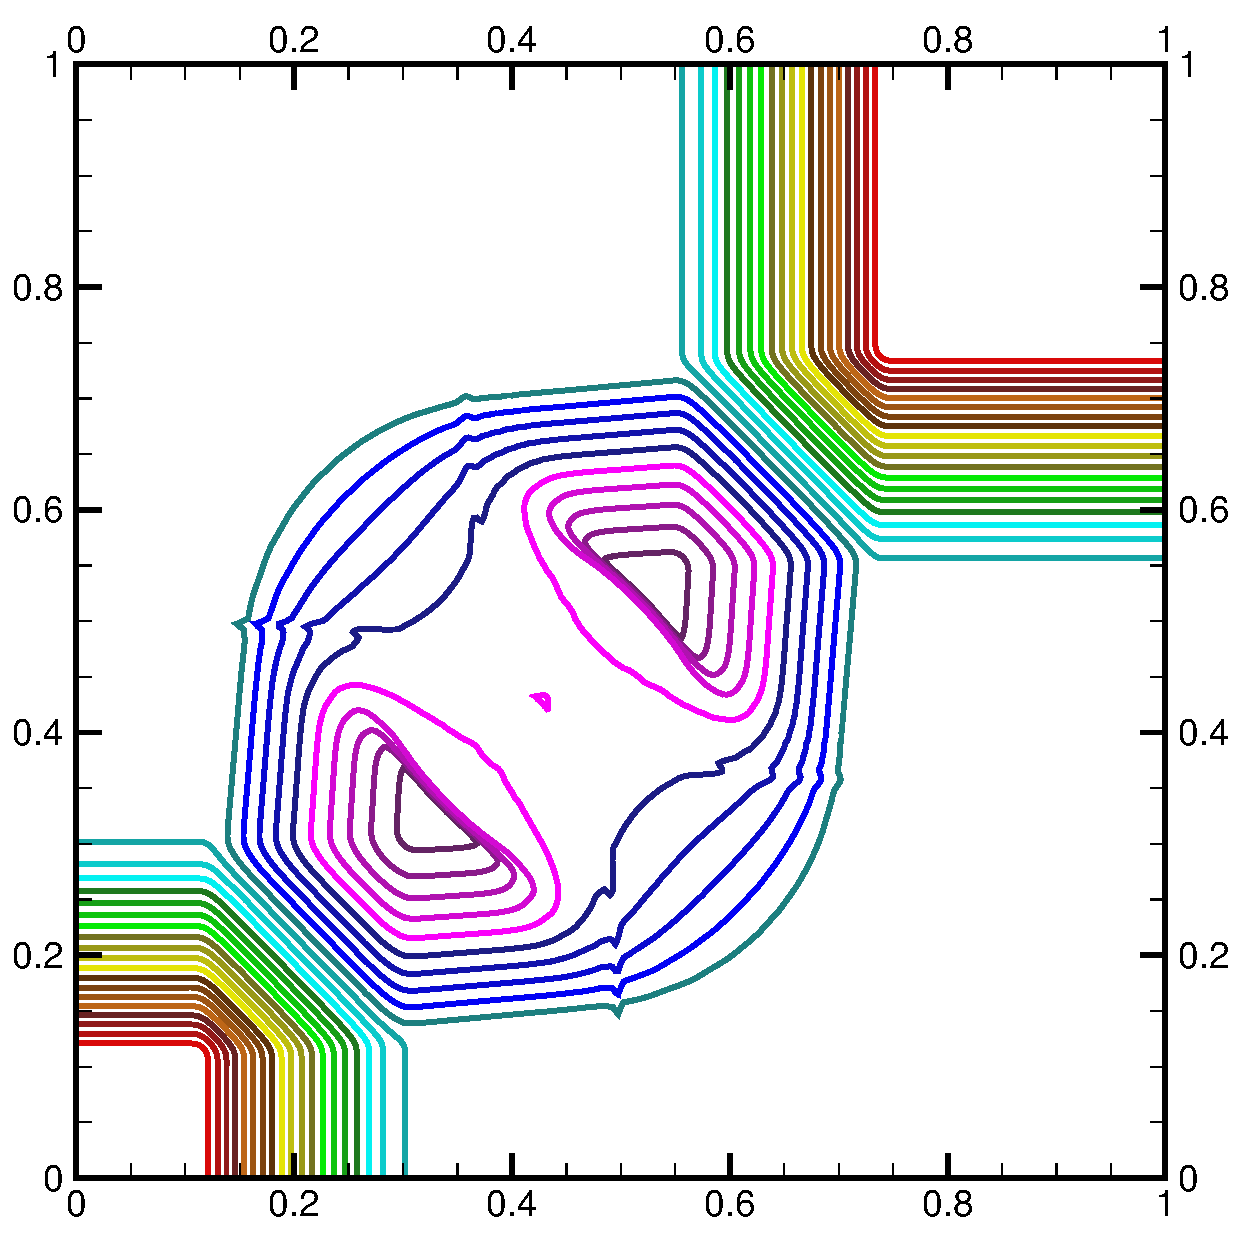
\includegraphics[width=0.43\textwidth]{fig/2D/RP14_S2O4-HHC4theta20_CFL0.600000.pdf}}
  \end{figure}
  
\end{frame}

\begin{frame}{二维欧拉方程组的黎曼问题3}
  
  \begin{example}[二维欧拉方程组的黎曼问题3]
    \label{ex:RP3}
    这是另一个来自文 \citep{RPexample} 中的算例,
    以欧拉方程组作为模型,
    涉及稀疏波和涡片的相互作用。
    计算区域也是$[0,1]\times[0,1]$,
    初始条件是
    \begin{equation*}
      (\rho, u, v, p) (x, y)=
      \begin{cases}
        (1, 0.1, 0.1, 1),         & x>0.5,~y>0.5,  \\
        (0.52, -0.626, 0.1, 0.4), & x<0.5,~y>0.5,  \\
        (0.8, 0.1, 0.1, 0.4),     & x<0.5,~y<0.5,  \\
        (0.52, 0.1, -0.626, 0.4), & x>0.5,~y<0.5.
      \end{cases}
    \end{equation*}
  \end{example}
  
\end{frame}

\begin{frame}{二维欧拉方程组的黎曼问题3的结果($400 \times 400$个网格,$t^{tem}=0.3$)}
  
  \begin{figure}[htbp]
    \centering
    \subfigure[WHC-4格式]{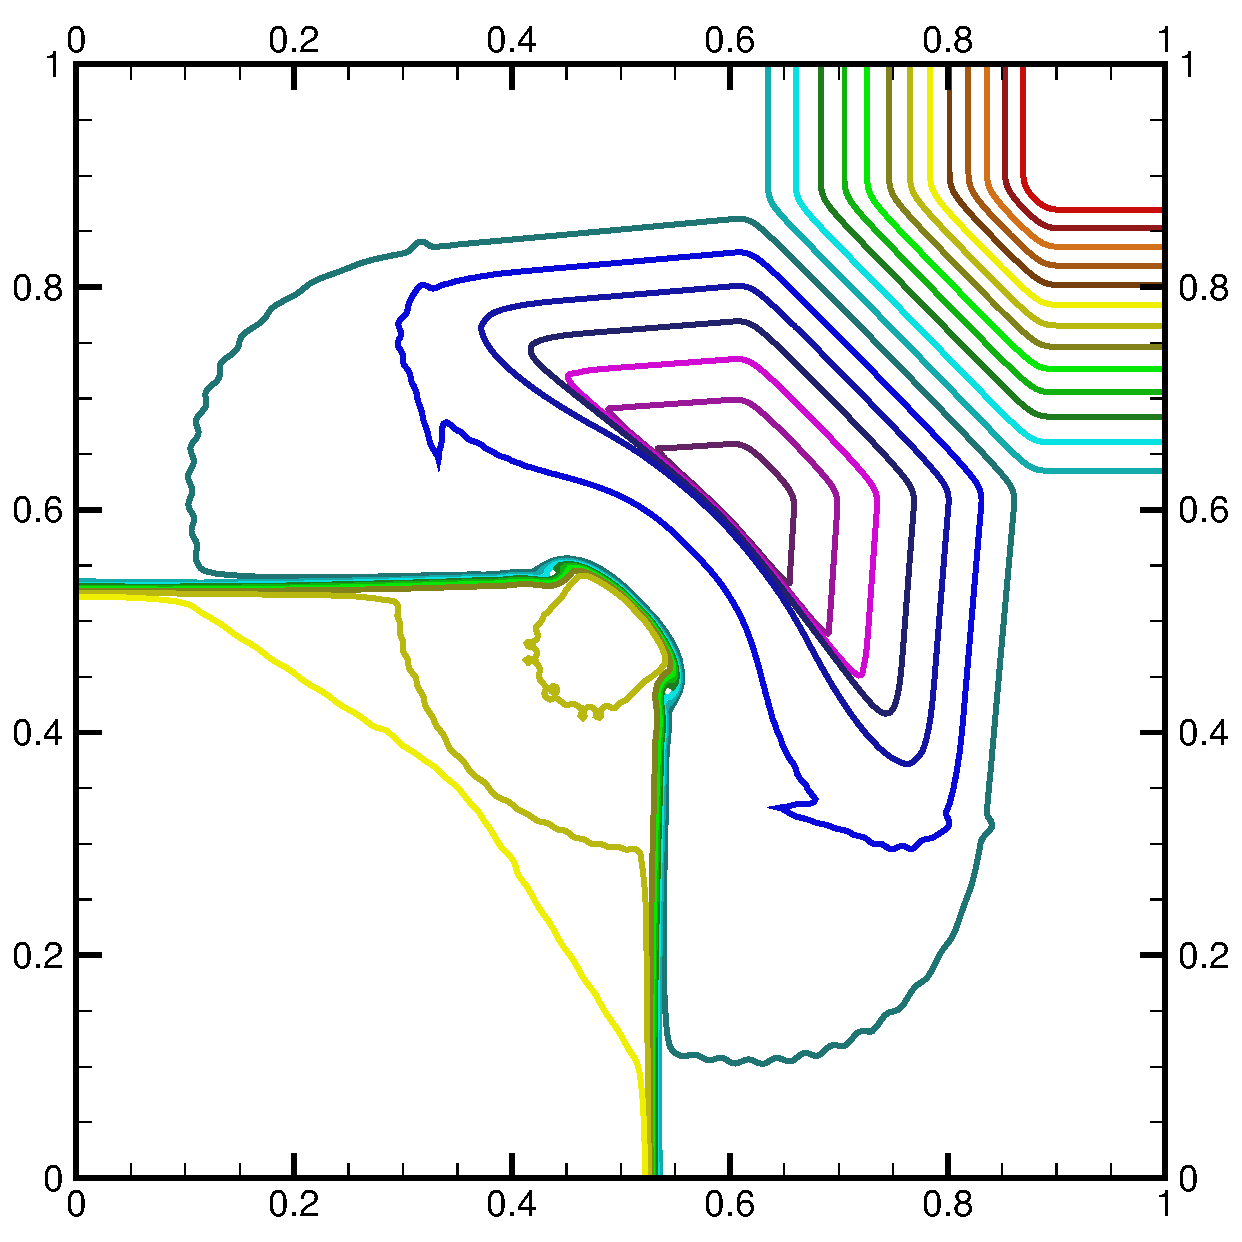
\includegraphics[width=0.43\textwidth]{fig/2D/RP15_S2O4-WHC4_CFL0.600000.pdf}}
    \hspace{0.05\textwidth}
    \subfigure[HHC-4格式]{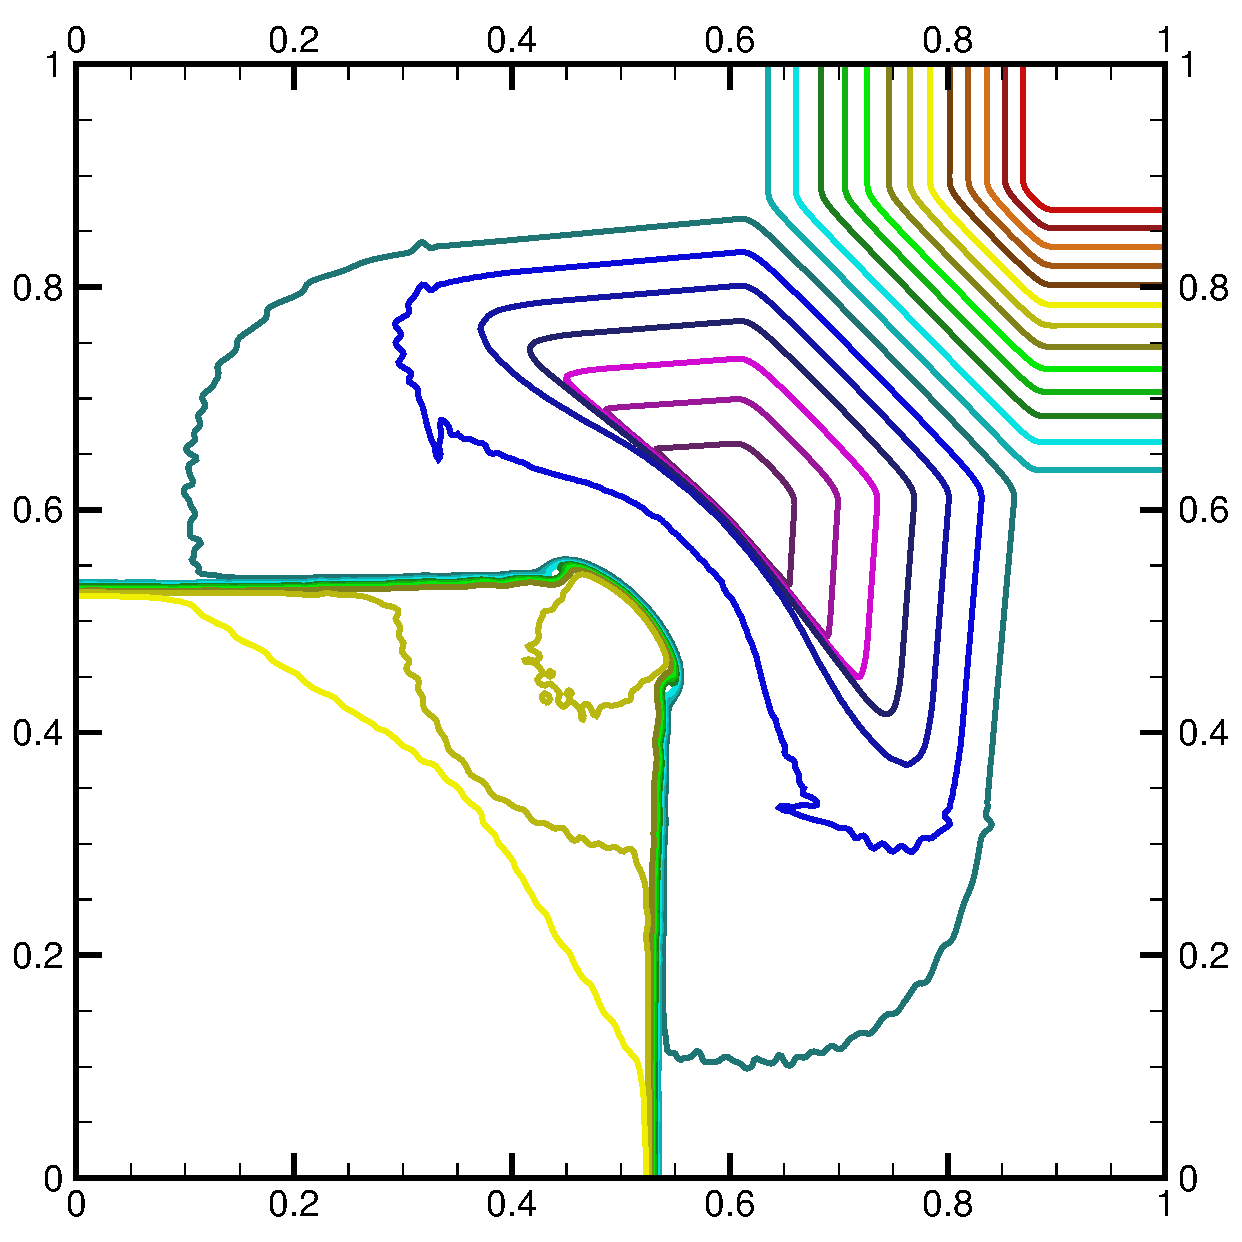
\includegraphics[width=0.43\textwidth]{fig/2D/RP15_S2O4-HHC4theta20_CFL0.600000.pdf}}
  \end{figure}
  
\end{frame}

\begin{frame}{二维欧拉方程组的双马赫反射问题}
  
  \begin{example}[二维欧拉方程组的双马赫反射问题]
    \label{ex:DoubleMach}
    这是一个经典的测试算例,
    以欧拉方程组作为模型。
    一个斜向激波撞击下方的反射边界,
    激波后状态是${\bm u}_L$,
    激波前状态为${\bm u}_R$,
    它们是
    \begin{align*}
      {\bm u}_L & =(\rho_L, u_L, v_L, p_L)= (8, 4.125\sqrt{3}, -4.125, 116.5), \\
      {\bm u}_R & =(\rho_R, u_R, v_R, p_R)= (1.4, 0, 0, 1).
    \end{align*}
    马赫数为10,
    计算区域为$[0,4]\times[0,1]$。
  \end{example}
  
\end{frame}

\begin{frame}{欧拉方程组的双马赫反射问题结果($1440 \times 360$个网格,$t^{tem}=0.2$)}
  
  \vspace{-4mm}
  \begin{figure}[htbp]
    \centering
    
    \begin{multicols}{8}
      \begin{minipage}{0.25\textwidth}
        \vspace{0.1\textheight}
        WHC-4\\格式
      \end{minipage}
      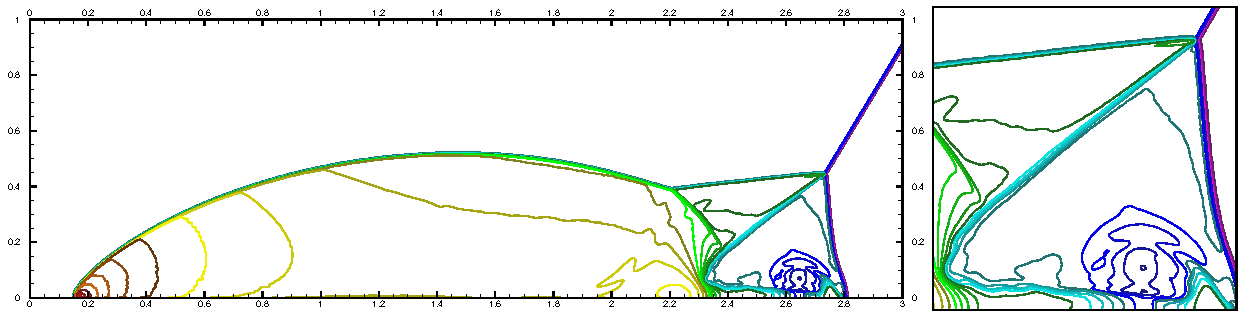
\includegraphics[height=0.4\textheight]{fig/2D/DoubleMach_S2O4-WHC4_CFL0.600000.pdf}
    \end{multicols}
    
    \begin{multicols}{8}
      \begin{minipage}{0.25\textwidth}
        \vspace{0.14\textheight}
        HHC-4\\格式
      \end{minipage}
      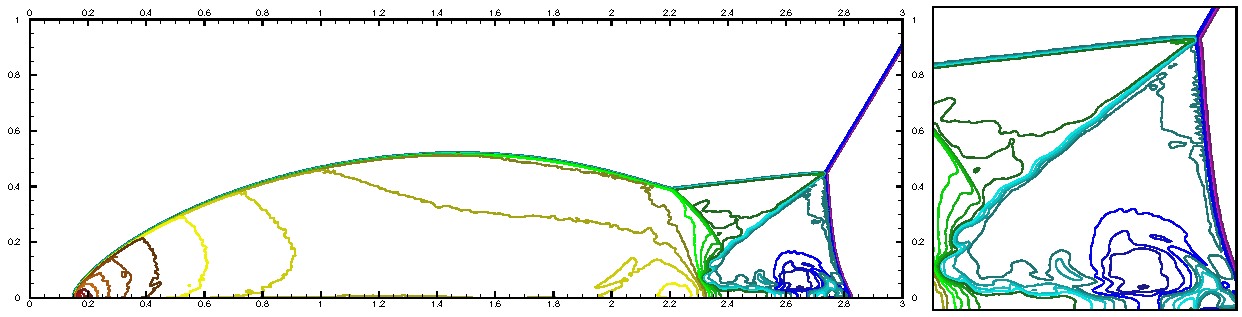
\includegraphics[height=0.4\textheight]{fig/2D/DoubleMach_S2O4-HHC4theta20_CFL0.600000.pdf}
    \end{multicols}
  \end{figure}
  
\end{frame}

\begin{frame}{二维欧拉方程组的前台阶问题}
  
  \begin{example}[二维欧拉方程组的前台阶问题]
    \label{ex:Frontstep}
    前台阶问题是一个经典的测试算例,
    以欧拉方程组作为模型,
    描述了一个带有台阶的管道,
    最初填充的是均匀的马赫数为$3$的均匀流体,
    其状态是
    \begin{equation*}
      (\rho, u, v, p)= (1.4, 3, 0, 1).
    \end{equation*}
    管道的壁面都是反射边界,
    而左侧和右侧分别作为流入和流出边界。
  \end{example}
  
\end{frame}

\begin{frame}{二维欧拉方程组的前台阶问题结果($480 \times 160$个网格,$t^{tem}=4$)}
  
  \vspace{-4mm}
  \begin{figure}[htbp]
    \centering
    
    \begin{multicols}{4}
      \begin{minipage}{0.25\textwidth}
        \vspace{0.1\textheight}
        \centerline{WHC-4格式}
      \end{minipage}
      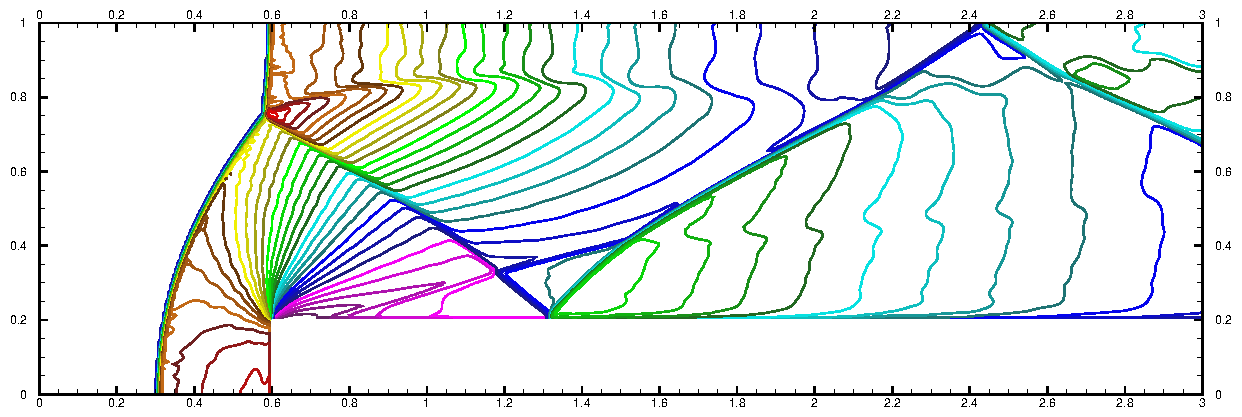
\includegraphics[height=0.4\textheight]{fig/2D/Frontstep_S2O4-WHC4_CFL0.600000.pdf}
    \end{multicols}
    
    \begin{multicols}{4}
      \begin{minipage}{0.25\textwidth}
        \vspace{0.14\textheight}
        \centerline{HHC-4格式}
      \end{minipage}
      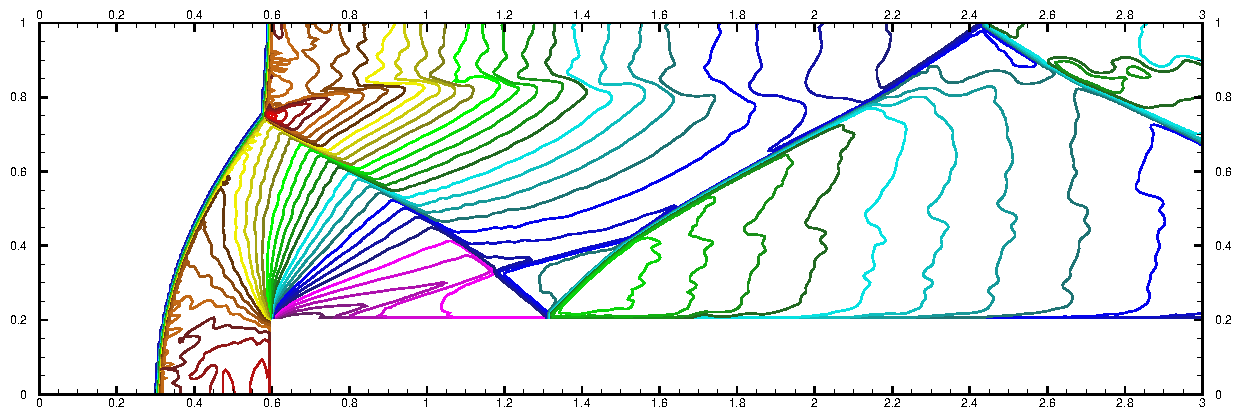
\includegraphics[height=0.4\textheight]{fig/2D/Frontstep_S2O4-HHC4theta20_CFL0.600000.pdf}
    \end{multicols}
  \end{figure}
  
\end{frame}

\subsection{空间八阶精度格式及其数值实验}

\begin{frame}{WHC-8和HHC-8格式}
  
  得到空间八阶的两步四阶格式的步骤:
  
  \begin{itemize}[<+->]
    \item 用从八阶线性重构导出的多项式替换四阶线性重构导出的多项式
    \item 重新计算相应的光滑因子
    \item 调整格式中的参数(WHC-8格式中的$q=3$和HHC-8格式中的$\bar\vartheta=200000$)
  \end{itemize}
  
\end{frame}

\begin{frame}{二维欧拉方程组的线性退化的精度测试结果}
  
  \vspace{-3mm}
  \begin{columns}
    \begin{column}{0.2\textwidth}
      
      \centering
      
      WHC-8格式
      
      \vspace{0.4\textheight}
      
      HHC-8格式
      
    \end{column}
    \begin{column}{0.8\textwidth}
      \begin{tiny}
        \def\titleintable{CFL&$h$&Nstep&$L^1$-error&$L^1$-order&$L^\infty$-error&$L^\infty$-order\\}
% \begin{table}[htbp]
%   \caption{HC-2格式在\cref{ex:2D-acc2-re} 中密度的$L^1$和$L^\infty$误差和误差阶。展示的是$t^{tem} = 2$时刻的结果。}
%   \label{ta:2D-ex2-HC2}
%   \centering
%   \begin{tabular}{ccccccc}
%     \toprule
%     \titleintable
%     \midrule
%     0.6 & 2/10 & 48       & 1.11763e-02 &          & 1.72683e-02 &          \\
%     0.6 & 2/20 & 96       & 3.01412e-03 & 1.89063  & 4.66571e-03 & 1.88796  \\
%     0.6 & 2/40 & 235      & 2.61041     & -9.75832 & 949.546     & -17.6348 \\
%     0.6 & 2/80 & $\infty$ & -           & -        & -           & -        \\
%     \bottomrule
%   \end{tabular}
% \end{table}

% \begin{table}[htbp]
%   \caption{GRP格式在\cref{ex:2D-acc2-re} 中密度的$L^1$和$L^\infty$误差和误差阶。展示的是$t^{tem} = 2$时刻的结果。}
%   \label{ta:2D-ex2-GRP}
%   \centering
%   \begin{tabular}{ccccccc}
%     \toprule
%     \titleintable
%     \midrule
%     0.6 & 2/10  & 47   & 5.00978e-02 &         & 8.58273e-02 &         \\
%     0.6 & 2/20  & 95   & 1.67012e-02 & 1.58480 & 4.08864e-02 & 1.06982 \\
%     0.6 & 2/40  & 191  & 7.52718e-03 & 1.14977 & 1.78862e-02 & 1.19278 \\
%     0.6 & 2/80  & 383  & 2.14303e-03 & 1.81246 & 7.55058e-03 & 1.24418 \\
%     0.6 & 2/160 & 765  & 5.98699e-04 & 1.83975 & 3.10497e-03 & 1.28201 \\
%     0.6 & 2/320 & 1531 & 1.62786e-04 & 1.87885 & 1.26034e-03 & 1.30077 \\
%     \bottomrule
%   \end{tabular}
% \end{table}

\begin{table}[htbp]
  \caption{HC-8格式在\cref{ex:2D-acc2-re} 中密度的$L^1$和$L^\infty$误差和误差阶。展示的是$t^{tem} = 2$时刻的结果。}
  \label{ta:2D-ex2-HC8}
  \centering
  \begin{tabular}{ccccccc}
    \toprule
    \titleintable
    \midrule
    0.5   & 2/10 & 58  & 1.66073e-05 &         & 2.56597e-05 &         \\
    0.25  & 2/20 & 230 & 8.13500e-08 & 7.67346 & 1.25816e-07 & 7.67204 \\
    \midrule
    0.5   & 2/20 & 115 & 1.60981e-07 &         & 2.52335e-07 &         \\
    0.25  & 2/40 & 460 & 6.74489e-10 & 7.89888 & 1.05654e-09 & 7.89984 \\
    \midrule
    0.5   & 2/40 & 230 & 4.93010e-09 &         & 7.75582e-09 &         \\
    0.333 & 2/60 & 517 & 1.97526e-10 & 7.93469 & 3.10969e-10 & 7.93288 \\
    \midrule
    0.5   & 2/60 & 345 & 6.58714e-10 &         & 1.03541e-09 &         \\
    0.375 & 2/80 & 613 & 6.73304e-11 & 7.92777 & 1.06740e-10 & 7.89813 \\
    % \midrule
    % 0.5 & 2/80 & 460 & 1.58708e-10 & & 2.50708e-10 & \\
    % 0.4 & 2/100 & 718 & 2.70813e-11 & 7.92414 & 4.44493e-11 & 7.75258 \\
    % \midrule
    % 0.5 & 2/100 & 575 & 5.29640e-11 & & 8.46452e-11 & \\
    % 0.417 & 2/120 & 827 & 1.24968e-11 & 7.92083 & 2.28260e-11 & 7.18823 \\
    \bottomrule
  \end{tabular}
\end{table}

\begin{table}[htbp]
  \caption{WHC-8格式在\cref{ex:2D-acc2-re} 中密度的$L^1$和$L^\infty$误差和误差阶。展示的是$t^{tem} = 2$时刻的结果。}
  \label{ta:2D-ex2-WHC8}
  \centering
  \begin{tabular}{ccccccc}
    \toprule
    \titleintable
    \midrule
    0.500 & 2/10 & 58  & 1.65877e-05 &         & 2.56825e-05 &         \\
    0.250 & 2/20 & 230 & 8.08424e-08 & 7.68079 & 1.27776e-07 & 7.65103 \\
    \midrule
    0.500 & 2/20 & 115 & 1.60989e-07 &         & 2.50151e-07 &         \\
    0.250 & 2/40 & 460 & 6.76413e-10 & 7.89484 & 1.08095e-09 & 7.85435 \\
    \midrule
    0.500 & 2/40 & 230 & 4.92854e-09 &         & 7.6186e-09  &         \\
    0.333 & 2/60 & 517 & 1.97332e-10 & 7.93634 & 3.01551e-10 & 7.96470 \\
    \midrule
    0.500 & 2/60 & 345 & 6.57423e-10 &         & 9.96912e-10 &         \\
    0.375 & 2/80 & 613 & 6.71483e-11 & 7.93037 & 1.10485e-10 & 7.64659 \\
    \bottomrule
  \end{tabular}
\end{table}

\begin{table}[htbp]
  \caption{HHC-8格式在\cref{ex:2D-acc2-re} 中密度的$L^1$和$L^\infty$误差和误差阶。展示的是$t^{tem} = 2$时刻的结果。}
  \label{ta:2D-ex2-HHC8}
  \centering
  \begin{tabular}{ccccccc}
    \toprule
    \titleintable
    \midrule
    0.5   & 2/10 & 58  & 1.66073e-05 &         & 2.56597e-05 &         \\
    0.25  & 2/20 & 230 & 8.13500e-08 & 7.67346 & 1.25816e-07 & 7.67204 \\
    \midrule
    0.5   & 2/20 & 115 & 1.60981e-07 &         & 2.52335e-07 &         \\
    0.25  & 2/40 & 460 & 6.74489e-10 & 7.89888 & 1.05654e-09 & 7.89984 \\
    \midrule
    0.5   & 2/40 & 230 & 4.93010e-09 &         & 7.75582e-09 &         \\
    0.333 & 2/60 & 517 & 1.97526e-10 & 7.93469 & 3.10969e-10 & 7.93288 \\
    \midrule
    0.5   & 2/60 & 345 & 6.58714e-10 &         & 1.03541e-09 &         \\
    0.375 & 2/80 & 613 & 6.73304e-11 & 7.92777 & 1.06740e-10 & 7.89813 \\
    \bottomrule
  \end{tabular}
\end{table}
\undef\titleintable
      \end{tiny}
    \end{column}
  \end{columns}
  
\end{frame}

\begin{frame}{二维欧拉方程组的非线性的精度测试结果}
  
  \vspace{-3mm}
  \begin{columns}
    \begin{column}{0.2\textwidth}
      
      \centering
      
      WHC-8格式
      
      \vspace{0.4\textheight}
      
      HHC-8格式
      
    \end{column}
    \begin{column}{0.8\textwidth}
      \begin{tiny}
        \def\titleintable{CFL&$h$&Nstep&$L^1$-error&$L^1$-order&$L^\infty$-error&$L^\infty$-order\\}
% \begin{table}[htbp]
%   \caption{HC-2格式在例 \ref{ex:2D-acc3} 中$u$的$L^1$和$L^\infty$误差和误差阶。展示的是$t^{tem} = 1$时刻的结果。}
%   \label{ta:2D-ex3-HC2}
%   \centering
%   \begin{tabular}{ccccccc}
%     \toprule
%     \titleintable
%     \midrule
%     % 0.6 &$4\pi$/100 & 32 & 4.81945e-06 & & 1.01489e-05 & \\
%     % 0.6 &$4\pi$/150 & 48 & 2.14115e-06 & 2.00096 & 4.53644e-06 & 1.98592 \\
%     0.6 & $4\pi$/150 & 48  & 2.14115e-06 &         & 4.53644e-06 &         \\
%     0.6 & $4\pi$/200 & 64  & 1.20379e-06 & 2.00175 & 2.55650e-06 & 1.99354 \\
%     0.6 & $4\pi$/250 & 80  & 7.69947e-07 & 2.00277 & 1.63922e-06 & 1.99162 \\
%     0.6 & $4\pi$/300 & 96  & 5.34405e-07 & 2.00288 & 1.13914e-06 & 1.99620 \\
%     0.6 & $4\pi$/350 & 112 & 3.92411e-07 & 2.00352 & 8.37585e-07 & 1.99482 \\
%     0.6 & $4\pi$/400 & 128 & 3.00264e-07 & 2.00439 & 6.43520e-07 & 1.97383 \\
%     \bottomrule
%   \end{tabular}
% \end{table}

% \begin{table}[htbp]
%   \caption{HC-8格式在例 \ref{ex:2D-acc3} 中$u$的$L^1$和$L^\infty$误差和误差阶。展示的是$t^{tem} = 1$时刻的结果。}
%   \label{ta:2D-ex3-HC8}
%   \centering
%   \begin{tabular}{ccccccc}
%     \toprule
%     \titleintable
%     \midrule
%     0.5   & $4\pi$/100 & 39 & 8.82554e-10 &              & 4.69837e-09 &              \\
%     0.417 & $4\pi$/120 & 56 & 2.24268e-10 & \hl{7.51407} & 1.20324e-09 & \hl{7.47139} \\
%     \midrule
%     0.5   & $4\pi$/120 & 46 & 3.47755e-10 &              & 1.84389e-09 &              \\
%     0.429 & $4\pi$/140 & 63 & 1.09164e-10 & \hl{7.51635} & 5.92636e-10 & \hl{7.36325} \\
%     \midrule
%     0.5   & $4\pi$/140 & 54 & 1.60710e-10 &              & 8.36642e-10 &              \\
%     0.438 & $4\pi$/160 & 70 & 5.85239e-11 & \hl{7.56503} & 3.17302e-10 & \hl{7.26078} \\
%     \midrule
%     0.5   & $4\pi$/160 & 62 & 8.29972e-11 &              & 4.17968e-10 &              \\
%     0.444 & $4\pi$/180 & 78 & 3.40451e-11 & \hl{7.56579} & 1.83270e-10 & \hl{6.99968} \\
%     % \midrule
%     % 0.5 &$4\pi$/180 & 69 & 4.70364e-11 & & 2.33891e-10 & \\
%     % 0.45 &$4\pi$/200 & 85 & 2.11229e-11 & 7.59834 & 1.14002e-10 & 6.82077 \\
%     % \midrule
%     % 0.5 &$4\pi$/200 & 77 & 2.84649e-11 & & 1.39577e-10 & \\
%     % 0.4 &$4\pi$/250 & 120 & 5.68912e-12 & 7.21560 & 4.28886e-11 & 5.28812 \\
%     \bottomrule
%   \end{tabular}
% \end{table}

\begin{table}[htbp]
  % \caption{WHC-8格式在例 \ref{ex:2D-acc3} 中$u$的$L^1$和$L^\infty$误差和误差阶。展示的是$t^{tem} = 1$时刻的结果。}
  \label{ta:2D-ex3-WHC8}
  \centering
  \begin{tabular}{ccccccc}
    \toprule
    \titleintable
    \midrule
    0.5   & $4\pi$/100 & 39 & 8.82554e-10 &              & 4.69837e-09 &              \\
    0.417 & $4\pi$/120 & 56 & 2.24268e-10 & \hl{7.51407} & 1.20324e-09 & \hl{7.47139} \\
    \midrule
    0.5   & $4\pi$/120 & 46 & 3.47755e-10 &              & 1.84389e-09 &              \\
    0.429 & $4\pi$/140 & 63 & 1.09164e-10 & \hl{7.51635} & 5.92636e-10 & \hl{7.36325} \\
    \midrule
    0.5   & $4\pi$/140 & 54 & 1.60710e-10 &              & 8.36642e-10 &              \\
    0.438 & $4\pi$/160 & 70 & 5.85239e-11 & \hl{7.56503} & 3.17302e-10 & \hl{7.26078} \\
    \midrule
    0.5   & $4\pi$/160 & 62 & 8.29972e-11 &              & 4.17968e-10 &              \\
    0.444 & $4\pi$/180 & 78 & 3.40451e-11 & \hl{7.56579} & 1.83270e-10 & \hl{6.99968} \\
    \bottomrule
  \end{tabular}
\end{table}

\begin{table}[htbp]
  % \caption{HHC-8格式在例 \ref{ex:2D-acc3} 中$u$的$L^1$和$L^\infty$误差和误差阶。展示的是$t^{tem} = 1$时刻的结果。}
  \label{ta:2D-ex3-HHC8}
  \centering
  \begin{tabular}{ccccccc}
    \toprule
    \titleintable
    \midrule
    0.5   & $4\pi$/100 & 39 & 8.82554e-10 &              & 4.69837e-09 &              \\
    0.417 & $4\pi$/120 & 56 & 2.24268e-10 & \hl{7.51407} & 1.20324e-09 & \hl{7.47139} \\
    \midrule
    0.5   & $4\pi$/120 & 46 & 3.47755e-10 &              & 1.84389e-09 &              \\
    0.429 & $4\pi$/140 & 63 & 1.09164e-10 & \hl{7.51635} & 5.92636e-10 & \hl{7.36325} \\
    \midrule
    0.5   & $4\pi$/140 & 54 & 1.60710e-10 &              & 8.36642e-10 &              \\
    0.438 & $4\pi$/160 & 70 & 5.85239e-11 & \hl{7.56503} & 3.17302e-10 & \hl{7.26078} \\
    \midrule
    0.5   & $4\pi$/160 & 62 & 8.29972e-11 &              & 4.17968e-10 &              \\
    0.444 & $4\pi$/180 & 78 & 3.40451e-11 & \hl{7.56579} & 1.83270e-10 & \hl{6.99968} \\
    \bottomrule
  \end{tabular}
\end{table}
\undef\titleintable
      \end{tiny}
    \end{column}
  \end{columns}
  
\end{frame}

\begin{frame}{二维欧拉方程组的黎曼问题($300 \times 300$个网格)}
  
  \vspace{-4mm}
  \begin{figure}[htbp]
    \centering
    
    \begin{multicols}{4}
      \begin{minipage}{0.25\textwidth}
        \vspace{0.13\textheight}
        \centerline{WHC-4格式}
      \end{minipage}
      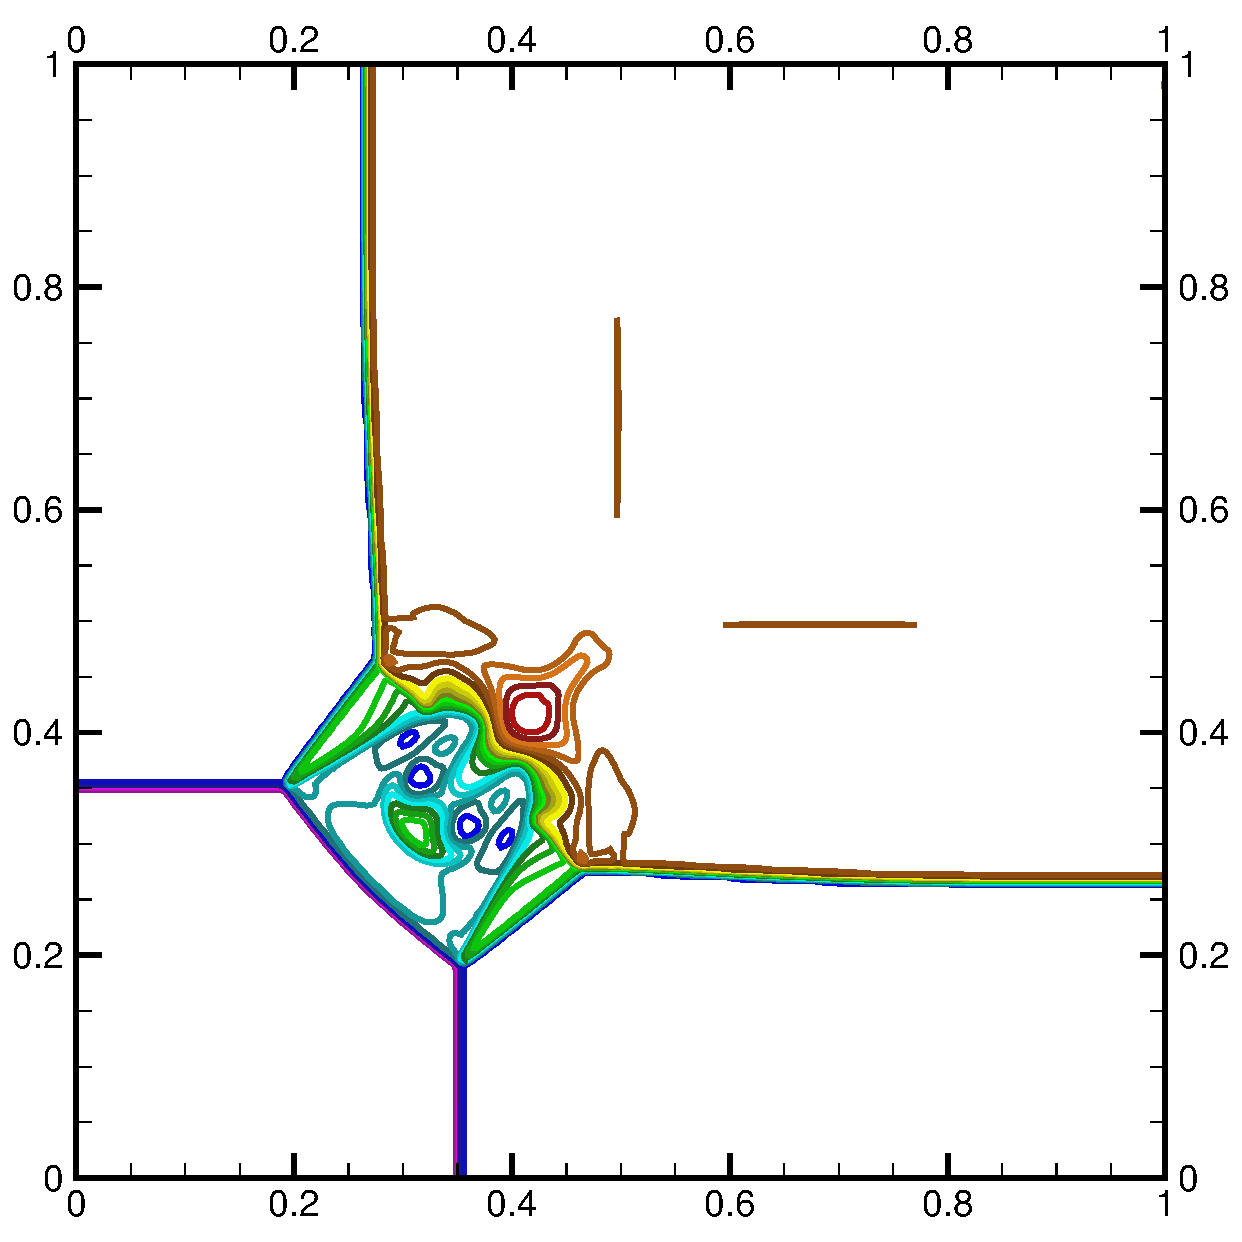
\includegraphics[height=0.4\textheight]{fig/2D/RP1_S2O4-WHC8_CFL0.500000.pdf}
      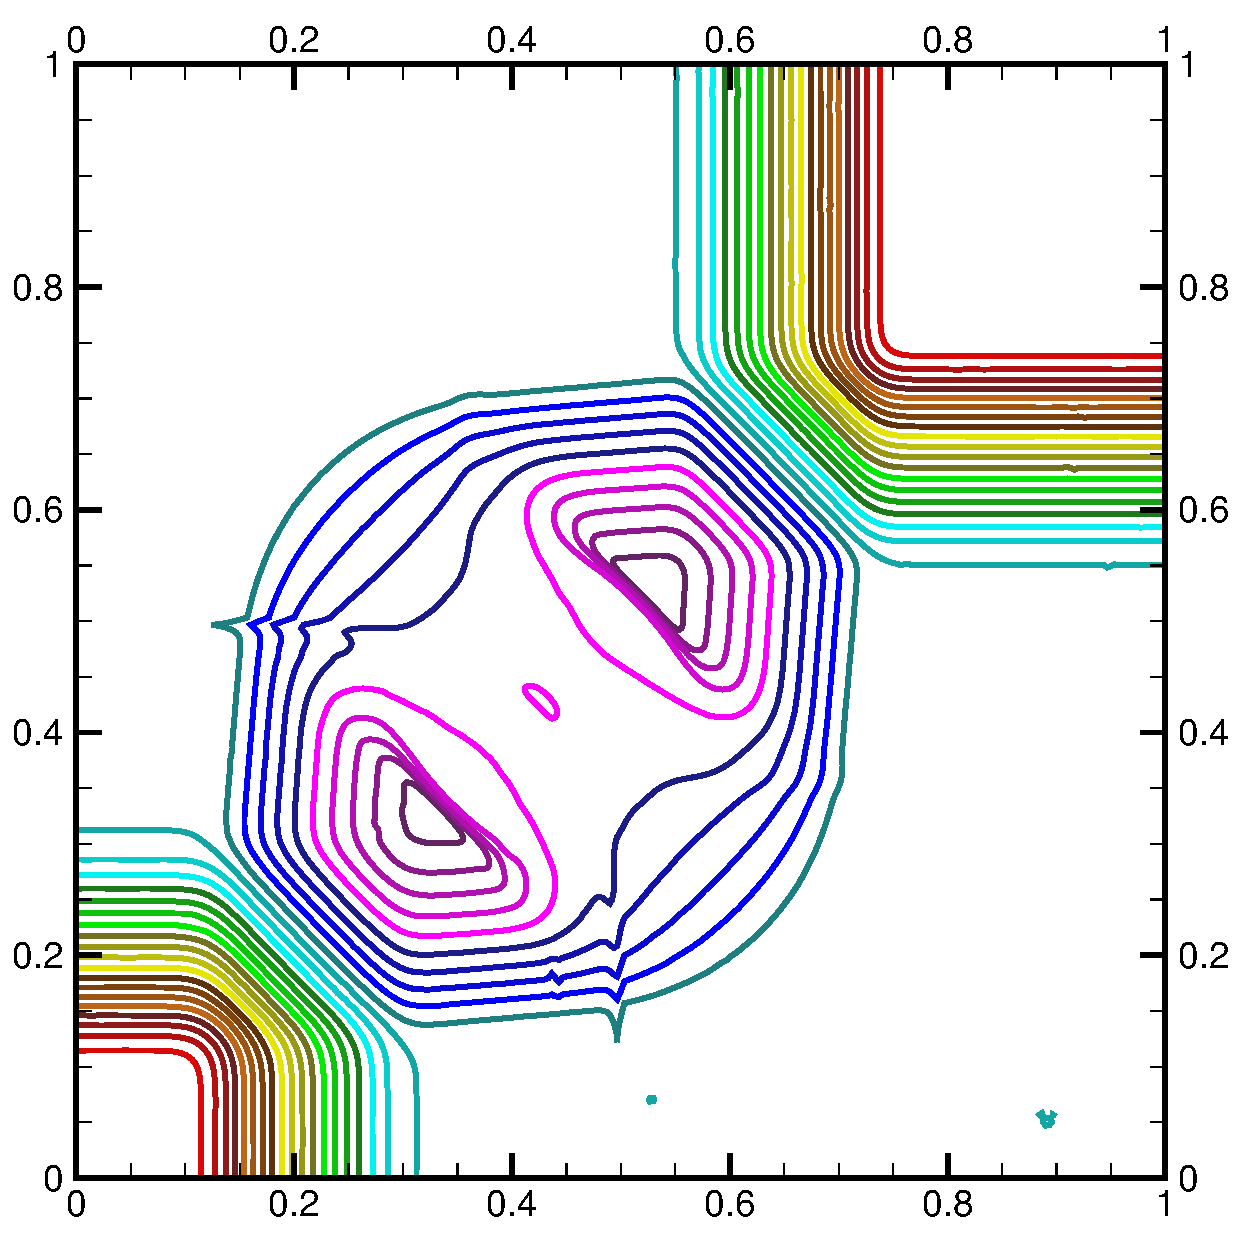
\includegraphics[height=0.4\textheight]{fig/2D/RP14_S2O4-WHC8_CFL0.500000.pdf}
      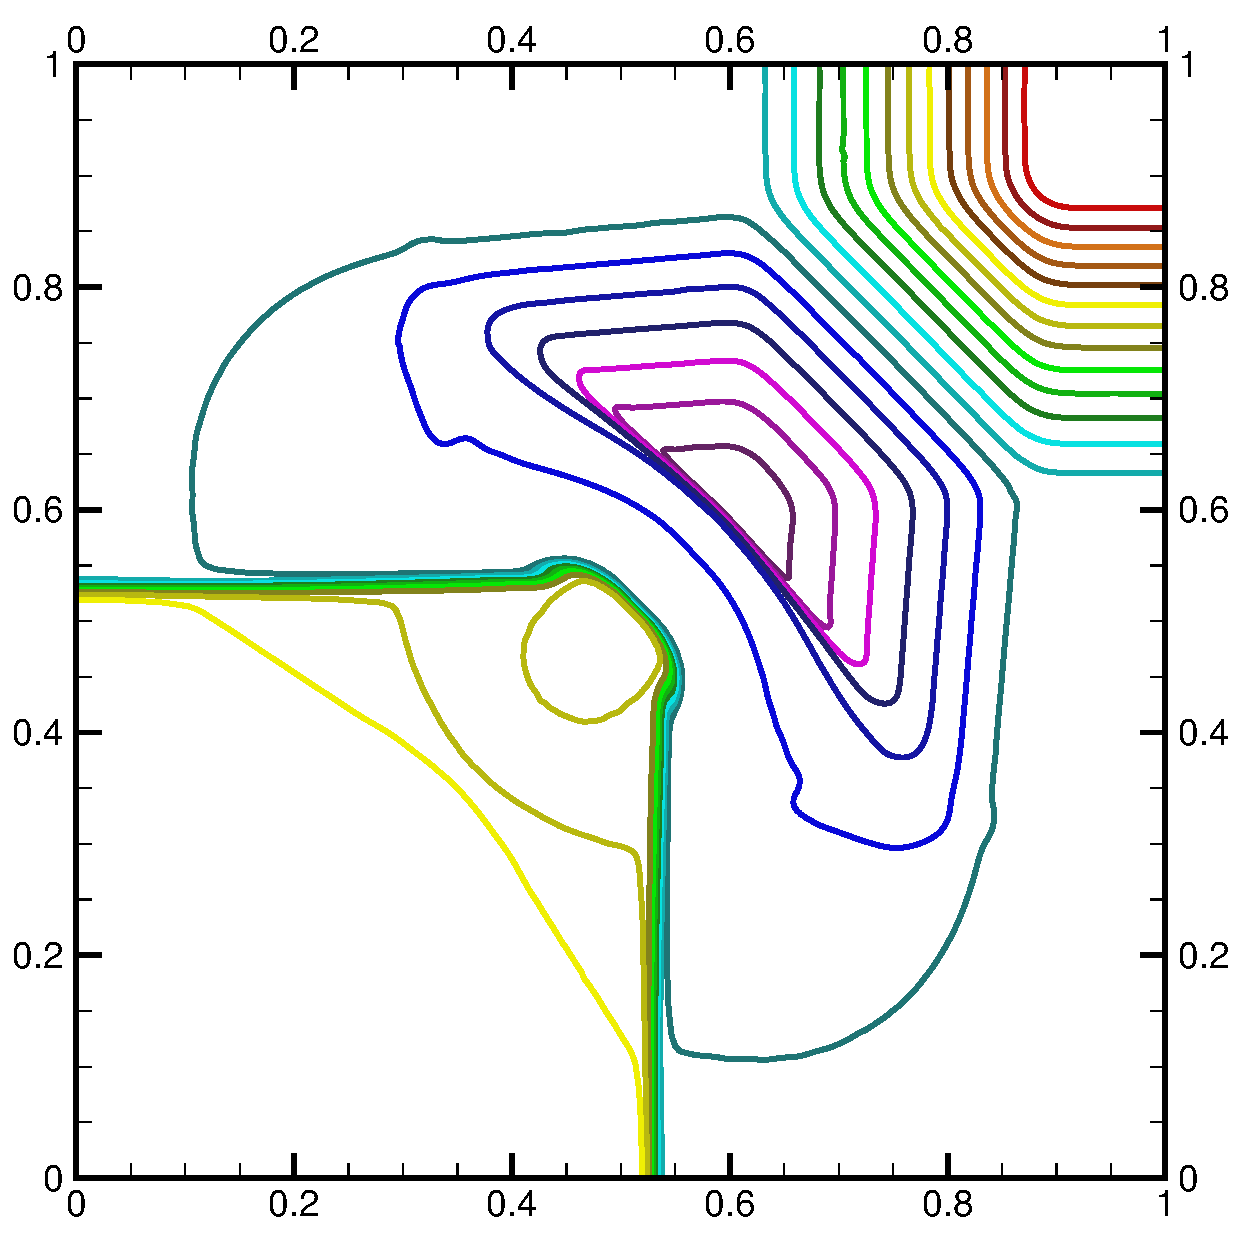
\includegraphics[height=0.4\textheight]{fig/2D/RP15_S2O4-WHC8_CFL0.500000.pdf}
    \end{multicols}
    
    \begin{multicols}{4}
      \begin{minipage}{0.25\textwidth}
        \vspace{0.1\textheight}
        \centerline{HHC-4格式}
      \end{minipage}
      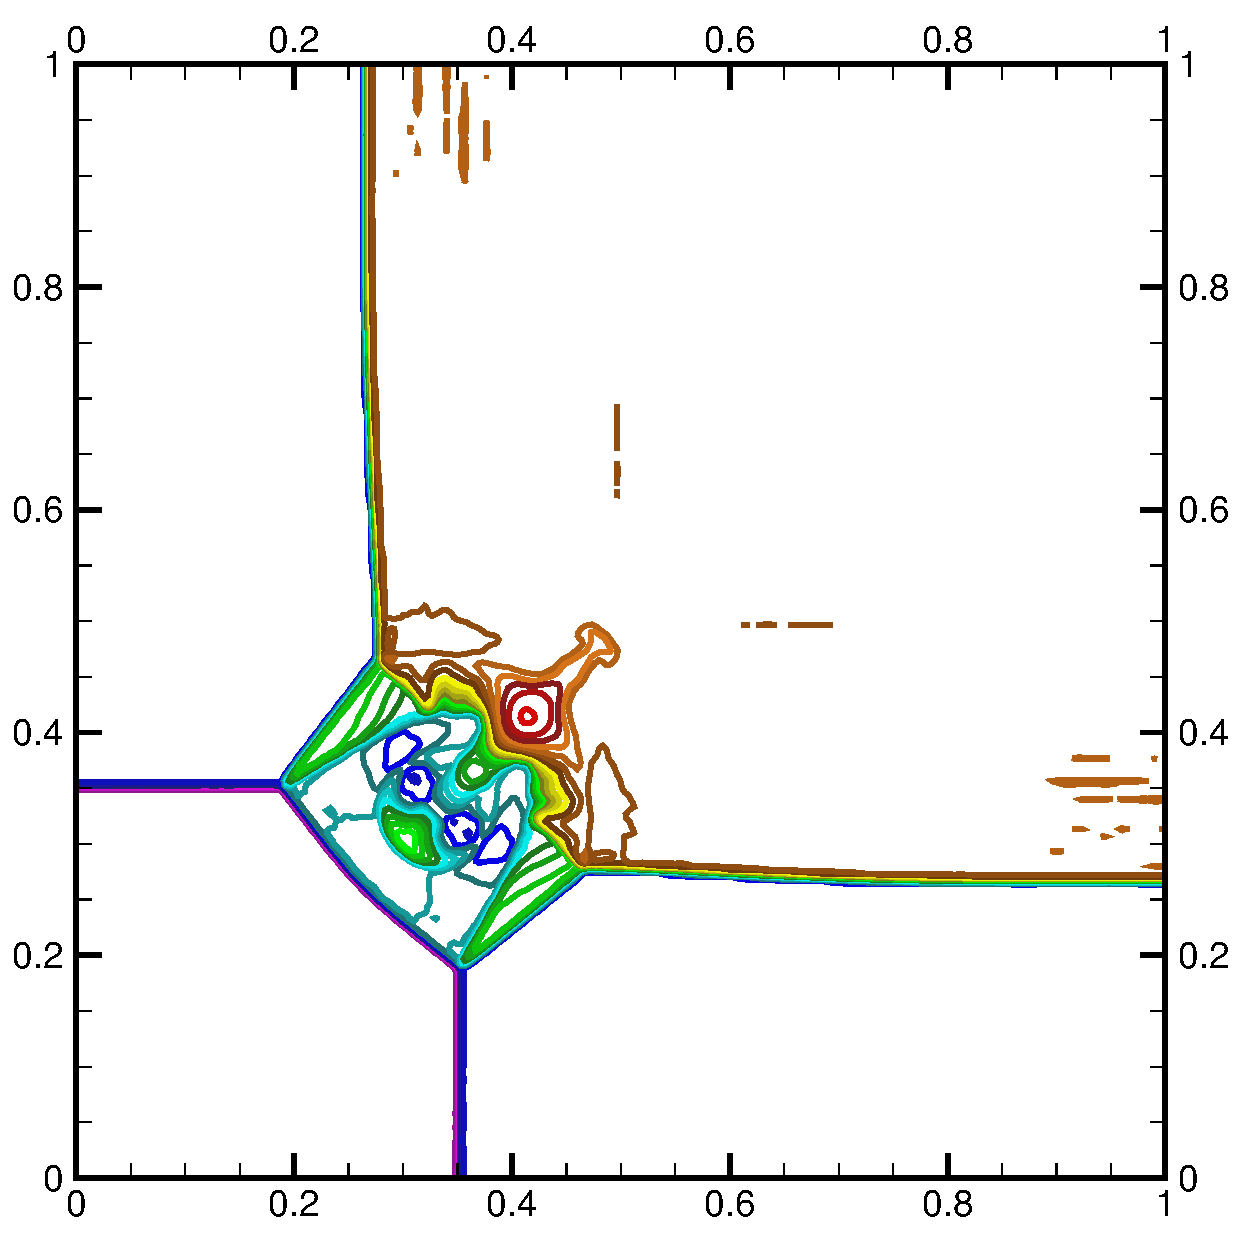
\includegraphics[height=0.4\textheight]{fig/2D/RP1_S2O4-HHC8theta200000_CFL0.500000.pdf}
      \includegraphics[height=0.4\textheight]{fig/2D/RP14_S2O4-HHC8theta200000_CFL0.500000.pdf}
      \includegraphics[height=0.4\textheight]{fig/2D/RP15_S2O4-HHC8theta200000_CFL0.500000.pdf}
    \end{multicols}
  \end{figure}
  
\end{frame}

\begin{frame}{数值格式的时间效率}
  
  \centering
  \includegraphics[height=0.75\textheight]{fig/Time/Time-2D.pdf}
  
\end{frame}

\section{总结}

\begin{frame}{总结}
  
  \begin{itemize}[<+->]
    \item \hl{我们提出了改进的两步四阶时间推进框架。}
          我们分析了原始的时间推进框架掉阶的原因,
          并在此基础上提出了改进的两步四阶时间推进框架。
          在改进的框架中导数重构采用更加紧致的Hermite重构时,
          获得的数值格式可以在光滑区域保持四阶精度。
    \item \hl{我们设计了一维基于紧致Hermite重构的基本无振荡的两步四阶数值格式。}
          然后给了许多算例,
          验证了我们的一维数值格式具有高精度、稳定、紧致、高效以及基本无振荡的优良特性。
    \item \hl{我们设计了二维基于紧致Hermite重构的基本无振荡的两步四阶数值格式。}
          然后给了许多算例,
          验证了我们的二维数值格式具有高精度、稳定、紧致、高效以及基本无振荡的优良特性。
  \end{itemize}
  
\end{frame}

\section*{攻读博士学位期间完成的学术论文}

\begin{frame}{发表的学术论文}
  
  \newcounter{pubctr}
  \begin{list}{[\arabic{pubctr}]}
    {
      \usecounter{pubctr}
      \setlength{\leftmargin}{2.5em}
      \setlength{\labelsep}{1em}
      \setlength{\itemsep}{3ex}
    }
    
    \item \hl{Ang Li}, Jiequan Li. Lax-wendroff solvers-based Hermite reconstruction for hyperbolic problems[J]. Applied Mathematics and Computation, 2023, 447: 127915.
          
    \item \hl{Ang Li}, Jiequan Li, Juan Cheng and Chi-Wang Shu, High order compact Hermite reconstructions and their application in the improved two-stage fourth order time-stepping framework for hyperbolic problems: two-dimensional case[J]. Communications in Computational Physics, Accepted.
  \end{list}
  
\end{frame}

\AtEndDocument{
  \setbeamertemplate{footline}{}
  \ThankFrame % 感谢
  \RefFrame % 参考文献
}

\end{document}